\documentclass [11pt, twoside] {uwthesis}[2012/06/19]

\usepackage{amsmath, graphicx, natbib, listings, lscape, longtable,hyperref}
\def\bibpreamble{\protect\addcontentsline{toc}{chapter}{Bibliography}}

\setcounter{tocdepth}{1}  % Print the chapter and sections to the toc

\usepackage{alltt}  %
\newenvironment{demo}
  {\begin{alltt}\leftskip3em
     \def\\{\ttfamily\char`\\}%
     \def\{{\ttfamily\char`\{}%
     \def\}{\ttfamily\char`\}}}
  {\end{alltt}}

% metafont font.  If logo not available, use the second form
%
% \font\mffont=logosl10 scaled\magstep1
\let\mffont=\sf
% --- end-of-sample-stuff ---

\begin{document}

% ==========   Preliminary pages
%
% ( revised 2012 for electronic submission )
%

\prelimpages

%
% ----- copyright and title pages
%

\Title{Source, propagation, and effects of lightning in the Earth-ionosphere system}
\Author{Michael L. Hutchins}
\Year{2014}
\Program{UW Department of Earth and Space Sciences}

\Chair{Robert H. Holzworth}{Professor}{Department of Earth and Space Sciences}
\Signature{Michael P. McCarthy}
\Signature{Abram R. Jacobson}
\Signature{John M. Wallace}
\Signature{John D. Sahr}

\copyrightpage

\titlepage

%
% ----- abstract
%

\setcounter{page}{-1}
\abstract{

In this dissertation the capabilities of the World Wide Lightning Location Network (WWLLN) are expanded to enable research of the source, propagation, and effects of lightning in the Earth-ionosphere system.
The main expansion of the network is the measurement of the very low frequency radiated energy from lightning; the radiated stroke energy is directly proportional to the canonical peak current measurements of other ground based networks.
Stroke energy is used to develop a model of the network relative detection efficiency; this internal model rates the coverage capabilities of the network compared to the networks best coverage.
The third dataset developed and discussed is the clustering of the lightning locations into both flashes and the active lightning regions of thunderstorms.
These three capabilities of the network allow tracing the effects of lightning and thunderstorms from their source to the global electric circuit and to the magnetosphere.

The source of lightning is investigated in two regimes: within thunderstorms and between thunderstorms.
Within thunderstorms the time between flashes is found to be proportional to the resulting flash energy for differing thunderstorms, regions, and seasons.
Between thunderstorms the lightning energy is shown to differ between land and ocean, with oceanic thunderstorms producing stronger and fewer strokes.
The propagation of the radiated energy is measured using the lightning as a probe of attenuation over along the different propagation paths.
Attenuation is seen to have an asymmetry with magnetic azimuth: eastward moving waves are attenuated less than westward moving waves.
The attenuation asymmetry is complimentary to the observed asymmetry in whistler and radio energy emitted through the ionosphere into the magnetosphere.
Thunderstorm clusters are used to estimate the total upward current contribution of thunderstorms to the global electric circuit.
It is shown that WWLLN can provide one of the first continuous global measurements of this current to the global electric circuit.

}

%
% ----- contents & etc.
%

\tableofcontents
\listoffigures

\listoftables  % I have no tables

%
% ----- glossary
%

%\chapter*{Glossary}      % starred form omits the `chapter x'
%\addcontentsline{toc}{chapter}{Glossary}
%\thispagestyle{plain}
%
%\begin{glossary}
%\item[WWLLN] a network.

%\end{glossary}

%
% ----- acknowledgments
%

\acknowledgments{
I would like to thank everyone in the University of Washington Earth and Space Sciences department: colleagues, classmates, mentors, advisors, and friends.
I want to thank my advisor Robert Holzworth for providing the environment to succeed and develop from the start to the end of my degree.
Michael McCarthy, Abram Jacobson, and John Wallace have helped throughout with discussions of ideas, methods, and research.

I would like to thank Ariah Kidder for providing guidance, mentorship, and much needed distractions.
From across campus I want to thank James Pfeiffer for the math, programming, and fun.
Finally I want to thank my wife Leah for the constant support and encouragement for finishing in a timely manner.
}

%
% ----- dedication
%

\dedication{\begin{center}To Leah\end{center}}

%
% end of the preliminary pages

%
% ==========      Text pages
%

\textpages

% ========== Chapter Introduction

\chapter{Introduction}
\label{thesis:chapter:introduction}

This thesis explores the capabilities and information of ground based lightning detection networks.
What are the limits of what lightning networks can measure?
How can these networks be expanded and what are the effects of these expansions?
Can choosing the right algorithm reveal larger structures from individual lightning strokes?

From these questions lightning, thunderstorms, and the Earth-Ionosphere system can be explored.
The electrical energy in thunderstorms is investigated in how it discharges, where the energy goes, and how does it contribute to the system as a whole.

%% Introductory text / summary / expanded abstract

\section{Background}

\subsection{Lightning and Thunderstorms}

Lightning is the discharge process of disparate charge regions in, typically, a thunderstorm.
When charge is separated in a thunderstorm, a hurricane, a volcanic ash plume, or on other planets it eventually discharges in order to neutralize the charge imbalance.
Typically this occurs through lightning flashes.

In a thunderstorm deep convection develops, lifting moist air from below the thunderstorm up through the cloud where the moisture begins to precipitate.
Figure~\ref{intro:fig:thunderstorm} shows the basic components of an active thunderstorm.
As the water droplets begin to freeze as they pass through the freezing level of the thunderstorm, at this freezing level they collide with downwelling ice particles.
At these collisions charge exchange causes the downwelling ice to gain a negative charge and the upwelling water to become positively charged.
This leads to the gross charge structure shown in Figure~\ref{intro:fig:thunderstorm}, with positive charge at the top of the thunderstorm and negative charge at the bottom.

\begin{figure}[ht!]
	\centering
	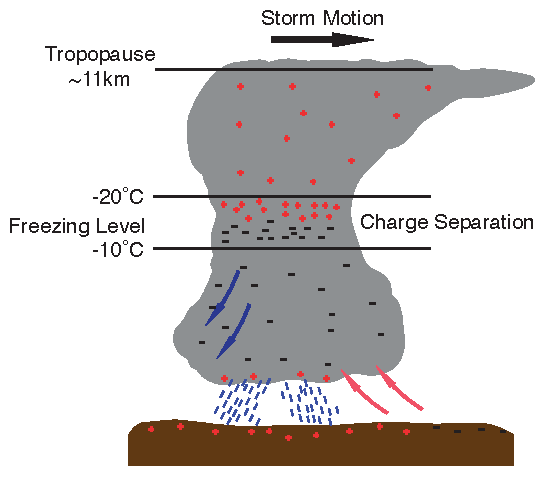
\includegraphics[scale=1]{Introduction/Figures/Thunderstorm_Structure.pdf}\\
	\caption{Overall thunderstorm structure showing the general charge distribution.}
	\label{intro:fig:thunderstorm}
\end{figure}

When enough charge is separated the stepped-leader process begins.
While an appreciable voltage builds up between the charge centers (the thunderstorm and ground for example) on the order of $MV$ it is still far less than the breakdown voltage of air.
However the air is broken down in \~100~$m$ steps that leaves an ionized plasma channel; the breakdown process is semi-fractal with steps occurring until an oppositely charge region is connected.
The process for the step-leader breakdown is shown in Figure~\ref{intro:fig:evolution}.

For the first 20~$ms$ the step leader creates the ionized channel to ground (or another charge region).
Once the channel is established the return stroke moves charge from the ground to the cloud over the course of 70~$\micro s$.
After the return stroke the top of the ionized channel can connect to other charge regions through a subsequent step-leader process producing multiple return strokes along the same channel.
The total step-leader through multiple return strokes is considered a single lightning flash.

\begin{figure}[ht!]
	\centering
	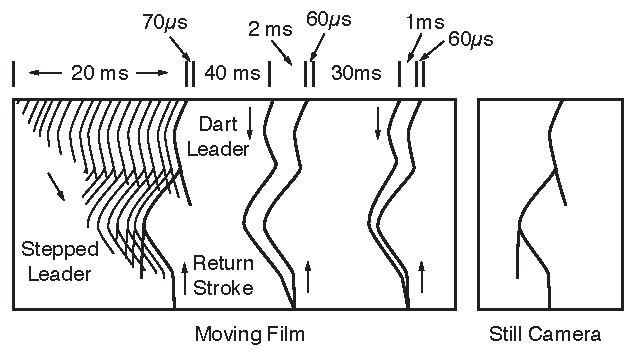
\includegraphics[scale=1]{Introduction/Figures/Lightning_Evolution.pdf}\\
	\caption{The step-leader and discharge process of cloud to ground lightning with typical times of each event.}
	\label{intro:fig:evolution}
\end{figure}

%% Lightning types
%% Their rough ratios
%% Lightning like discharges (TGF, NBE, TLE)

\begin{figure}[ht!]
	\centering
	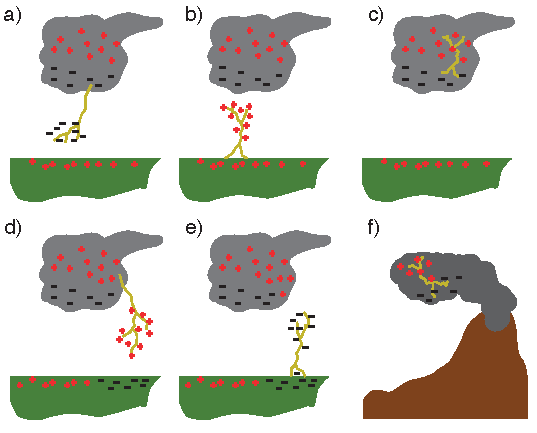
\includegraphics[scale=1]{Introduction/Figures/Lightning_Types.pdf}\\
	\caption{}
	\label{intro:fig:types}
\end{figure}




\subsection{The Ionosphere}

%% What is the ionosphere
%% What forms the ionosphere

%% General trends in behavior - day/night
%% Important properties: conductive, plasma, collisions

\begin{figure}[ht!]
	\centering
	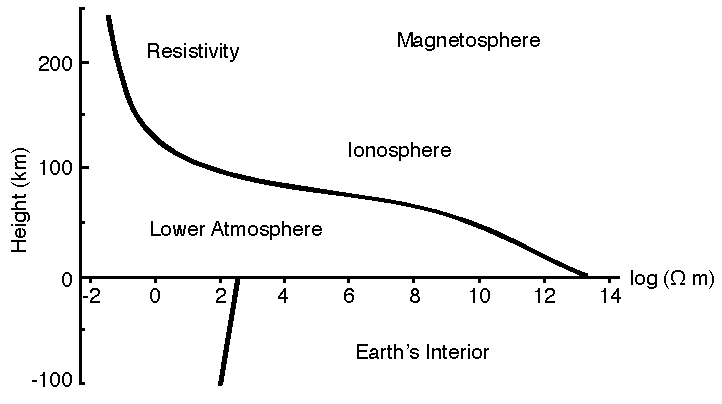
\includegraphics[scale=1]{Introduction/Figures/Atmospheric_Conductivity.pdf}\\
	\caption{}
	\label{intro:fig:ionosphere}
\end{figure}

%% VLF wave propagation in the ionosphere
%% Frequencies that transfer well (ELF, VLF)
%% Distance of VHF

%% Losses due to heating and plasma / whistler mode waves
%% Losses to the ground (water < ground < ice)
%% Distances that can be measured

\begin{figure}[ht!]
	\centering
	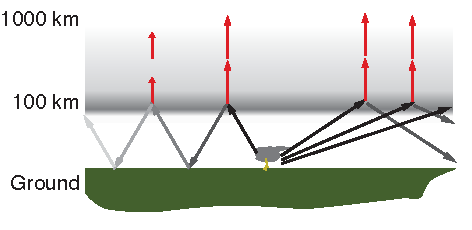
\includegraphics[scale=1]{Introduction/Figures/EIWG.pdf}\\
	\caption{}
	\label{intro:fig:eiwg}
\end{figure}

\subsection{Global Electric Circuit}

The global electric circuit is the current system formed by the ionosphere and ground acting as leaky spherical capacitors, as shown in Figure~\ref{intro:fig:gec}a with an equivalent circuit in Figure~\ref{intro:fig:gec}b.
Thunderstorms are the primary drivers of the circuit with the charged ionosphere discharging through fair weather.
Diurnal variation in global thunderstorm activity was original observed by \citet{Wilson1921} and \citet{Whipple1929} through a combination of thunderstorm day and electric field measurements.
Strong correlations between thunderstorm activity and fair weather return current led to the current model of the global electric circuit.
The global electric circuit changes activity changes on short time scales that are not resolved with past models or with long term averaged observations.
The global electric circuit is an important component to the solar-terrestrial system creating a link between solar activity, the ionosphere, aerosols, cloud microphysics, thunderstorms, weather, and climate \citep{Tinsley2007, Holzworth1986}.

\begin{figure}[ht!]
	\centering
	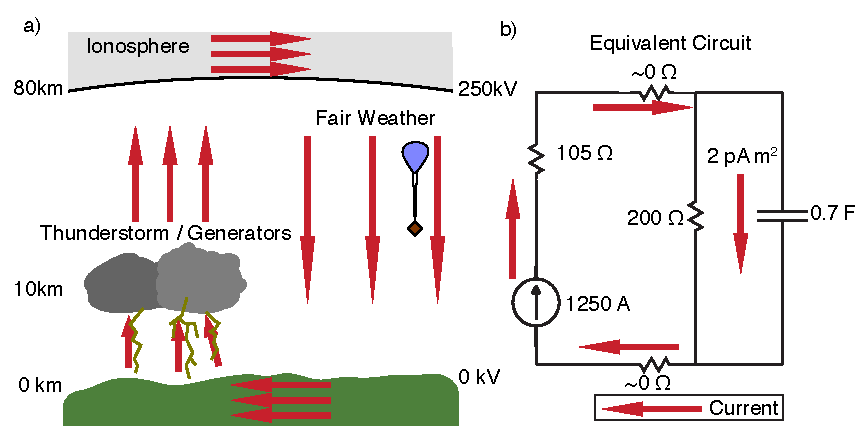
\includegraphics[scale=1]{Introduction/Figures/Global_Circuit.pdf}\\
	\caption{}
	\label{intro:fig:gec}
\end{figure}

\section{Lightning Detection Systems}

There is a growing importance, both scientifically and operationally, of ground based lightning detection networks.
Lightning detection networks are being used in a larger gamut of research areas including: terrestrial gamma ray flashes \citep{Dwyer2012, Gjesteland2011, Connaughton2010}, lightning climatology \citep{Virts2013, Virts2011a, Burgesser2012}, ionospheric disturbances and probing \citep{Jacobson2010, Singh2011}, transient luminous events \citep{Soula2011}, global electric circuit  \citep{Holzworth2005}, and whistler observation \citep{Collier2010, Collier2011a, Burkholder2013}.
This is in conjunction with the extended usage of lightning networks operationally in weather prediction and tracking \citep{Fierro2012, Pan2010, Thomas2010d}, volcano monitoring \citep{Doughton2010}, and hazard estimation \citep{Altaratz2010}.
With growing usage it is necessary to understand the capabilities and efficiencies of the various available lightning networks.

Ground based total lightning networks distinguish themselves from other ground based networks and satellites by detecting and identifying in-cloud (IC) discharges as well as cloud to ground (CG) strokes.
Lightning type is critical in understanding thunderstorm dynamics \citep{Williams1989}, with real time monitoring of sudden increases of IC activity able to predict severe weather events \citep{Rudlosky2013, Darden2010, Metzger2013, Schultz2009, Schultz2011}.
The higher frequencies of total lightning networks are also useful for researching narrow bipolar events \citep{Suszcynsky2003} and large scale lightning behavior \citep{Hutchins2013}.
Lightning mapping arrays are able to locally detect, locate, and distinguish IC activity, however total lightning networks have the advantage of much larger spatial coverage.

\subsection{World Wide Lightning Location Network}

%% Add in global stroke distribution figure

%% Update with more recent papers
The World Wide Lightning Location Network (WWLLN, see http://wwlln.net) determines the location for nearly all lightning producing storms around the globe in real time (c.f. \citet{Jacobson2006c}).
WWLLN has been generating global lightning locations starting in 2004 \citep{Rodger2006, Rodger2009}.
Since then the network has grown from 18 stations to over 70 as of September 2013.
Knowledge of individual stroke locations, with high temporal accuracy, and within a fraction of a wavelength is beneficial for both scientific and technical uses.
WWLLN lightning location data have recently been used for advances in space science \citep{Lay2007, Kumar2009, Collier2009, Holzworth2011, Jacobson2011}, meteorology \citep{Price2009,Thomas2010d}, detailed lightning physics \citep{Connaughton2010}, and volcanic eruption monitoring \citep{Doughton2010}.

The network uses a time of group arrival (TOGA) technique, originally developed by \citet{Dowden2002d}, to locate strokes by analyzing the sferic waveforms at each station using the Stroke\_B algorithm as discussed by \citet{Rodger2006,Rodger2009}.
WWLLN locates strokes by analyzing the TOGA of the sferic wave packet in the 6 -- 18~kHz band \citep{Dowden2000}.
The TOGA of the VLF wave packet, is used rather than ``trigger time'' to produce more uniform arrival times across the network.
A recent upgrade to the network allows for the measurement of the radiated VLF energy of located strokes within the 8 -- 18~kHz VLF band.
The stroke energy is calculated from the time-integrated root mean square (RMS) electric field of the VLF sferic at each WWLLN station, using the Long Wave Propagation Capability code (LWPC) \citep{Ferguson1998} to estimate the sferic attenuation and calculate the source radiated energy \citep{Hutchins2012}.

As stations are added the accuracy and detection efficiency of the network improves.
As of 2010 the network locates most strokes to within 10 kilometers and $<$10~$\mu$s with an estimated detection efficiency of about 11\% for all strokes and $>$30\% for more powerful strokes \citep{Abarca2010,Rodger2009}.
The network improves in accuracy and detection efficiency with increased stations; for example an increase in the number of WWLLN stations from 11 in 2003 to 30 in 2007 led to a $\sim$165\% increase in the number of lightning strokes located \citep{Rodger2009}.
However the WWLLN network does not observe lightning with the same detection efficiency everywhere.
This is due to variable WWLLN station coverage and the strong affect on VLF radio propagation from orography and ionospheric conditions along the great circle path of a wave.

\subsection{Earth Networks Total Lightning Network}

%% Add ENTLN stroke density figure

The Earth Networks Total Lightning Network (ENTLN) is a ground based network that began in 2009 as the Weatherbug Total Lightning Network (WTLN).
It has two operational regimes: short range using broadband sferic waveforms (5~kHz -- 12~MHz) and long range with only VLF waveforms (1~Hz -- 256~kHz) \citep{Heckman2010}.
Correlations of the stroke waveform and amplitude from multiple stations determines the time, location, altitude, peak current, polarity, and type of the located stroke \citep{Liu2011a}.
The network utilizes a time of arrival method to determine the location of each stroke, where a minimum of 8 stations is required to produce a valid solution.
To compress the broadband waveforms each station removes the necessary amount of low-amplitude signal to reach the requisite packet size.
In the continental United States (CONUS) the network has approximately 530 operational stations in September 2013.
A comparison to the Oklahoma Lightning Mapping Array (OKLMA) in 2010 demonstrated the ability to discriminate between CG and IC strokes \citep{Beasley2010}.

\subsection{TRMM/LIS}

%% Add LIS global flash count figure.

The Lightning Imaging Sensor (LIS, 1997-present) is a satellite-based lightning detector flown onboard the Tropical Rainfall Measurement Mission (TRMM) satellite orbiting at a 35$^\circ$ inclination and 402~km altitude \citep{Christian1999}.
In low earth orbit it observes the total lightning activity from individual thunderstorms for 90 sec in each $0.5^\circ \times 0.5^\circ$ viewtime granule.
LIS is useful as it is a lightning detection system with no overlapping detections methods with ground based networks, and the sensor performance has not changed over time.
The LIS data are available at several processed levels, throughout this work the flash level data is used.

\section{Long Wave Propagation Capability Code}

The Long Wave Propagation Capability code (LWPC) is used to model the VLF attenuation between WWLLN located lightning and the network stations.
The LWPC code was developed by the Space and Naval Warfare Systems Center by \citet{Ferguson1998} and has most recently been validated by \citet{McRae2000d, Thomson2011}.
In this research we made use of an adapted LWPC version 2.1.

LWPC can be used to model the attenuation along a mixed day/night ionospheric path, however due to computational limitations a lookup table is used instead.
The lookup tables model the received electric field at a given station for a 100~kW transmitter in each grid cell.
A $1^{\circ}$ by $1^{\circ}$ grid is used for either an all day ($\beta=0.3$ km$^{-1}$ and $h'=74$ km) or an all night ($\beta(f)=0.3-0.8$ km$^{-1}$ and $h'=87$ km) ionospheric model, where $\beta$ and $h'$ are the slope of the conductivity ($\beta$ is frequency dependent at night) and the reference height in the ionospheric model.
The ionospheric models are the default models of LWPC code and fully described in \citet{Ferguson1998}. 

For each grid cell the electric field is averaged over the 8 -- 18 kHz band, which captures the frequencies of the peak radiated power from lightning \citep{Volland1995}.
An example of the day ionosphere lookup table for the Dunedin station is shown in Figure~\ref{intro:fig:lookup} (reproduced from Chapter~\ref{thesis:chapter:efficiency}).
The discontinuity of electric field over Greenland and in the South Atlantic is caused by the high attenuation rate of VLF propagating over ice.
Using the lookup tables assumes that the attenuation rates do not vary greatly within a given grid cell and that the frequency spectra of a sferic is relatively flat within the band considered.

\begin{figure}[ht!]
	\centering
	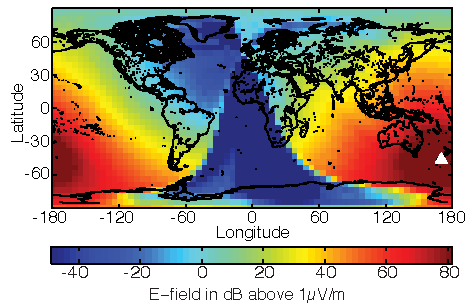
\includegraphics[scale=1]{energy/Figures/PPS_Lookup.pdf}\\
	\caption{LWPC generated lookup table for Dunedin station (white triangle) using an all day ionospheric model ($	\beta=0.3$ km$^{-1}$ and $h'=74$ km) averaged over 8-18 kHz. Each $1^{\circ}$ by $1^{\circ}$ bin shows the electric field seen at Dunedin if a 100kW transmitter is centered on that bin.}
	\label{intro:fig:lookup}
\end{figure}

\section{Outline}

In Chapter~\ref{thesis:chapter:energy} the process for calculating the far-field radiated VLF energy of lightning with WWLLN is described.
The work is adapted from the \citet{Hutchins2012} paper.
Chapter~\ref{thesis:chapter:efficiency} discusses the relative detection efficiency model of WWLLN.
The work is from the \citet{Hutchins2012a} paper.
The network improvements of Chapters~\ref{thesis:chapter:energy} and~\ref{thesis:chapter:efficiency} enables the work in Chapters~\ref{thesis:chapter:landsea} and~\ref{thesis:chapter:landsea}.

Chapter~\ref{thesis:chapter:landsea} examines the contrast between oceanic and continental lightning using the WWLLN stroke energy measurements with a linear regression method developed in the chapter.
This research is adapted from the \citet{Hutchins2013}.
Chapter~\ref{thesis:chapter:prop} combines the WWLLN energy measurements with the LWPC code to estimate the VLF attenuation rates over ocean in the day and night ionospheric regimes.
This research is adapted from the \citet{Hutchins2013a}.
Chapter~\ref{thesis:chapter:gec} applies a clustering algorithm to the WWLLN stroke locations, producing thunderstorm clusters, to create a prediction of the global electric circuit activity.
%% Update status as needed
This research is currently submitted and under review.

Appendix~\ref{thesis:appendix:code} describes the different types of WWLLN data files available, their location, and the common code used in this thesis (code for individual chapters can be made available upon request).
Notably the code for the energy calculations (Chapter~\ref{thesis:chapter:energy}), relative detection efficiency model (Chapter~\ref{thesis:chapter:efficiency}), and thunderstorm clustering (Chapter~\ref{thesis:chapter:gec}) are available online.
Appendix~\ref{thesis:appendix:energy} describes the WWLLN stroke energy code and operations, enabling both reproduction of the results and steps to setup new energy processing computers.

Appendix~\ref{thesis:appendix:su} and~\ref{thesis:appendix:gumstix} describe the development, construction, and operation of the WWLLN Service Unit v4 computers.
Schematics, EAGLE files, parts list, software, and operations are all described with the code available as described in Appendix~\ref{thesis:appendix:code}.


% ========== Chapter Stroke Energy

\chapter{Stroke Energy}
\label{thesis:chapter:energy}

\section{Overview}

The World Wide Lightning Location Network (WWLLN) is a long range network capable of locating lightning strokes in space and time.
While able to locate lightning to within a few kilometers and ten microseconds, the network currently does not measure any characteristics of the strokes themselves.
The capabilities of the network are expanded to allow for measurements of the far-field energy from the root mean square electric field of the detected strokes in the 6 -- 18~kHz band.
This is accomplished by calibrating the network from a single well calibrated station using a bootstrapping method.
With this technique the global median stroke energy seen by the network is 1.3 x $10^3$~J with an average uncertainty of 17\%.
The results are validated by comparing to return stroke peak current as measured by the New Zealand Lightning Detection Network and to previous ground wave power measurements in the literature.
The global median stroke energy is found to be 2\% of previous measurements of radiated electromagnetic energy.
Accounting for the different observational distances, we find our far-field observations of the waveguide mode are consistent with the previous literature
This study demonstrates that the WWLLN determined energies can be used to estimate the return stroke peak currents of individual lightning strokes occurring throughout the globe.

\begin{figure}[ht!]
\centering
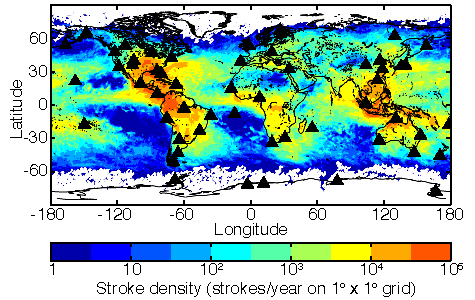
\includegraphics[scale=1.5]{energy/Figures/PPS_WWLLN_2010.pdf}\\
\caption{WWLLN 2010 global stroke density on $1^\circ$ x $1^\circ$ grid, station locations shown with black triangles. Data processed with the Stroke\_B algorithm.}
\label{energy:fig:wwlln_dist}
\end{figure}

As only the spectral variations through the sferic wave packet are needed for determining the TOGA, the absolute electric field amplitude is unnecessary to accurately locate lightning. Due to this, the network does not currently report other characteristics of strokes such as peak current.
However, each WWLLN station does record the root mean square (RMS) electric field value of the sferic waveform used in the TOGA calculation, but these values need to be calibrated, as discussed below.

The station operated by the University of Otago near New Zealand's Antarctic station, Scott Base, was calibrated by a field team in December 2009.
The field team injected a series of calibration signals, ramped progressively in frequency, through the crossed magnetic loops of the Scott Base antenna and computed the calibration from the equivalent electric field.
This calibration of a single station allows for the calculation of stroke energy as seen by the network.

A previous study by \citet{Rodger2006} attempted to calibrate the network through observations of narrow-band VLF communication transmitters at each WWLLN station.
These observations were combined with the U.S. Navy Long Wave Propagation Capability (LWPC) code, described by \citet{Ferguson1998}, to predict what the received amplitude should be in order to calibrate each station.
However the study assumed that the frequency response and calibration of the sound cards was the same across the network, assumptions that are false.
In fact, the sound cards, preamplifier, and antenna vary by a factor of 10 in their sensitivity. 
The current study utilizes a broader range of frequencies and calibrates each station such that differing frequency responses are accounted for in the calibration.

Measuring stroke energy is an important step forward as it allows the network to make real time measurements of the strength of lightning worldwide.
Being able to measure characteristics of the strokes will allow for insights into thunderstorm evolution, large scale storm phenomena, and global effects of lightning.
For example, stroke energy values could help current research on terrestrial gamma ray flashes by \citet{Briggs2011} constraining efficiencies and source mechanisms, and tropical hurricanes by \citet{Thomas2010d} could utilize the energy in analyzing eyewall replacement.

As we will show in this Chapter, the network measures a median global VLF energy power in the far-field waveguide mode of 1.3 x $10^3$~J with an average uncertainty of 17\%.
Previous measurements have shown the energy radiated by strokes is often near $7.0^{4}$~J \citep{Taylor1963}.
Past measurements were measured much closer to that strokes (100~km) and normalize to closer distances, resulting in a measurement of both the sky- and ground-wave of the sferic.
WWLLN measures the RMS electric field at distances where only the waveguide mode of the sferic remains.
When these factors are accounted for the median energy from WWLLN located strokes is comparable to the previously reported value of $7.0^{4}$~J electromagnetic energy.

\section{Instrumentation and Data Processing}

In order to calculate the stroke energy from WWLLN three steps are necessary: calibrate each station in the network, measure RMS electric field of a stroke at each station, and calculate the stroke energy needed to produce the electric field at each station.

\subsection{Station Electric Field}

Each WWLLN station consists of four main components: the antenna, a preamplifier, a service unit for signal and power management, and the sound card that digitizes the measured fields.
The difficulty in making an energy measurement with the network arises in calibrating for the coupling between a short (2m) station antenna to a signal with an approximately $\sim$10~km wavelength.
When a station digitizes the electric field waveform it stores it in uncalibrated sound card units (SCU).
Additionally, the effective gain and calibration differs at each station due to the preamplifier, antenna construction, soundcard frequency response, and local environmental conditions.
This results in the RMS electric field being reported in station specific sound card units.

The average power spectra from 194 stroke waveforms recorded at the Tallahassee, Florida station are shown in figure~\ref{energy:fig:average_spectra} along with the frequency response of a typical preamplifier.
The strokes used were located at distances of 5000~km to 10000~km from the station and were recorded between 18:00 and 21:00 UTC on May 3 and May 9 2011.
As can be seen in the figure the power peaks between 6 -- 18 kHz with the analog response remaining relatively flat through the entire frequency range.
The spikes in the power spectra are a result of manmade VLF communication transmitters.

\begin{figure}[ht!]
\centering
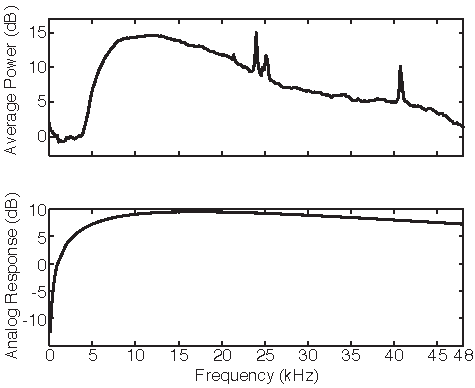
\includegraphics[scale=1]{energy/Figures/PPS_Spectra.pdf}\\
\caption{The top panel shows average power spectra from 194 stroke waveforms recorded at the Tallahassee, FL station between 0 and 48 kHz. The strokes were located between 5~Mm and 10~Mm away from the  station on May 3 2011 and May 9 2011 between 18:00 and 21:00 UTC. The bottom panel shows the frequency response of the preamplifier.}
\label{energy:fig:average_spectra}
\end{figure}

The waveforms used are 1.33~ms long with 0.33~ms pre-trigger and 1~ms post-trigger.
Prior to processing the waveform is put through a 6 -- 18~kHz 16 point finite impulse response (FIR) bandpass filter.
The RMS value of the resultant waveform is stored in uncalibrated sound card units.
After being calibrated to the $\sim$10~km wavelength signal the SCU measurement can be converted into the RMS electric field of the sferic. 

\subsection{LWPC and Energy}

To calculate the stroke energy based on the RMS electric field at a station the LWPC code is used to model the attenuation, as a function of frequency, between a transmitter at the stroke location and the receiving station.
The LWPC code was developed by the Space and Naval Warfare Systems Center by \citet{Ferguson1998} and has most recently been validated by \citet{Thomson2011}.
In this research we made use of LWPC version 2.1.

With a known conversion from a station's SCU value to V m$^{-1}$, $A_{local}$, of the lightning waveform, power is calculated using equation~\ref{energy:eq:power_eq}.
The ratio from LWPC between a 100~kW transmitter and the modeled field (given in dB above 1~$\mu$V m$^{-1}$) is used to account for the sferic attenuation, $\alpha$, along the path for every grid location for every detector.

\begin{equation}
P_{stroke}=\frac{E_{scu}^2}{A_{local}^2} * \frac{100kW}{(10^{\alpha/20}\mu V/m)^2}
\label{energy:eq:power_eq}
\end{equation}

Since energy of the stroke is the time integrated electric field, and the power measurements are from the RMS electric field value, the energy of the stroke can be found from the size of the recording window: $E_{stroke}=P_{stroke} * t_{record}$, with the current recording window set at 1.33 ms.
The power measurement is an intermediary step with all WWLLN stroke strength values measured and recorded in terms of radiated energy.

Due to computing limitations running the LWPC code, we cannot conduct a full run for every stroke-station pair in real time.
Instead a lookup table is used which breaks stroke locations into $1^{\circ}$ by $1^{\circ}$ bins and uses either an all day ($\beta=0.3$ km$^{-1}$ and $h'=74$ km) or an all night ($\beta(f)=0.3-0.8$ km$^{-1}$ and $h'=87$ km) ionospheric model, where $\beta$ and $h'$ are the slope of the conductivity ($\beta$ is frequency dependent at night) and the reference height in the ionospheric model.
The ionospheric models are the default models of LWPC code and fully described in \citet{Ferguson1998}. 
To account for transitions across the terminator a weighted average of the day and night electric field values are used.
The lookup tables give the electric field averaged over the 8 -- 18 kHz band which captures the frequencies of the peak radiated power from lightning (6 -- 7~kHz omitted due to code limitations) \citep{Volland1995}.
An example of the day ionosphere lookup table for the Dunedin station is shown in figure~\ref{energy:fig:lookup}.
The discontinuity of electric field over Greenland and in the South Atlantic is caused by the high attenuation rate of VLF propagating over ice.

\begin{figure}[ht!]
\centering
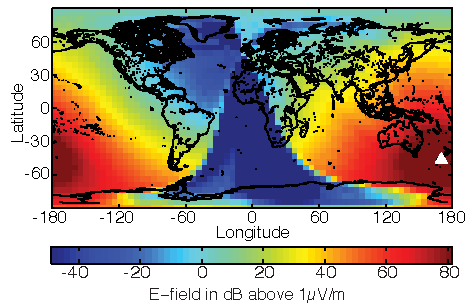
\includegraphics[scale=1]{energy/Figures/PPS_Lookup.pdf}\\
\caption{LWPC generated lookup table for Dunedin station (white triangle) using an all day ionospheric model ($\beta=0.3$ km$^{-1}$ and $h'=74$ km) averaged over 8 -- 18~kHz. Each $1^{\circ}$ by $1^{\circ}$ bin shows the electric field seen at Dunedin if a 100~kW transmitter is centered on that bin.}
\label{energy:fig:lookup}
\end{figure}

\subsection{Calibration and Bootstrapping}

With one calibrated station it is possible to find the calibration of other nearby stations.
The process is shown in figure~\ref{energy:fig:calibrate}.
Using a well calibrated station (on the right) the stroke energy of a given stroke is found using LWPC for the same stroke.
The uncalibrated station also finds the power using LWPC, however instead of a power in watts, it measures the power in sound card power, SCP.
The ratio between the two power values will give the calibration factor, $A_{local}^2$, of the second station.
This is repeated for many strokes with the median of the conversion factor distribution used as the conversion factor between the two stations.

\begin{figure}[ht!]
\centering
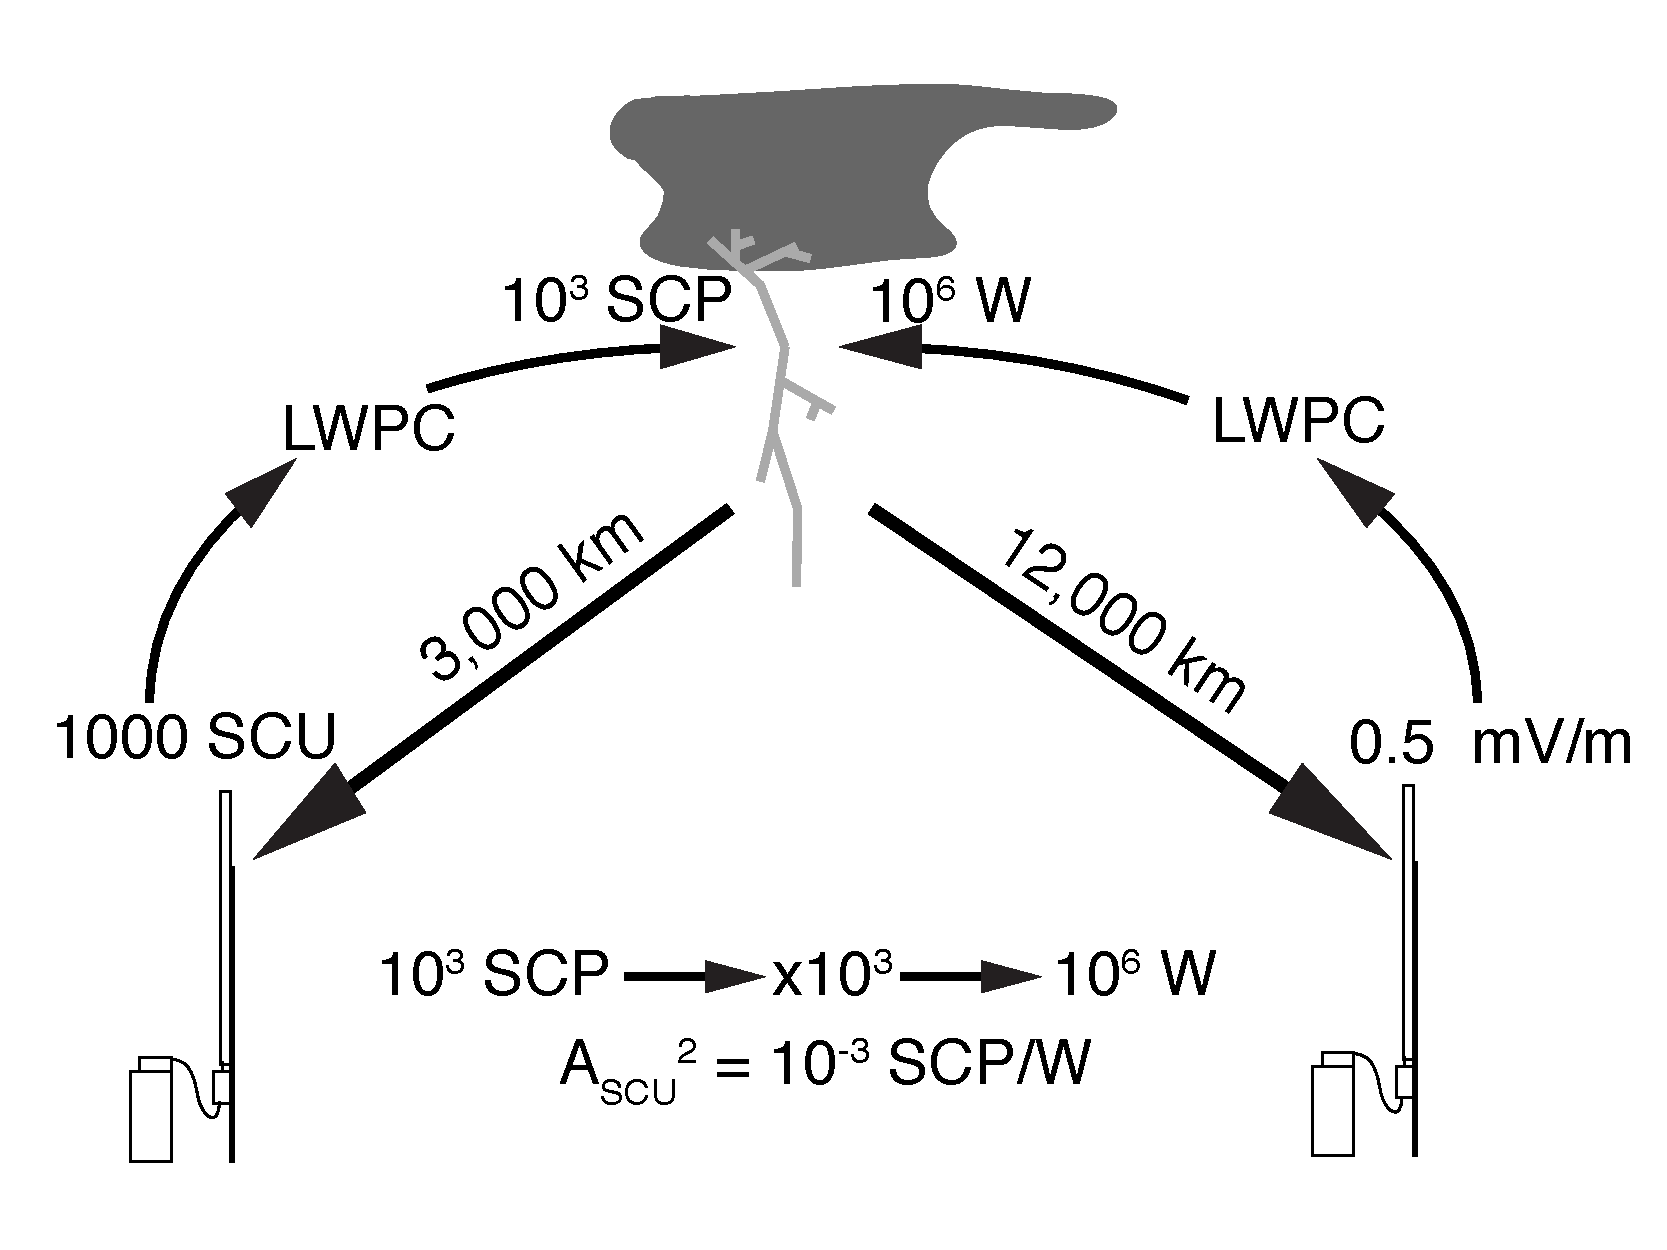
\includegraphics[scale=1]{energy/Figures/PPS_Method.pdf}\\
\caption{Method of calibrating one station to another using LWPC.}
\label{energy:fig:calibrate}
\end{figure}

Only one station in the network is thoroughly calibrated to VLF fields, the station in Scott Base, Antarctica.
Using the method described below the Dunedin station was calibrated off of Scott Base station.
With both stations calibrated, Dunedin was chosen as the first calibrated station in the bootstrapping process, by using thousands of mutually observed sferics.
Dunedin was chosen instead of Scott Base due to strong observed seasonal variations likely due to changes in local ground conductivity that are not accounted for in the propagation model.

To calibrate the entire network off of a single station a bootstrapping method is used.
Station to station calibrations are done using strokes that have all day paths to both stations and are within 1000 -- 8000~km of both stations.
All day paths were chosen as the daytime ionosphere is modeled more accurately by LWPC than the night ionosphere \citep{McRae2000d}.

The first set of calibrations are done between the well calibrated station and those with common strokes that have the desired path characteristics.
Once calibrated these stations are used to calibrate the next set of stations, and these newly calibrated stations are used to find the next set.
This process is repeated until no further stations can be calibrated, figure~\ref{energy:fig:bootstrap} is an example of this process.
Not all stations are calibrated for each day, they may not be calibrated if they do not see any common strokes with another station that match the path requirements or if their calibration to the next set of stations does not match direct calibrations.
For example, if station A calibrates B and then B calibrates C then if the calibration path ABC does not match the well calibrated path of AC it is determined that B is not well calibrated, so it is not used.

\begin{figure}[ht!]
\centering
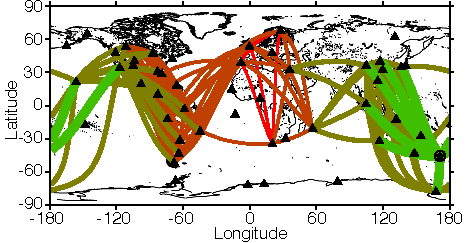
\includegraphics[scale=1]{energy/Figures/PPS_Hop.pdf}\\
\caption{An example of the bootstrapping technique, showing calibration distance from the main Dunedin station. Thick green lines are the first calibration stage and the thin red lines the last. Stations may be unconnected due to not having common strokes, being poor intermediary stations or being down for the day.}
\label{energy:fig:bootstrap}
\end{figure}

\subsection{Energy Calculation}

The fully calibrated WWLLN network is used to calculate the stroke energy for each station participating in a TOGA event using equation~\ref{energy:eq:power_eq} with the $A_{local}$ values known for a majority of the stations.
Of the participating stations, the median of their energy measurements is used as the final stroke value for the event.
The uncertainty in the energy is the median absolute deviation (MAD) of the participating station energy measurements, the MAD is the method of getting standard deviation of median values (MAD = median($|E_i - $median$(E_i)|$)).
On average 96.97\% of WWLLN strokes have an energy value, even with only an average of 2/3 of stations being well calibrated and participating in energy calculations.
The 3.03\% of strokes without energy values either were not reported by any well calibrated stations or had an uncertainty greater than 100\% in which case they are thrown out.

The last step in calculating the energy per stroke is an iterative technique to improve accuracy.
The first set of energy values are used as a basis to recalibrate all of the stations in the network.
These new values are used to recalibrate again with this process repeating several times until the station calibrations converge to a stable and final value.
Currently the station calibrations along with this iterative technique are performed once a day for calculating the stroke energies of that day.

The bootstrap method of calibration is an internally consistent method of determining the conversion factors at each station.
The iterative technique allows for a convergence of calibrations to reduce the uncertainty in the energy measurements.
Even the original calibrated station is updated in each iteration, removing errors that may be introduced by local effects since the initial ground truth calibration.
However the internal consistency could be improved and monitored through the introduction of a second well-calibrated station; such a station would enable additional diagnostics and error correction not possible with a single starting station.

\section{Results}

\subsection{Validation}

A study was conducted comparing the stroke energy values determined by WWLLN to the ground based NZLDN measurements of return stroke absolute peak current. NZLDN was described earlier by \citet{Rodger2006}.
The comparison was done using three periods of high lightning activity over New Zealand: 25 -- 27 August 2009, 26 -- 27 September 2009 and 21 October 2009.
WWLLN strokes were considered to match NZLDN strokes if they occurred within 0.5~ms and 400~km of a NZLDN detector, the same criteria used by \citet{Rodger2006}.
From the comparison the empirical relation between return stroke peak current and 6 -- 18~kHz RMS radiated energy was found to be: 

\begin{equation}
E_{stroke} = 2.23 * |I_{peak}|^{1.62}
\label{energy:eq:Peq}
\end{equation}

where $E_{stroke}$ has units of watts and $I_{peak}$ has units of kA.
In figure~\ref{energy:fig:pvi} the WWLLN peak current (using the inverse of equation~\ref{energy:eq:Peq}) is shown against the NZLDN absolute peak current.
When taking the uncertainties of the energy values (converted to peak current) and an assumed 30\% uncertainty in the NZLDN data, 84\% of the matched strokes have equivalent peak currents.
The peak current values fit close to the unity line with a robust linear fit of $I_{WWLLN}=0.93*I_{NZLDN}+1.93$ with an $R^2$ value of 0.92, a robust fit is used due to the lognormal behavior of the WWLLN power data.
Of the matched strokes 86.5\% are shown in figure~ \ref{energy:fig:pvi} with the remaining 13.5\% out of the plotted bounds.
This strong relationship confirms that the energy values measured are directly related to the physical properties of the stroke. i.e. the return stroke peak current.

\begin{figure}[ht!]
\centering
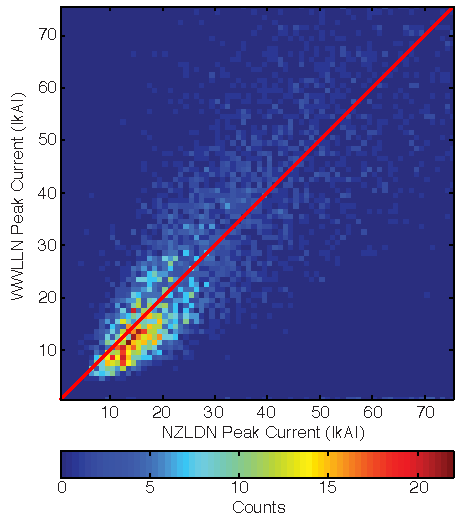
\includegraphics[scale=1]{energy/Figures/PPS_PvI_Error.pdf}\\
\caption{WWLLN peak current versus NZLDN return stroke peak current for three time periods in 2009 using 5260 matches. WWLLN peak current derived from $E_{stroke} = 2.23 * |I_{peak}|^{1.62}$, 84\% of strokes are within range of the unity line (red solid line) with uncertainty taken into account. 86.5\% of NZLDN-WWLLN matched strokes shown (others out of range).}
\label{energy:fig:pvi}
\end{figure}

\subsection{Error and Uncertainty}

The model used in relating the stroke energy to the peak current uses the 2010 average stroke uncertainty of 17\% from the median of the MAD distribution of all strokes in the year.
If a stroke has an uncertainty greater than 100\% that value is thrown out, doing so only decreases the number of stroke energies by 3.03\%.

The largest source of uncertainty in the calculations arises from the assumptions that are made using the LWPC code and in the calibration process.
The lookup tables used to calculate attenuation on a given stroke are gridded into $1^{\circ}$ by $1^{\circ}$ bins and averaged over the 8 -- 18~kHz frequency range.
This assumes that the attenuation rates do not vary greatly within a given grid and that the frequency spectra of a sferic is relatively flat within the band considered.
The ionospheric models used within the code assume a perfectly smooth day or night ionosphere, paths crossing the terminator are weighted averages of these values.
These issues arise from the inherent speed limitations of the LWPC code.

A secondary source of uncertainty manifests as variations in the WWLLN station calibration factors.
These are not caused by drift in the electronics, rather from variations in the local station environment and the ionosphere along the path.
Local weather could change the gain at a station (for example through water or ice on an antenna) or if there are significant changes in conductivity of the ground or ionosphere.
Since the LWPC code results are fixed, the only free variable in the bootstrapping process are the station conversion factors, so variations in the propagation path manifests within these factors.
These uncertainties are mitigated by performing a seven day running average of the calibration values but they are still present as daily variations in the calibrations.

Uncertainties that arise through the use of the LWPC model and through the station calibrations are seen through the MAD of each stroke.
Without these uncertainties each stations should agree on the detected stroke power, however the variations between each station, due to changes in the propagation path or in the calibration, appear as differences in reported stroke power.
Even with these differences the overall 17\% uncertainty of the WWLLN energy measurements is comparable to the 13\% uncertainty in the peak current measurements of the U.S. National Lightning Detection Network (NLDN) \citep{Nag2011}.

\section{Discussion}

\subsection{Comparison to Literature}

The current method of measuring stroke powers using WWLLN results in a consistent global median RMS power of 1.33 x $10^3$~J for 2010.
However it has been shown in past literature on radiated stroke power that the average is between $3\pm4$ x $10^9$~W and  $2\pm2$ x $10^{10}$~W \citep{Krider1983}.
A gain of 35 dB to 43 dB in power is needed to bring the WWLLN stroke powers into the range of those in the literature.
Three aspects of our measurement technique: peak vs RMS power, digital filtering, and the attenuation of the ground and sky wave near the stroke combine to explain this large difference in the scalable value of the reported stroke power.

The analysis of the difference was done using the raw waveform data from three stations: the secondary Seattle station, the Canaveral station and the Tallahassee station.
Data was taken from between 20 April 2011 and 9 May 2011. In this interval 198 events were selected that had a clear waveform at the network trigger time.

All of the measurements of power in the literature are measurements of peak power, however WWLLN is measuring RMS power.
The average peak value of the sferic waveforms, used in Figure~\ref{energy:fig:average_spectra}, is 8.8~dB greater than the RMS value of the waveform. 
Before the power value is computed at a WWLLN station the full waveform is sent through a 6 -- 18~kHz 16 point FIR bandpass filter.
This filter is used to cut out the strong signals from various high powered VLF communications transmitters.
While most of the VLF radiated power is in the 6 -- 18~kHz band, it is not a sharp cutoff.
This filtering of the waveform before calculating power causes a power reduction of 1.5~dB.

The biggest effect on the received stroke power is caused by the distances involved in the measurement and most particularly the differences between the ground and sky wave near the stroke and the waveguide propagated signal (and hence received powers).
Most of the VLF power measurements in the literature have measured waveforms at around 100~km from the stroke.
These distances are near enough that the ground and sky wave has not yet been attenuated by the structure of the Earth-ionosphere waveguide.

To measure the effect that the nearby high attenuation will have compared to a signal in the waveguide the difference in stroke power of the VLF transmitter near Seattle, NLK (250~kW radiated power at a frequency of 24.8~kHz, i.e. \citet{Clilverd2009}), was compared to the same signal seen at two stations in Florida.
A second transmitter in Hawaii, NPM (500~kW radiated power at a frequency of 21.4 kHz), was used as a reference for both stations.
The two Florida stations were chosen as they are far from both VLF transmitters and sample at a Nyquist frequency of 48~kHz, well above the frequencies of the lightning peak power and the VLF radio transmitter frequencies.

The LWPC code estimate for the transmitter signal at the WWLLN stations is compared to the measured transmitter signal to determine the conversion factor for each event.
The conversions are found to be consistent with calculations and calibrations reported in this study for broadband lightning produced signals.
Based on the verification of the LWPC code performed by \citet{Thomson2010}, LWPC is confidently used as a ground truth for this comparison.

The conversion factors from the NLK and NPM signals present in the selected waveforms were used to calculate the power of the two transmitters using the same method as the WWLLN power calculations.
To determine the importance of the ground wave, the ratio of estimated NLK to NPM powers at Seattle were divided by the NLK to NPM ratio at the two Florida stations.
This ratio is necessary, instead of just the Seattle NLK to actual NLK power ratio, in order to normalize out any intrinsic errors in the calculation process.
Measuring the waveguide signal causes a loss of 17.9~dB to 23.8~dB on the signal power as seen by WWLLN compared to the corresponding nearby ground and sky wave measurements.

These three factors show how 28.2 to 34.1~dB of power is lost from ground wave measurements to those made of the waveguide propagating fields by WWLLN, which is near the range of the 35 to 43~dB loss needed to explain the difference between the WWLLN and past power measurements.

This analysis leads to the conclusion that the power being measured by WWLLN is not the total radiated power of the stroke, rather it is the RMS power radiated into the Earth-ionosphere waveguide in the 6 -- 18~kHz band.

\subsection{Power Distribution}

Stroke power in a given thunderstorm, region or time span closely follows a lognormal distribution \citep{Golde1977}. Figure~\ref{energy:fig:distribution} shows the stroke power distribution for all strokes seen by WWLLN in 2010 along with the distributions for the three major chimney regions of the Americas, Africa/Europe and Asia/Australia.
The Americas and Asia/Australia show similar distributions, likely a result of having similar WWLLN coverage, while Africa/Europe differ, possibly due to uneven network coverage.


%% Remake with energy

\begin{figure}[ht!]
\centering
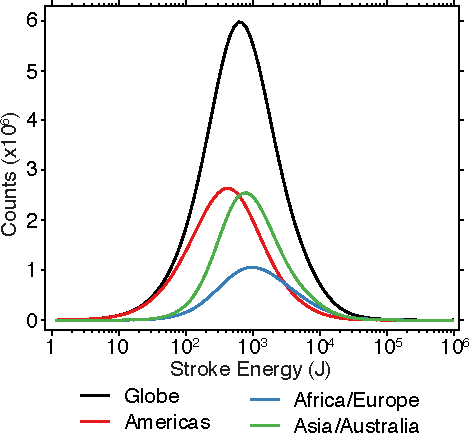
\includegraphics[scale=1]{energy/Figures/PPS_Distribution2.pdf}\\
\caption{Histogram of stroke powers for 2010 with 100 logarithmically spaced bins, the histogram for the globe (1.4 x 10$^8$ strokes) is shown in black, the Americas (6.1 x 10$^7$ strokes) in blue, Africa/Europe (2.4 x 10$^7$ strokes) in red and Asia/Australia (5.0 x 10$^7$ strokes) in green. Error bars are too small to display.}
\label{energy:fig:distribution}
\end{figure}
 
When the power distribution of figure~\ref{energy:fig:distribution} is converted to peak current using equation~\ref{energy:eq:Peq} it can be compared to earlier measurements of peak current distributions.
We can compare the WWLLN peak current distribution to that of \citet{Popolansky1972} as shown in \citet{Golde1977}.
That study used peak current data from 624~return strokes to create a cumulative probability distribution of stroke currents as shown in Figure~\ref{energy:fig:PPS_CDF}.
A similar frequency distribution was created using the WWLLN peak current estimates and is shown in the same figure.
As can be seen, the WWLLN distribution is shifted by a factor of two compared to the previous distribution, which is expected as WWLLN is known to detect higher current strokes when compared to what is seen by regional ground based networks \citep{Abarca2010}.
In a comparison to the NLDN those authors found that the probability distribution function of the WWLLN coincident strokes was similarly of an order two higher than the distribution for all NLDN strokes.
These comparisons further validate the stroke power to peak current relation of equation~\ref{energy:eq:Peq} and demonstrates this relationship is likely valid for the entire global network, and not just the New Zealand region.

%% Remake with stroke energy
\begin{figure}[ht!]
\centering
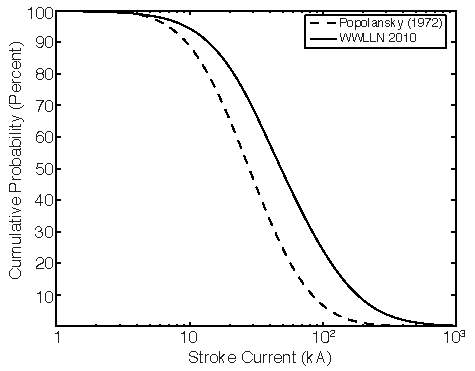
\includegraphics[scale=1]{energy/Figures/PPS_CDF.pdf}
\caption{The cumulative probability distributions of stroke current for the best fit of the \citet{Popolansky1972} data (dashed) and the 2010 WWLLN dataset (solid).}
\label{energy:fig:PPS_CDF}
\end{figure}

Africa has a lower detection efficiency in the network due to the small number of stations on the continent.
With a lower detection efficiency only the strongest strokes are seen by the more distant stations while the weaker strokes are not seen by these stations due to the stronger attenuation of VLF over continents than for propagation paths over water \citep{Wait1970}.
An initial effort to model the detection efficiency of WWLLN showed this effect very strongly (\citet{Rodger2006}, Fig. 11).
This results in the distribution of figure~\ref{energy:fig:distribution}, with fewer low powered strokes occurring over Africa compared to the other regions.

Without a full understanding of the regional detection efficiency of the network it cannot be determined whether every region follows the same lognormal power distribution or whether local environments affect the power of strokes in the region.
However, the bootstrap calibration process described in the current study may allow new estimates of the global variation in WWLLN detection efficiency, following \citet{Rodger2006}.

\section{Conclusion}

A new method of measuring the VLF waveguide mode power radiated from lightning using the WWLLN has been shown and validated.
While not the total radiated power of the strokes, the power measured is directly related to the peak current and therefore to inherent properties of the strokes.
Our study shows that WWLLN observations can provide realistic return stroke peak current measurements in addition to the timing and location of global lightning activity.

The method developed here can be applied to similar ground based lightning detection networks.
The key components in applying this method are the availability of a propagation model in the frequency range of the sensors (LWPC in the case of WWLLN), a measure of stroke strength (e.g. peak electric field), and at least one well-calibrated station.
Finally the station density needs to be high enough such that the average inter-station distance is within the applicable range of the propagation model used.

An enhanced WWLLN allows for a global real time view of lightning with the ability to distinguish between weak and strong strokes.
This will allow for future research into areas such as the long range evolution of thunderstorms over oceans, wider surveys of terrestrial gamma ray flashes, and with a more complete understanding of detection efficiency an analysis of global lightning power output.

\subsection*{Acknowledgments} 
We are grateful to the New Zealand MetService Ltd. for collecting the NZLDN data, and to Antarctica New Zealand for supporting the operation of the Scott Base WWLLN station.
This research in this chapter was supported in part by the National Science Foundation Grant \#AGS-0809988.


% ========== Chapter WWLLN Detection Efficiency

\chapter{WWLLN Detection Efficiency}
\label{thesis:chapter:efficiency}

%% Overall change tense as needed

\section{Overview}

%% Merge abstract and introduction together

Using the detected energy per strokes of the World Wide Lightning Location Network (WWLLN) we calculate the relative detection efficiency for the network as if it had a uniform  detection efficiency.
The model uses the energy statistics of located strokes to determine which stations are sensitive to what stroke energies.
We are then able to estimate the number of strokes that may be missing from any given regions as compared to the best, most sensitive regions of the WWLLN network.
Stroke density maps can be corrected with the knowledge of how sensitive various regions of the network are operating.

This new model for the relative WWLLN detection efficiency compensates for the uneven global coverage of the network sensors as well as variations in very low frequency (VLF) propagation.
The model gives a way to represent the global distribution of strokes as if observed by a globally uniform network.
The model results are analyzed in spatial and temporal regimes, and the effects of a single VLF detector going offline are investigated in areas of sparse and dense detector coverage.
The results are also used to show spatial, temporal and energy distributions as seen by the detection efficiency corrected WWLLN.

%% Better transition
However the WWLLN network does not observe lightning with the same detection efficiency everywhere.
This is due to variable WWLLN station coverage and the strong affect on very low frequency (VLF) radio propagation from orography and ionospheric conditions along the great circle path of a wave.
This paper demonstrates a technique which uses only data collected by the WWLLN network itself, to estimate the relative detection efficiency of each $5^\circ$ x $5^\circ$ pixel over the earth compared to the best average WWLLN detection efficiency.
For instance, the lightning stroke density over central Africa, where WWLLN station density is sparse, can now be compared to the region of the Earth with the best detection efficiency, such as North America.
This chapter does not provide an absolute detection efficiency calculation.

A concern for all VLF networks is the non-uniform propagation of VLF waves due to changing ionospheric  and surface conditions; this is true for networks monitoring lightning produced VLF signals like WWLLN, or those monitoring fixed-frequency communication transmitters like AARDDVARK \citep{Clilverd2009}.
During the day there is a larger ionospheric electron density at lower D-region altitudes.
This causes the range of electron-neutral collision frequencies to overlap with the range of sferic wave frequencies, increasing the attenuation rate of the sferics.
This increase in electron number density is also seen in the change of the reference ionospheric height, $h'$ \citep{Wait1960a}, during the day ($h'=74$~km) compared to during the night ($h'=87$~km).
There is a similar change in attenuation over the path of the sferic from the differences in the conductivity of the oceans (4~S/m), continents ($10^{-2}$~-- $10^{-4}$~S/m), and Antarctic/Arctic ice ($10^{-5}$~S/m).
The many path parameters for a given sferic result in a highly variable attenuation \citep{Volland1995}.

Thus, independently determining the real-time detection efficiency has always been a challenging topic.
Several studies have been conducted comparing the network to other ground based networks or satellite measurements \citep{Lay2004b, Jacobson2006c, Rodger2009, Abarca2010, Abreu2010}.
These studies tend to be limited in either scope or in time due to the availability of data from other networks.
Past work by \citet{Rodger2006} attempted to determine the global detection efficiency of WWLLN using a theoretical model linked to observations from a ground based commercial lightning network in New Zealand.
In this paper a new method is developed for determining  the relative detection efficiency of WWLLN based upon the recent network advancement of measuring the radiated energy of detected strokes \citep{Hutchins2012}.

Developing a model of detection efficiency expands the capabilities and uses for WWLLN.
In particular a model that does not rely on external comparisons to other networks or sensors is critical for obtaining a dynamic global view of network performance.
Such a view will enable the network to be used with more confidence in areas of lower coverage and enable the network to be utilized with uniform detection efficiency in work requiring lightning rates and densities.
This uniform performance will allow for more accurate studies of global phenomena such as the short time ($<$10 minute) variability of the global electric circuit, comparative lightning climatology between regions, and production rate estimations of transient luminous events and terrestrial gamma ray flashes.
The detection efficiency model can combine with the measurements of stroke energy and regional absolute detection efficiency studies to advance research in global effects of lightning such as estimating the total sferic energy transferred to the magnetosphere in the form of whistler waves.

\subsection{Calculating the Radiated Stroke Energy}

Every WWLLN sferic packet includes the TOGA and a measure of the root mean square (RMS) electric field of the triggered waveform.
The RMS electric field is taken in the 6-18~kHz band over the triggering window of 1.33~ms.
The U.S. Navy Long Wave Propagation Capability (LWPC) code described by \citet{Ferguson1998} is utilized to model the VLF propagation from each located stroke to determine the necessary stroke energy to produce the measured RMS electric field (in the VLF band) at each WWLLN station.
Using the measured RMS field at each station, the radiated energy of each detected stroke is found.
In 2010 WWLLN observed a global median stroke energy of 629 J, with a 25\% average uncertainty in the measured energy.
The global and regional distribution of energy is shown in Figure~\ref{efficiency:fig:2010_Energy}a.
Of all the detected strokes 97\% have corresponding energy values.
\citep{Hutchins2012}

\begin{figure}[ht!]
   \centering
\noindent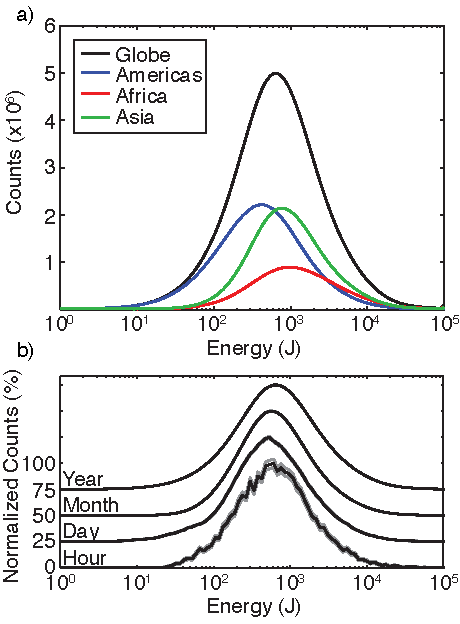
\includegraphics[width=20pc]{efficiency/Figures/2012RS005049-p1.pdf}
   \caption{(a) WWLLN stroke energy distribution for the globe (black), the Americas (blue), Asia (green) and Aftica/Europe(red).
(b) WWLLN global stroke energy distribution for a year (2010), month (June 2010), day (15 June 2010), and hour (09 UTC 15 June 2010).
Grey lines are statistical count errors.}
   \label{efficiency:fig:2010_Energy}
\end{figure}

In Figure~\ref{efficiency:fig:2010_Energy}a the statistical error bars (Poisson statistics) are not plotted as they would be on the order, or smaller than, the line width.
It is important to note that the distribution of strokes in each region is lognormal \citep{Hutchins2012} with the main differences in the total strokes detected and the median energy, which is 399~J, 1101~J, and 798~J for the Americas ($-180^\circ$ E to $-60^\circ$ E), Africa ($-60^\circ$ E to $60^\circ$ E), and Asia ($60^\circ$ E to $180^\circ$ E) respectively.
An overall lower detection efficiency over Africa, particularly for low energy strokes, causes median energy to be higher than the other regions.
Along with each region the energy distribution is lognormal from an hourly time scale to the annual distribution.
In Figure~\ref{efficiency:fig:2010_Energy}b the annual lognormal distribution is shown with a monthly, daily, and hourly distribution.
It is not until the hourly distribution that the errors are noticeable, and the distribution is still fairly lognormal.

\section{Minimum Detectable Energy}

The first step in calculating the relative detection efficiency for the entire network is working out the minimum stroke energy that WWLLN can detect at a given location and time.
This process starts by finding the detection threshold at each station, converting it to an energy value at each location in the world, and then selecting the minimum detectable network energy at every location based on the minimum observable energy from each station.
Detailed examples of how this works are given next for single stations and for the network as a whole.

\subsection{Station Threshold}

At each WWLLN station the threshold for triggering on an event (and calculating the TOGA at that station) is dynamically selected depending on observed activity at that station as described in Section 5.3 of \citet{Rodger2006}.
Presently every WWLLN station automatically adjusts the triggering threshold to send an average of 3 packets per second to the central processor.
For instance, when a station is detecting many strokes, the trigger threshold at that station is raised to maintain a steady flow of sferic packets.
Since a station can only measure the electric (or magnetic) field of an event it cannot accurately discern whether a sferic comes from a nearby weak stroke or a strong distant stroke; for the case of the strongest lightning strokes the discharge could be on the other side of the Earth from the WWLLN station and still be detected.


The effect of the variable trigger threshold can be seen in Figure~\ref{efficiency:fig:Threshold}a which is a 2~-~D histogram of number of strokes with specific RMS field and UT values on 15 June 2010 for the Dunedin, New Zealand, WWLLN station ($-45.864^\circ$ N, $170.514^\circ$ E).
In Figure~\ref{efficiency:fig:Threshold}b the threshold can be seen as the lower cutoff of the triggered RMS field strength distribution, the station threshold is reconstructed hourly as the 5th percentile value (red line) of the distribution.
The threshold value varies relatively slowly over the course of the day.


\begin{figure}[ht!]
   \centering
\noindent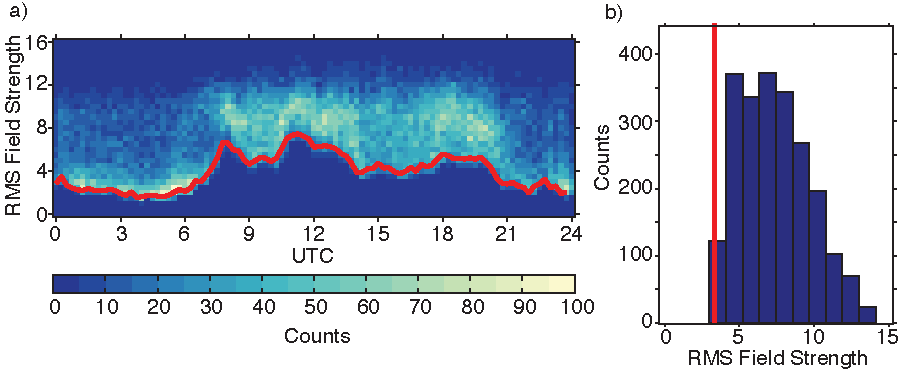
\includegraphics[width=39pc]{efficiency/Figures/2012RS005049-p2.pdf}
   \caption{(a) shows the evolution of the triggered RMS field strength distribution (in arbitrary units) for the Dunedin WWLLN station with the red line showing the 5th percentile value.
(b) shows the 9 UTC slice of the distribution, with the 5th percentile value marked (red line).}
   \label{efficiency:fig:Threshold}
\end{figure}

\subsection{Station Minimum Detectable Energy}

The minimum detectable energy (MDE) is the minimum energy a lightning stroke must radiate in the VLF to be detected by WWLLN or a WWLLN station (denoted network MDE and station MDE respectively).
The MDE is a function of space, time and station threshold.
Each station has a variable threshold which varies slowly during the day.
Slow ionospheric variations can also affect the MDE by changing the VLF attenuation and detected RMS field.


Every hour the reconstructed minimum RMS field necessary to trigger an event is calculated and converted to a stroke energy.
To make this conversion the same method as calculating the radiated energy per stroke is used as described in \citet{Hutchins2012}.
This results in a station MDE for every point on a $5^\circ$ x $5^\circ$ global grid, which is the stroke energy necessary at that location to trigger a TOGA calculation at the given station.
As an example the map of the MDE for our Dunedin station (data shown in Figure~\ref{efficiency:fig:Threshold}) is shown in Figure~\ref{efficiency:fig:Threshold_Map}.
Figure~\ref{efficiency:fig:Threshold_Map} applies only to strokes detected at this one station in Dunedin, a similar map can be generated for every WWLLN station.
The high MDEs in Figure~\ref{efficiency:fig:Threshold_Map} over the Antarctic, Western Africa, and Greenland are due to the high VLF attenuation over ice, and imply that Dunedin is very unlikely to detect strokes with energy less than the MDE if they were to occur in these regions.

\begin{figure}[ht!]
   \centering
\noindent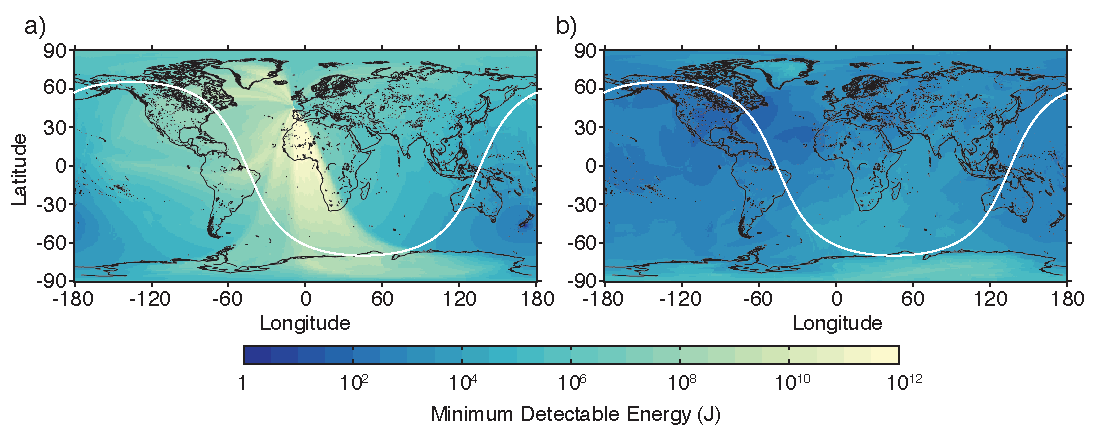
\includegraphics[width=20pc]{efficiency/Figures/2012RS005049-p3.pdf}
   \caption{The minimum detectable energy (MDE) for the Dunedin station at 9 UTC on 15 June 2010.
The regions of high MDE are due to poor VLF propagation over ice from those regions to Dunedin station.
The white line shows the terminator.}
   \label{efficiency:fig:Threshold_Map}
\end{figure}

In order to locate a stroke, WWLLN requires TOGA values from at least five stations in order to conduct adequate fit error analysis.
For every $5^\circ$ x $5^\circ$ grid cell all of the minimum stroke energies from currently active WWLLN stations are ordered.
An example for one cell is shown in Table~\ref{efficiency:table:mdeTable}.
The 5th lowest from this list is used as the network MDE, because at least five stations can trigger on that energy value.
In other words, WWLLN cannot detect a stroke until it has a radiated energy which is above the trigger threshold at five or more WWLLN stations.
A map of the network MDE is shown in Figure~\ref{efficiency:fig:Minimum_Energy}.
Similar to the station MDE map for our Dunedin station, Figure~\ref{efficiency:fig:Threshold_Map}, there are higher MDE values above the Arctic and Antarctic ice regions.

\begin{table}[ht!]
\caption{Ordered list of station MDE values at $-25^\circ$N, $20^\circ$E and 09 UTC on 15 June 2010.
The fifth lowest value (in bold) is the network MDE at this location.}
\begin{center}
\begin{tabular}{p{2in}p{1in}}
\hline
Station Name 		& 	MDE (J)\\
\hline
\rule{0pt}{3ex}
Davis, Antarctica	&	34.5\\
Ascension Island	&	169.2\\
SANAE Base, Antarctica	&	193.9\\
Perth, Australia	&	2268.3\\
{\bf Rothera, Antarctica}	&	{\bf 2413.5}\\
Tel Aviv, Isreal	&	4701.1\\
. . .	&	. . .\\
Honolulu, Hawaii	&	$1.35 \times 10^8$\\
Dunedin, New Zealand	&	$5.09 \times 10^8$\\
\hline
\end{tabular}
\end{center}
\label{efficiency:table:mdeTable}
\end{table}

\begin{figure}[ht!]
   \centering
\noindent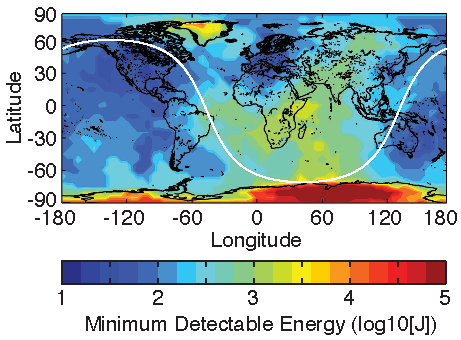
\includegraphics[width=20pc]{efficiency/Figures/2012RS005049-p4.pdf}
   \caption{The minimum detectable energy (MDE) for the entire WWLLN network at 9 UTC on 15 June 2010.}
   \label{efficiency:fig:Minimum_Energy}
\end{figure}

Regions of the network with higher MDE, from either increased VLF attenuation, station thresholds or sparse coverage, preferentially detect a higher ratio of energetic strokes to all strokes.
For example southern Africa has a higher MDE than other regions and the median energy, shown in Figure~\ref{efficiency:fig:2010_Energy}a is correspondingly higher.
Conversely regions with low MDE, such as the Americas, show a lower median energy.

\section{Relative Detection Efficiency}

The next important step in calculating the relative detection efficiency is to establish the relationship between the network MDE and relative detection efficiency.
The relative detection efficiency is a measure of how well a given location in the network is being observed relative to the best region in the network.
In a given grid cell the network MDE is compared to the total WWLLN energy distribution of the past seven days.
For a given network MDE value the fraction of total strokes above the network MDE gives the relative detection efficiency.
The past seven day distribution is used as the base distribution in order to average over diurnal and station performance variations.
This lognormal base distribution is assumed to be representative of a single universal distribution of stroke energies that could be detected globally by a uniform WWLLN.

For example, if a location has an network MDE of 100~J, then the number of strokes in the past seven days above 100~J (grey area, Figure~\ref{efficiency:fig:Curve}a) is compared to the total number of strokes which were located in that location in those seven days.
In this case the grey area has a count of $2.6\times10^6$ strokes and the total number of WWLLN strokes is $2.9\times10^6$ strokes, so for this network MDE of 100~J the relative detection efficiency is 90\%.
Similarly if a location has a high network MDE value there will be few strokes with energy above it, so it will have a low relative detection efficiency.

\begin{figure}[ht!]
   \centering
\noindent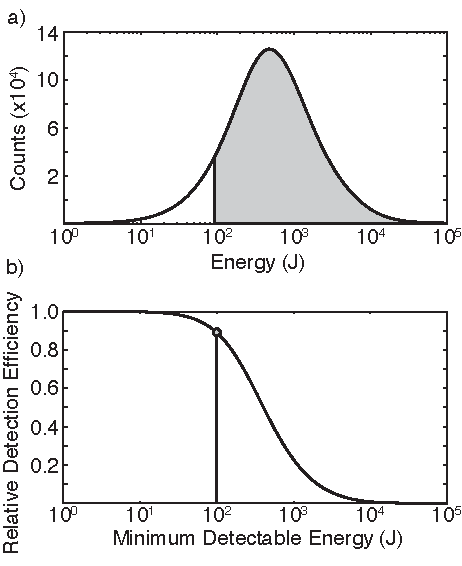
\includegraphics[width=20pc]{efficiency/Figures/2012RS005049-f5.pdf}
   \caption{(a) The seven day energy distribution with the strokes above the MDE of 100~J shown in grey.
The fraction of strokes above 100~J to total strokes gives a relative detection efficiency of 0.9, shown as a circle in (b).
The fraction for all possible MDE values is shown as the curve in (b).}
   \label{efficiency:fig:Curve}
\end{figure}

This calculation is done for a range of hypothetical network MDE values which produces a curve shown in Figure~\ref{efficiency:fig:Curve}b, to give the relationship between MDE and relative detection efficiency.
This relationship is established once per day, and it is used to produce hourly maps of relative detection efficiency for that day.
This is done by taking the hourly maps of network MDE and applying this relation to every $5^\circ$ x $5^\circ$ point on the globe for every hour to convert the network MDE to the relative detection efficiency.

The relative detection values given by this process are only in reference to the energy distribution of the past seven days as seen by WWLLN.
If a region has a relative detection efficiency of 100\% then the region is able to detect all of the detected stroke energies present in the 7-day network energy distribution.
The corrections from the relative detection efficiency maps can be used to generate lightning density distributions as though WWLLN had global uniform coverage at the same level as that of the best parts of the network.
This is because the method does not correct the network to absolute stroke counts, just to a globally uniform performing WWLLN.

\subsection{Hourly Maps}

A set of four hourly maps from 15 June 2010 showing the networks relative detection efficiency every 6 hours from 00~UTC to 18~UTC is presented in Figure~\ref{efficiency:fig:Hour_Maps}.
Stations that were operational for the hour shown are displayed in white and stations that were not operational are black (operational taken to triggering $>500$ strokes/hour).
The four major competing effects on the detection efficiency are the day/night terminator, local stroke activity, station density, and station performance.
The day/night terminator effect can be seen as it moves from 00~UTC (Figure~\ref{efficiency:fig:Hour_Maps}a) through 18~UTC (Figure~\ref{efficiency:fig:Hour_Maps}d).
An increase in local stroke activity in North American afternoon (Figure~\ref{efficiency:fig:Hour_Maps}a) causes a decrease in detection efficiency as nearby stations raise their triggering thresholds.
Station density is coupled with station performance, since when a station is not operating optimally it has a similar effect as removing that station, the effect of station performance is discussed in a later section.

\begin{figure}[ht!]
   \centering
\noindent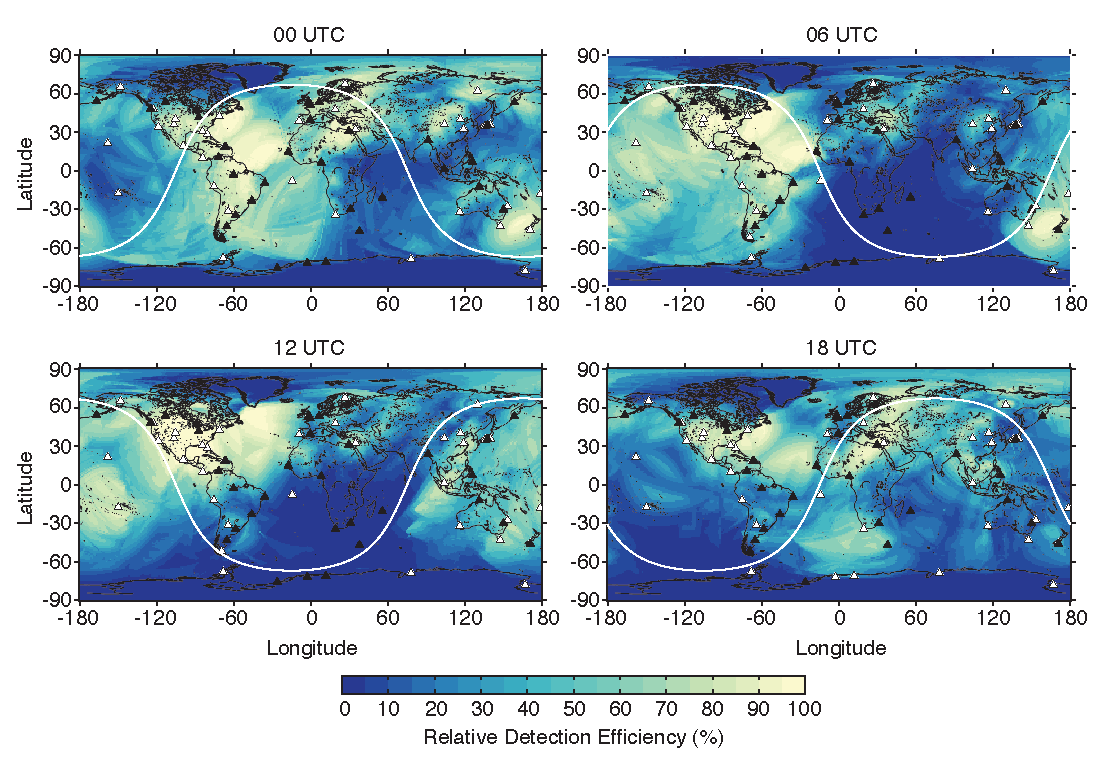
\includegraphics[width=39pc]{efficiency/Figures/2012RS005049-p6.pdf}
   \caption{Relative detection efficiency maps for 00, 06, 12, and 18 UTC on 15 June 2010.
Stations are shown as triangles with operational stations in white and non-operational in black.
The minimum value of detection efficiency is set at 5\% to prevent unphysical corrections.}
   \label{efficiency:fig:Hour_Maps}
\end{figure}

Figure~\ref{efficiency:fig:Daily_Map} shows the daily relative detection efficiency from the average of the hourly maps, here grey stations were only operational part of the day.
This average map is more representative of the relative detection efficiency for the day and it shows behavior that is expected based on the distribution of stations: lower detection efficiency over most of Africa with higher detection efficiency over and around the Pacific and North America.
The low detection efficiency over Antarctica, parts of Siberia, and Greenland are due to the high attenuation of VLF propagating subionospherically over ice.
Conversely the high detection efficiency over North America, Western Europe, and Oceania, are due to the high station density and low attenuation of VLF over ocean.
In order to prevent unphysical overcorrections, a minimum relative detection efficiency of 5\% has been set for all of the relative detection efficiency maps.

\begin{figure}[ht!]
   \centering
\noindent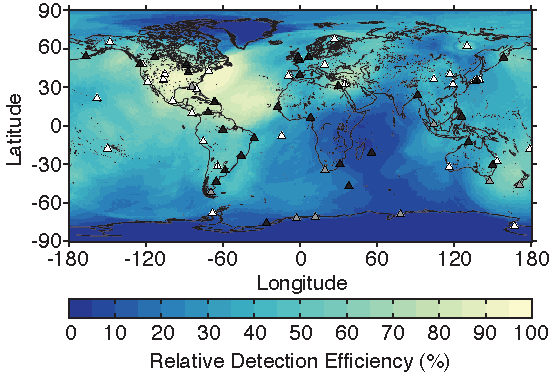
\includegraphics[width=20pc]{efficiency/Figures/2012RS005049-p7.pdf}
   \caption{Daily average relative detection efficiency for 15 June 2010.
Stations are shown as triangles with operational stations in white, non operational in black, and operational for part of the day in grey.
The minimum value of detection efficiency is set at 5\% to prevent unphysical corrections.}
   \label{efficiency:fig:Daily_Map}
\end{figure}

\section{Analysis}

\subsection{Distribution Changes}

As shown in the previous sections the relative detection efficiency values in a given day are derived from the WWLLN observed stroke energy distribution from the previous seven days, this allows for direct comparisons within a day and for nearby days, but it does not take into account the changing distribution from changes in the network.
As more stations are added to the network additional low-energy strokes will be detected and the overall energy distribution will shift towards lower values.
When the overall network distribution changes between years, then for a given region the relative detection efficiency can change even if that region of the network has detected the same distribution of strokes.


One way to examine the change in the distribution of energy is to examine the temporal variability of the median of the global WWLLN energy distribution, the median of the seven day distribution is shown in Figure~\ref{efficiency:fig:MedianEnergy}.
The median energy varies from the three year median by 52\% with the daily median value ranging from 400~J to 2000~J.
The variability is caused by ionospheric changes not accounted for in the ionospheric model used.
Several jumps in the median energy (e.g., Dec 2009 and Dec 2010) are caused by changes in the primary calibrated WWLLN station (see \citet{Hutchins2012}) such as gain changes.
The slow increase to Aug 2011 was due to a change of the primary calibrated station from the Dunedin, New Zealand station to the Scott Base, Antarctica station.
It is important to note that since the detection efficiency is relative to the past seven days, the relatively slow changes in median energy do not strongly affect the detection efficiency and highlight how the relative detection efficiency cannot correct for absolute overall network performance.

\begin{figure}[ht!]
   \centering
\noindent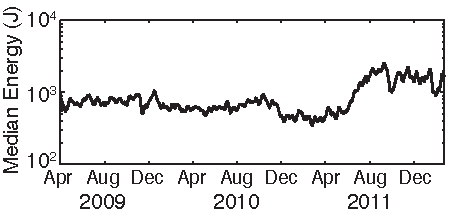
\includegraphics[width=20pc]{efficiency/Figures/2012RS005049-f8.pdf}
   \caption{Median stroke energy of the 7-day distribution observed by WWLLN.
The relative detection efficiency of the network is based on this 7-day energy distribution.}
   \label{efficiency:fig:MedianEnergy}
\end{figure}

\subsection{Temporal Variability}

The evolution of the network can be seen as an increase in the global average relative detection efficiency, calculated by averaging all grid cells of the each hourly maps for a day.
While no region can have a relative detection efficiency over 100\%, as regions improve with more stations they will approach 100\% and increase the global average detection efficiency.
The global average relative detection efficiency from April 2009 through October 2011 is shown as the green line in Figure~\ref{efficiency:fig:DE_Evolution}.
In the Figure the total number of operational stations is shown as the black line, and it has a strong correlation to the global averaged detection efficiency with a correlation value of 0.86.
With more stations strategically added to the network the 7-day energy distribution will also change to include more low energy strokes and increase the average relative detection efficiency.


\begin{figure}[ht!]
   \centering
\noindent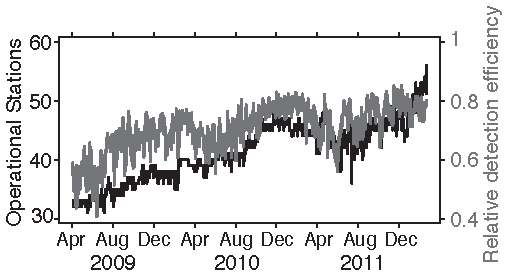
\includegraphics[width=20pc]{efficiency/Figures/2012RS005049-p9.pdf}
   \caption{The number of WWLLN stations operating (black) and the global average relative detection efficiency (green) for April 2009 through October 2011.}
   \label{efficiency:fig:DE_Evolution}
\end{figure}

While Figure~\ref{efficiency:fig:DE_Evolution} shows an overall increase in the number of network stations and hence detection efficiency, Figure~\ref{efficiency:fig:deTrendLocal} shows similar curves for just low-latitude regions ($-30^\circ$ N to $30^\circ$ N, blue), a single location near Florida ($-85^\circ$E, $30^\circ$N, red), and a single location near South Africa ($25^\circ$E, $-20^\circ$N, green).
Removing high latitude regions increases the overall detection efficiency but does not change the overall upward trend shown by the blue curve in Figure~\ref{efficiency:fig:deTrendLocal}.
When the region near Florida is examined it can be seen that it remains fairly close to 1.0 for the entire dataset, with downward trends during local summer months due to increased local lightning activity.
The region near South Africa has a steady increase in detection efficiency except during a large drop out which occurred in the middle of 2011, caused by one of the African stations going offline.
This shows the global detection efficiency tracks the network as a whole, but it cannot be used as an accurate proxy for smaller spatial scales.

\begin{figure}[ht!]
   \centering
\noindent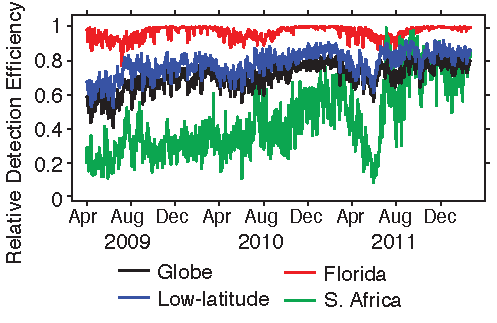
\includegraphics[width=20pc]{efficiency/Figures/2012RS005049-p10.pdf}
   \caption{Daily variation of average detection efficiency for the globe (black), low-latitudes ($-30^\circ$ N to $30^\circ$ N, blue), over Florida ($-85^\circ$E, $30^\circ$N, red), and over South Africa ($-25^\circ$E, $-20^\circ$N, green).}
   \label{efficiency:fig:deTrendLocal}
\end{figure}

The local time variability over the region near Florida is shown in black in Figure~\ref{efficiency:fig:deUTC} and shows a total variability of about 4.9\%.
The largest drop in the relative detection efficiency occurs in the afternoon, near the peak in local lightning activity at 3pm.
This drop is due to the nearby stations raising their detection threshold in response to detecting more local strokes.
For this location the effects of local activity dominates over the expected day/night effect due to changes in VLF propagation.

\begin{figure}[ht!]
   \centering
\noindent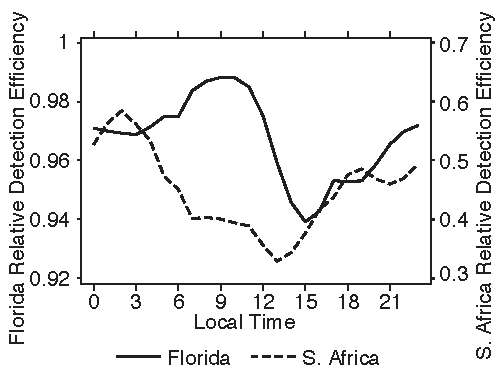
\includegraphics[width=20pc]{efficiency/Figures/2012RS005049-f11.pdf}
   \caption{Average local time variation of detection efficiency over Florida ($-85^\circ$E, $30^\circ$N, solid) and South Africa ($-25^\circ$E, $-20^\circ$N, dashed), from 2009-2011.}
   \label{efficiency:fig:deUTC}
\end{figure}

The variability for the region near South Africa is shown as the dotted line in Figure~\ref{efficiency:fig:deUTC}, there is a total variability of 25.5\%.
There is an overall decrease in relative the detection efficiency during the day when the sferics are propagating over the continent.
The best in relative detection efficiency occurs in the middle of the night when the stations in Africa have less nearby activity and sferics are able to propagate more readily under a night ionosphere.
Compared to the Florida region there is a much higher dependence on day and night conditions as well as a much wider range of variability.

\subsection{Station Outage Effects}

While the overall performance of the network trends along with the total number of stations, the effects  a single station turning on or off can have an effect on a large region of the global but only small effect on the network as a whole.
To test the influence of single stations a day of data was randomly selected, 16 June 2010, and the entire data were reprocessed with just the Honolulu, Hawaii station ($-158^\circ$E, $21^\circ$N) removed from the raw data and again with just the Maitri, Antarctica station ($12^\circ$E, $-71^\circ$N) removed.
The maps of the daily average with and without these stations are shown in Figure~\ref{efficiency:fig:scrubMap}.
For Hawaii the change is fairly local to its region in the Northeast Pacific Ocean, but leads to little effect across the entire network.
In the case of Maitri there is a larger effect since it is located in a region of sparse detector coverage and covers much of the southern Atlantic.

\begin{figure}[ht!]
   \centering
\noindent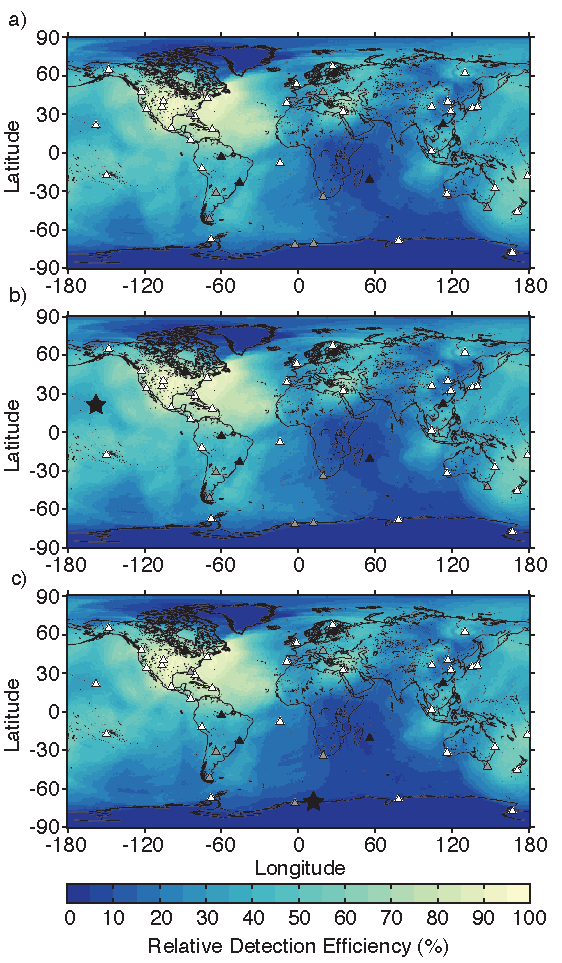
\includegraphics[width=20pc]{efficiency/Figures/2012RS005049-p12.pdf}
   \caption{Relative detection efficiency map of 16 June 2010  for (a) the complete network, (b) the network with the Hawaii station (black star, $-158^\circ$E, $21^\circ$N) removed, and (c) the network with Maitri station (black star, $12^\circ$E, $-71^\circ$N) removed.
Stations are shown as triangles with operational stations in white, non operational in black, and operational for part of the day in grey.}
   \label{efficiency:fig:scrubMap}
\end{figure}

The daily average global relative detection efficiency dropped from 64\% to 63\% without Hawaii and from 64\% to 53\% without Maitri.
The detection efficiency in the grid cell over Hawaii dropped from 85\% to 78\% and from 45\% to 7.4\% in the grid cell over Maitri.
A plot of the total change between the daily averages in Figure~\ref{efficiency:fig:scrubMap} is shown in Figure~\ref{efficiency:fig:scrub}.


\begin{figure}[ht!]
   \centering
\noindent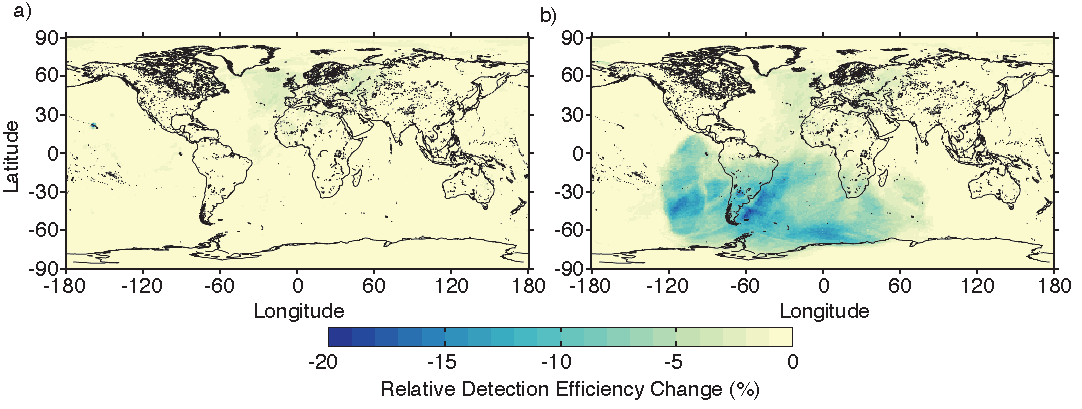
\includegraphics[width=39pc]{efficiency/Figures/2012RS005049-p13.pdf}
\caption{The difference in detection efficiency for 16 June 2010 with Hawaii (a) and Maitri (b) stations completely removed from processing.}
\label{efficiency:fig:scrub}
\end{figure}

\section{Results}

The detection efficiency model can be applied to global maps of stroke density to estimate, or correct for the global stroke density which would be seen if WWLLN had a uniform spatial and temporal coverage.
This does not correct for the overall absolute detection efficiency (11\% for CG flashes in the United States, see \citet{Abarca2010}), rather it corrects for the areas with less WWLLN coverage.
The hourly stroke density plots are corrected by dividing the counts in each grid cell by the relative detection efficiency of that cell.
For example a grid cell with 100 strokes and an efficiency of 80\% would be corrected to 125 strokes.
The stroke density from 2011, Figure~\ref{efficiency:fig:Global2011}, had the model corrections applied hourly with the condition that a 5$^\circ$ x 5$^\circ$ grid cell needed at least two strokes to have a correction applied.
A second condition was that a minimum relative detection efficiency of 5\% was set for the model.

\begin{figure}[ht!]
   \centering
\noindent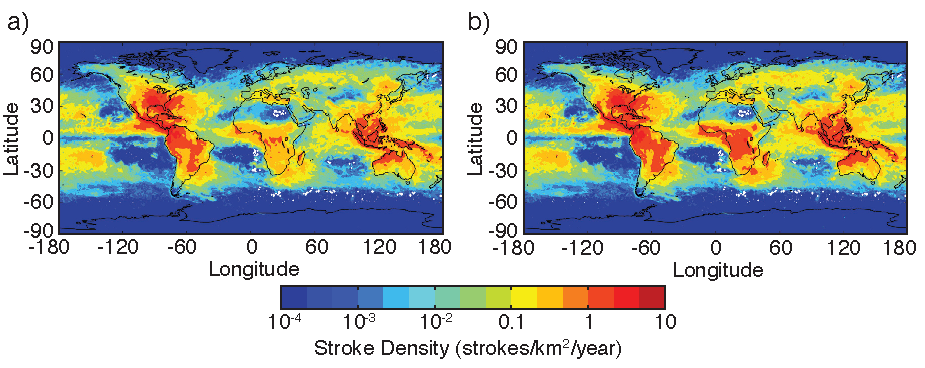
\includegraphics[width=20pc]{efficiency/Figures/2012RS005049-p14.pdf}
   \caption{The raw 2011 global stroke density measured by WWLLN.}
   \label{efficiency:fig:Global2011}
\end{figure}

The total number of strokes for 2010 was $1.4\times10^8$ (4.4 strokes/second), and after applying the model the total was $2.0\times10^8$ strokes (6.3 strokes/second).
In 2011 the total number of strokes was $1.5\times10^8$ (4.8 strokes/second) with a model-corrected value of $1.9\times10^8$ (6.0 strokes/second).
In 2010 63\% of the global area between $\pm60^\circ$ latitude had a relative detection efficiency of at least 80\% and in 2011 this area increased from 66\% to 72\%.
If we assume that the global lightning flash rate was a constant 46 flashes/second as determined by satellite measurements using the Optical Transient Detector and Lightning Imaging Sensor \citep{Cecil2011, Christian2003} for both years, this would imply a corrected global absolute detection efficiency for cloud to ground and in-cloud flashes of 13.7\% for 2010 and 13.0\% in 2011.

The corrected yearly density is shown in Figure~\ref{efficiency:fig:Global2011Corrected}, aside from the overall increase in number counts the important feature is the relative count rates over the US, Africa, and Southeast Asia.
In the uncorrected Figure~\ref{efficiency:fig:Global2011} the peak stroke density in Asia and America are similar while Africa is about $\sim$1-10\% of these values (also shown in Figure~\ref{efficiency:fig:2010_Energy}a).
In the corrected maps we can see that the peak density in Africa is much closer in magnitude to that seen for America and Asia, and the relative densities match the distributions seen by OTD (see \citet{Christian2003} Figure 4).
The total increase in stroke counts is shown in Figure~\ref{efficiency:fig:Global2011Diff} with the greatest increases occurring over land, in particular central Africa.

\begin{figure}[ht!]
   \centering
\noindent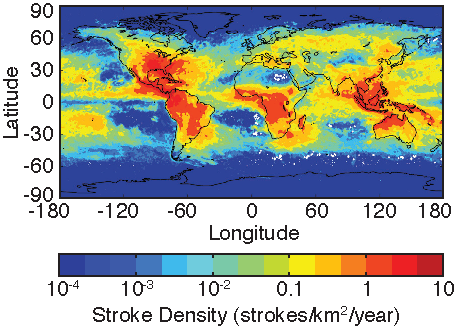
\includegraphics[width=20pc]{efficiency/Figures/2012RS005049-p15.pdf}
   \caption{The 2011 global stroke density measured by WWLLN and corrected for the relative detection efficiency of the network.
Note the large change in the African continent relative to Figure~\ref{efficiency:fig:Global2011}.}
   \label{efficiency:fig:Global2011Corrected}
\end{figure}

\begin{figure}[ht!]
   \centering
\noindent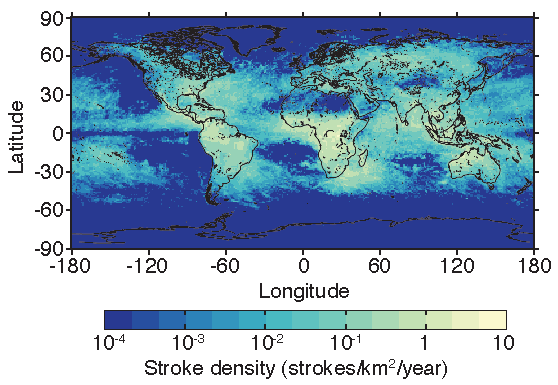
\includegraphics[width=20pc]{efficiency/Figures/2012RS005049-p16.pdf}
   \caption{The increase in stroke density due to the relative detection efficiency corrections for 2011.
Uncorrected and corrected stroke densities shown in Figure~\ref{efficiency:fig:Global2011} and~\ref{efficiency:fig:Global2011Corrected} respectively.
The increase is plotted on the same scale as the previous two figures.}
   \label{efficiency:fig:Global2011Diff}
\end{figure}

\section{Conclusion}

A relative detection efficiency model is developed for WWLLN based on the WWLLN observed stroke energy distribution.
The model is examined on various temporal scales as well as performance changes due to station outage effects.
The model is applied to the 2011 WWLLN dataset to produce a corrected map of stroke activity, matching the expected characteristics of satellite data.
Work on comparing distant regions is now possible as the network data can be corrected to a uniform global level of performance.
Future work will focus on achieving a model for absolute detection efficiency.


% ========== Chapter ENTLN-LIS Detection Efficiency

\chapter{ENTLN-LIS Detection Efficiency}
\label{thesis:chapter:entln-lis}

\section{Overview}

Performance of the Earth Networks Total Lightning Network (ENTLN) is evaluated with respect to the TRMM Lightning Imaging Sensor (LIS).
ENTLN lightning strokes are matched to LIS lightning flashes from 2011 -- 2013 over the continental United States and within the 35$^\circ$ orbital inclination of LIS.
ENTLN matched $1.4\times10^5$ of the $2.1\times10^5$ LIS flashes with a total of $4.8\times10^5$ strokes, giving an average multiplicity of 3.5 and 66\% detection efficiency of all flashes; over the course of the evaluation period the average daily detection efficiency was $69\pm14$\%.
The median timing offset from the first ENTLN stroke was 2.4~ms (LIS leading) with a sharp peak at -1.9~ms; the median distance offset was 7.0~km from the flash centroid.
The sharp peak at -1.9~ms is likely caused by inherent differences in the detection techniques: LIS observes light emitted from the tops of the clouds and ENTLN measures the radio signals from the return stroke.

The performance of LIS relative to ENTLN is also evaluated by finding all ENTLN strokes located within the LIS field of view.
LIS matched 68\% of the $7.1\times10^5$ ENTLN strokes in the LIS field of view.
The $70 \pm 12$\% daily average LIS detection efficiency of ENTLN strokes demonstrates that neither system detects every flash or stroke located by the other.
Assuming a 3.5 multiplicity of ENTLN unmatched strokes, LIS did not detect $6.6\times10^4$ flashes, or 31\% of all flashes.
The ENTLN-LIS matched strokes were $20.3 \pm 0.6$\% cloud to ground and unmatched strokes were $21.8 \pm 0.8$\% cloud to ground.
There is a marginal difference in the lightning populations sampled by both systems;  LIS is slightly biased towards cloud flashes.

There is a growing importance, both scientifically and operationally, of ground based lightning detection networks.
Lightning detection networks are being used in a larger gamut of research areas including: terrestrial gamma ray flashes \citep{Dwyer2012, Gjesteland2011, Connaughton2010}, lightning climatology \citep{Virts2013, Virts2011a, Burgesser2012}, ionospheric disturbances and probing \citep{Jacobson2010, Singh2011}, transient luminous events \citep{Soula2011}, global electric circuit  \citep{Holzworth2005}, and whistler observation \citep{Collier2010, Collier2011a, Burkholder2013}.
This is in conjunction with the extended usage of lightning networks operationally in weather prediction and tracking \citep{Fierro2012, Pan2010, Thomas2010d}, volcano monitoring \citep{Doughton2010}, and hazard estimation \citep{Altaratz2010}.
With growing usage it is necessary to understand the capabilities and efficiencies of the various available lightning networks.

Ground based total lightning networks distinguish themselves from other ground based networks and satellites by detecting and identifying in-cloud (IC) discharges as well as cloud to ground (CG) strokes.
Lightning type is critical in understanding thunderstorm dynamics \citep{Williams1989}, with real time monitoring of sudden increases of IC activity able to predict severe weather events \citep{Rudlosky2013, Darden2010, Metzger2013, Schultz2009, Schultz2011}.
The higher frequencies of total lightning networks are also useful for researching narrow bipolar events \citep{Suszcynsky2003} and large scale lightning behavior \citep{Hutchins2013}.
Lightning mapping arrays are able to locally detect, locate, and distinguish IC activity, however total lightning networks have the advantage of much larger spatial coverage.

To evaluate the ENTLN performance it is compared against the Lightning Imaging Sensor (LIS) onboard the Tropical Rainfall Measurement Mission (TRMM) satellite orbiting at a 35$^\circ$ inclination \citep{Christian1999}.
LIS is used as a reference system as the sensor performance has not changed over time and it uses a different detection method (optical) than ground networks. 
The LIS data are available at several processed levels; the 2011 -- 2013 flash level data are used for this comparison.
The comparison with LIS is made over North America and within the inclination of LIS; the area covered is shown in Figure~\ref{entln_lis:fig:density}.
In this region LIS located $2.1\times10^5$ flashes, with the distribution shown in Figure~\ref{entln_lis:fig:density}a, and ENTLN located $3.1\times10^8$ strokes shown in Figure~\ref{entln_lis:fig:density}b.
ENTLN detected $1.4\times10^5$ strokes within the field of view of LIS.

\begin{figure}[t]
   \centering
   \noindent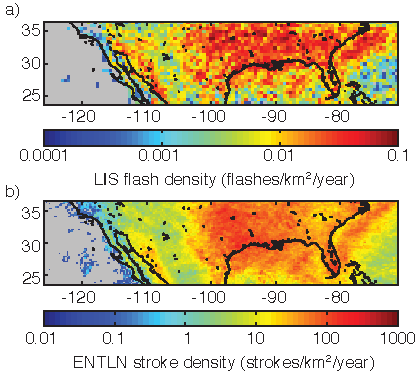
\includegraphics[width=19pc,angle=0]{entln_lis/Figures/density.pdf}
   \caption{a) LIS flash density at 0.5$^\circ$ grid spacing for fully viewed granules and
   		b) ENTLN stroke density at 0.25$^\circ$ grid spacing for 2011 -- May 2013.
   		Densities shown in counts/km$^2$/year; grid points with less than 30 counts are shown in gray.}
   \label{entln_lis:fig:density}
\end{figure}

Utilizing lightning networks requires a thorough understanding of what the networks detect and their limitations.
Examining detection efficiencies is one method to characterize the performance of networks, however such measures need to be used carefully as they often necessitate the assumption that the reference system is uniform, constant, and complete.
Using the LIS instrument allows for a robust and standard analysis of the ENTLN efficiency and accuracy.

\section{Performance}

\subsection{Matching}

ENTLN strokes are matched to LIS flashes when the ENTLN stroke is within a $\pm0.5^\circ$ box around the flash centroid and within $\pm10$~ms of the flash duration.
If multiple strokes are matched to a single LIS flash the timing and location of the stroke closest in time to the start of the flash is used as the best match; for the case of multiple flashes matched to a single stroke only the flash closest in time to the stroke is matched.
Matches between ENTLN-LIS had 30\% of LIS flashes matched to a single ENTLN stroke, with an overall mean multiplicity of 3.5.
Days with less than 30 total LIS flashes over North America are not used in this evaluation.

Evaluation of the effectiveness of LIS at observing ENTLN strokes utilizes the viewpoint granule data available with the flash level data.
The viewpoint granules give the start and end times of LIS observation for $0.5^\circ \times 0.5^\circ$ bins.
Full coverage for a given viewpoint granule is determined by the start and end times of the adjacent corner granules, as shown in Figure~\ref{entln_lis:fig:viewpoint}.
When LIS has at least partial coverage of the four corner viewpoint granules the center viewpoint granule is guaranteed to be in full view of the sensor.
The latest start time and earliest end time of the adjacent corner granules determines the time when the viewpoint granule is in full view of LIS.
Only ENTLN strokes and LIS flashes within viewpoint granules with full LIS coverage are used in this evaluation.
This restriction reduces the total number of LIS flashes by 30\% from $3.0 \times 10^5$ to $2.1 \times 10^5$ flashes; this ensures that all ENTLN strokes are within full view of LIS, removing edge and partial view cases.

\begin{figure}[ht!]
   \begin{center}
      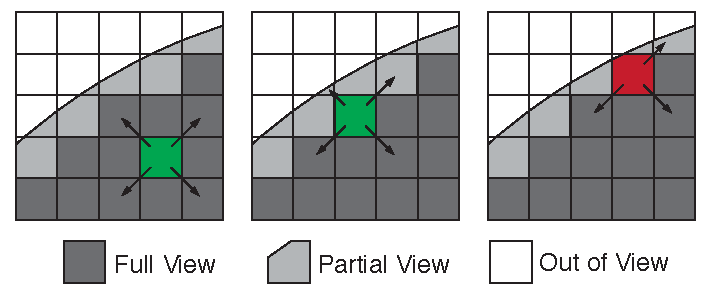
\includegraphics[scale=1]{entln_lis/Figures/viewpointGranule.pdf}
   \end{center}
   \caption{Classification of a viewpoint granule ($0.5^\circ \times 0.5^\circ$ bin) of LIS being in full view.
   If all four corner granules are at least partially viewed (left and center) the granule is in full view, if not it is only partially viewed (right).}
   \label{entln_lis:fig:viewpoint}
\end{figure}

An example of a single LIS overpass full coverage field of view, determined by the viewpoint granules, is shown in Figure~\ref{entln_lis:fig:overpass}.
This overpass occurred on 2012 April 21 from 15:20 -- 15:31 UTC.
Within the field of view LIS observed 220 flashes, of which ENTLN matched 66\%, shown in Figure~\ref{entln_lis:fig:overpass}a.
ENTLN strokes are considered within the field of view of LIS if they occur within the bounds of the viewpoint granule and between the start and end time of full LIS coverage.
In the pass shown in Figure~\ref{entln_lis:fig:overpass}b ENTLN detected 773 strokes, where 67\% were matched to LIS flashes.
In both cases the missed events are shown as red crosses.

\begin{figure}[t]
   \centering
   \noindent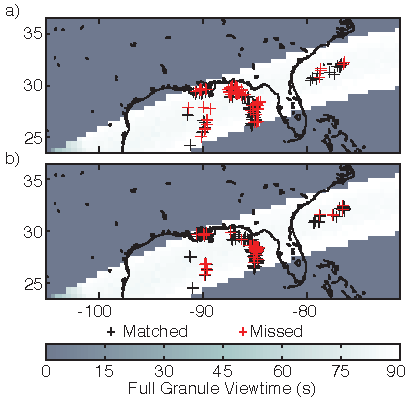
\includegraphics[width=19pc,angle=0]{entln_lis/Figures/overpass.pdf}
   \caption{LIS observation area for 2012 April 21 from 15:20 -- 15:31 UTC (day), seconds within full view of LIS shown in grayscale.
      		a) shows the LIS flashes matched by ENTLN (black crosses) during the overpass, red crosses are LIS flashes missed by ENTLN.
		b) shows the ENTLN strokes matched by LIS (black crosses) during the overpass, red crosses are ENTLN strokes missed by LIS.
		}
   \label{entln_lis:fig:overpass}
\end{figure}

\subsection{Accuracy}

System accuracy is measured by the timing and spatial offset between the lightning locations.
The timing offset ($t_{LIS} - t_{ENTLN}$), Figure~\ref{entln_lis:fig:accuracy}a, is sharply peaked at -1.9~ms, with ENTLN occurring before the LIS flash time; the median timing offset is 2.4~ms.
The LIS flash time is the time of the first LIS event in the flash group; 42\% of ENTLN strokes occurred 0 -- 4~ms before the start of the LIS flash, the remaining strokes correspond to subsequent discharges of the flash.

\begin{figure}[t]
   \centering
   \noindent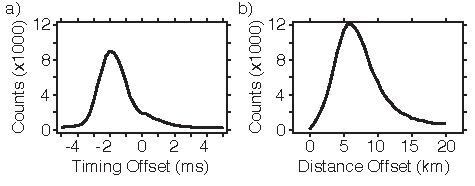
\includegraphics[width=19pc,angle=0]{entln_lis/Figures/accuracy.pdf}
   \caption{a) ENTLN-LIS timing offset ($t_{LIS} - t_{ENTLN}$) for the first matched stroke and
   		b) ENTLN stroke to LIS flash centroid distance for the first matched stroke.
   		Bin spacing set at (a) 0.25~ms and (b) 0.5~km.}
   \label{entln_lis:fig:accuracy}
\end{figure}

The median distance offset from the flash centroid is 7.0~km, as seen Figure~\ref{entln_lis:fig:accuracy}b, slightly above the LIS spatial resolution of 3 -- 6~km \citep{Christian1999}.
The location offset can be given in either kilometers from the flash centroid or in units of the estimated flash radius; the radius is calculated by considering the given LIS flash area as a circle.
Using the flash radius for distance results in a median offset of 0.80 flash radii; 65\% of the strokes are located within the visible extent of the flash.
A more refined location accuracy of ENTLN cannot be determined with LIS due to the spatial accuracy of the LIS pixels.

\subsection{Detection efficiency}

During the 2011 -- 2013 evaluation period the average daily detection efficiency of LIS flashes by ENTLN was 69\% $\pm$ 14\%.
The detection efficiency was marginally higher during the day at 72 $\pm$ 14\% and lower during the night at 65 $\pm$ 16\%.
The ENTLN decrease at night likely stems from the increased detection efficiency of LIS at observing lightning against a non-sunlit ground.
The spatial distribution of detection efficiency is shown in Figure~\ref{entln_lis:fig:map}a, with the daily variability shown in Figure~\ref{entln_lis:fig:de}a.
The spatially averaged detection efficiency is $61 \pm 16$\%, due to the uneven distribution of ENTLN stations with fewer stations in the West.
ENTLN detected 66\% of the $2.1\times10^5$ LIS flashes; within those flashes ENTLN detected $7.4\times10^5$ strokes ($<0.15$\% of total ENTLN strokes).
ENTLN has a spike of low detection efficiency in mid-June 2012 that is reflected in the LIS detection efficiency, this temporary decrease is likely due to a short-term issue with the network.

\begin{figure}[t]
   \centering
   \noindent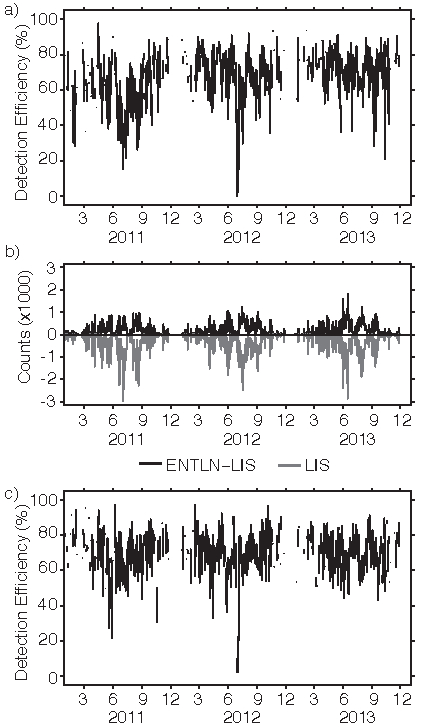
\includegraphics[width=19pc,angle=0]{entln_lis/Figures/de.pdf}
   \caption{a) ENTLN-LIS daily detection efficiency,
   		b) ENTLN-LIS total matches (black) and total LIS flashes (gray),
		c) LIS daily detection efficiency of ENTLN strokes.
		Gaps indicate days with less than 30 LIS flashes.
		}
   \label{entln_lis:fig:de}
\end{figure}

Within the LIS field of view ENTLN detected $7.1\times10^5$ strokes; of these strokes $4.8\times10^5$ were matched to LIS flashes for an overall LIS detection efficiency of ENTLN strokes of 68\%.
The spatial distribution of LIS detection efficiency of ENTLN strokes is shown in Figure~\ref{entln_lis:fig:map}b and the daily detection efficiency is shown in Figure~\ref{entln_lis:fig:de}c.
The average spatial detection efficiency of LIS is $67 \pm 13$\%, with an average daily detection efficiency of $70 \pm 12$\%.
Assuming the same multiplicity of 3.5 for the unmatched ENTLN strokes LIS missed $6.6\times10^4$, or 31\%, of all flashes.
To test for the possibility that the strokes not detected by LIS were improperly located, the waveforms for a random subset for ENTLN strokes were examined and the locations were found to be correct.

\begin{figure}[t]
   \centering
   \noindent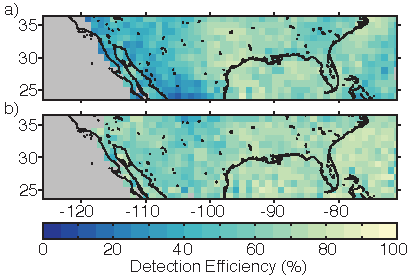
\includegraphics[width=19pc,angle=0]{entln_lis/Figures/map.pdf}
   \caption{a) Spatial distribution of ENTLN detection efficiency of LIS flashes and
   		b) LIS detection efficiency of ENTLN strokes.
   		Gray indicates $1^\circ \times 1^\circ$ bins with fewer than 30 LIS flashes.
		}
   \label{entln_lis:fig:map}
\end{figure}

Over land the highest ENTLN detection efficiency can be seen to occur in the Great Plains, Florida, and Texas.
There is decreased detection efficiency over both the Rocky and Appalachian Mountains, possibly caused by the lower sensor density in these regions.
While the mountain regions show lower detection efficiency with lower sensor density, there is a higher and more uniform detection efficiency within 450~km off the coasts.
The increased detection efficiency off of the coasts is a combined effect of fewer and stronger lightning strokes \citep{Hutchins2013, Rudlosky2010}.
LIS has a more uniform detection efficiency than ENTLN, as is expected from the imaging system.

On a daily scale the ENTLN-LIS detection efficiency, seen in Figure~\ref{entln_lis:fig:de}a, is fairly high through this time period, with brief periods of decreased performance.
The average daily detection efficiency is 69 $\pm$ 15\% with a $5^\text{th}$ to $95^\text{th}$ percentile range of 48\% -- 87\%.
Some of the larger decreases in detection efficiency match with the increased LIS flash counts in Figure~\ref{entln_lis:fig:de}b, such as early April 2012, late May 2012, and mid-July 2012.
On days with low LIS flash counts, $<40^\text{th}$ percentile, ENTLN detects $71\pm16$\% of flashes; while on days with high LIS flash counts, $>70^\text{th}$ percentile, ENTLN detects $65\pm10$\% of flashes.
During these times of increased lightning activity the ENTLN would need to raise the data compression threshold; causing it to miss weaker strokes that are still detected by LIS, resulting in the suppressed detection efficiency.

\subsection{Observation bias}

Two populations of ENTLN strokes are found with the comparison to LIS: the strokes matched to LIS flashes and the strokes that are unmatched.
Characteristics of these populations should show any bias of the flashes that are observed by LIS.
As ENTLN is a total lightning network it has the capability to detect and distinguish between CG and IC strokes.

To get a statistically robust measure of the percentage of cloud to ground strokes observed by LIS the matched LIS-ENTLN stroke data was randomly subdivided into 100 subsets of approximately $4.8\times10^3$ matched strokes.
Averaging these subsamples results in a statistically robust measure of the matched stroke CG percentage.
The populations of matched and unmatched LIS-ENTLN strokes are very similar; matched strokes are $20.3\pm0.6$\% CG and unmatched strokes are $21.8\pm0.8$\% CG.
The small difference between the populations shows that there is only marginal detection efficiency bias between lightning observed by LIS and ENTLN, with LIS slightly biased towards cloud flashes.

\section{Conclusion}

Characterizing the ENTLN, and other ground based networks, relative to a uniform detection system is critical in enabling the application of these networks in scientific and operational uses.
The Earth Networks Total Lightning Network was compared to the TRMM/LIS instrument on a stroke to flash matching level.
An average daily detection efficiency of $69\pm 14$\% was found for the continental United States for January 2012 -- May 2013 for $2.1 \times 10^5$ LIS flashes.
The relative location accuracy with respect to the flash centroid is 7.0~km and a timing offset to the start of the flash of 2.3~ms.
Within the LIS field of view ENTLN located $7.1\times 10^5$ strokes and $3.1\times10^8$ strokes within the entire evaluation region.
Of those located ENTLN strokes LIS had a $70 \pm 12$\% detection efficiency; leading to an estimated $6.6 \times 10^4$ flashes (31\% of total flashes) not detected by LIS.
Long range ground networks have the advantage of continuous real-time coverage of their encompassed region, resulting in more strokes detected along with capabilities such as stroke type discrimination and peak current estimation.

\subsection*{Acknowledgments for this Chapter}

The LIS flash data were obtained from NASA's Global Hydrology Resource Center (http://thunder.msfc.nasa.gov).


% ========== Chapter Land-Sea Contrast

\chapter{Land-Sea Contrast}
\label{thesis:chapter:landsea}

\section{Abstract}

A global contrast between oceanic and continental lightning very low frequency energy is observed using the World Wide Lightning Location Network (WWLLN).
Strokes over the ocean are found to be stronger on average than those over land with a sharp boundary along a majority of coastlines.
A linear regression method is developed to account for the spatial and temporal variation of WWLLN in order to perform a multi-year and global analysis of stroke energy distributions.

The results are corroborated with data from the Lightning Imaging Sensor, the Optical Transient Detector, and the Earth Networks Total Lightning Network.
These systematic comparisons lead to the conclusion that there exists a strong difference in the energetics between land and ocean thunderstorms that results in a higher fraction of more powerful strokes over the oceans. 


\section{Introduction}

Global surveys of lightning climatology have routinely shown more lightning activity over continents than over oceans \citep{Christian2003}.
The difference in activity is often attributed to changes in the convective regimes in the clouds.
\citet{Williams2002} and \citet{Williams2005} discuss aerosol concentration, wet bulb temperature, and cloud base height as dominant mechanisms of the difference in cloud electrification.
\citet{Zipser1994} suggests updraft velocity due to differential surface heating may lead to the difference in observed flash rates.
\citet{Boccippio2000} shows the total flash counts may be due to a lesser frequency of occurrence of oceanic storms and not a difference in the storms themselves.

Along with the difference in flash rates, there have been several observations suggesting an inherent difference in the lightning peak currents and optical radiance between land and ocean storms \citep{Seity2001, Ishii2010}. 
The U.S. National Lightning Detection Network (NLDN) observed higher average peak currents for negative cloud to ground (CG) strokes off of the coast, but the NLDN is limited in range for oceanic strokes near to coastlines \citep{Rudlosky2010, Lyons1998}.
\citet{Boccippio2000} observed with LIS/OTD an increase in the optical radiance and extent of oceanic flashes compared to those over land.
It was suggested that either a more energetic lightning generation process or a reduced cloud optical depth for the oceanic storms could produce the increased optical radiance.
However, it could not be be determined whether the more radiant flashes were caused by changes in the flashes or in the cloud optical depth using just the available satellite data.

As of January 2013, the World Wide Lightning Location Network (WWLLN, see wwlln.net) consists of 70 very low frequency (VLF) stations around the world allowing it to detect with a 5~km location and $15\mu$s timing accuracy and an estimated overall stroke detection efficiency of 11\% \citep{Hutchins2012a, Abarca2010,Rodger2009}.
An upgrade to the WWLLN allows for the network to measure radiated VLF stroke energies in addition to stroke locations \citep{Hutchins2012}.
The capability to measure stroke energies as well as the global coverage of the network allows for a global comparison of stroke energies over land and ocean regimes.

A comparison is made between the global stroke count climatologies of WWLLN and the 13-year Lightning Imaging Sensor (LIS) and 5-year Optical Transient Detector (OTD) flash count climatologies. 
The LIS (1997-present) and OTD (1995-2000) are nearly identical satellite-based lightning detectors flown in low earth orbit that observe total lightning activity from individual thunderstorms for 90 sec and 2 min, respectively, as the satellite passes overhead.
The LIS observes storms from an inclined orbit of 35$^\circ$ at an altitude of 402 km while the OTD observed storms from an inclined orbit of 70$^\circ$ at an altitude of 740 km \citep{Christian1999, Christian2003}.
Since WWLLN preferentially detects high-energy strokes \citep{Hutchins2012a} a direct comparison between the two systems, as described in \citet{Virts2013}, gives a comparison between high and low-energy strokes because of the detection biases of the two systems.

A second ground based detection network, the Earth Networks Total Lightning Network (ENTLN), is used to corroborate the results of the WWLLN data.
ENTLN is a higher density, broadband (1~Hz to 12~MHz receiver) network with about 500 operational stations in the United States \citep{Heckman2010}.
The network utilizes a time of arrival method to determine the location of each stroke, where a minimum of 8 stations is required to produce a valid solution.
From the recorded waveforms ENTLN infers polarity, peak current, and stroke type \citep{Liu2011a}.

\section{Linear Regression Analysis}
\label{secLinReg}

In order to compare WWLLN energy data over large spatial and temporal scales the data needs to be processed to account for the regional variations in detection efficiency and temporal changes in network performance.
To examine the spatial changes in stroke energy while accounting for network variability a linear regression method is developed.

Energy data for each day is binned every 0.5$^\circ$ in latitude and longitude.
The strokes in each bin are split into 10 energy deciles each containing $J$ strokes, with the mean energy of each decile, $i$, given by:

\begin{equation}
\overline{E_i} = \frac{\sum_{j=1}^J E_{i,j}}{J} 
\end{equation}

$\overline{E_i}$ has a power law dependence on decile number due to the lognormal distribution of stroke energies.
In order to make a linear regression between $\overline{E_i}$ and decile number $i$, the log$_{10}$ of $\overline{E_i}$ is used. 
A linear regression is found between $\text{log}_{10}(\bar{E_i})$ and $i$ to get an approximation of the mean energy with decile:

\begin{equation}
\text{log}_{10}(\overline{E(i)}) = C + \frac{\partial \text{log}_{10}(\overline{E_i})}{\partial i} i
\end{equation}

The first parameter from the fit, $C$, corresponds to the overall mean of the stroke energies in the particular spatial bin.
It is not used in this analysis since $C$ greatly depends on the network coverage at the time and location where it calculated.
$C$ will be larger where coverage is lower (WWLLN detecting only strong strokes) and lower with high coverage (WWLLN detecting both strong and weak strokes).
By using the regression method the network coverage and variable detection efficiency is factored out of the energy distribution into $C$ allowing for the shape of the energy distribution to be examined directly.

The second parameter, $\frac{\partial \text{log}_{10}(\overline{E_i})}{\partial i}$, is the slope of the regression and will be used to study the energy changes between land and ocean regimes.
$\frac{\partial \text{log}_{10}(\overline{E_i})}{\partial i}$ is the measure of how much (logarithmically) the average stroke energy changes from one decile to the next.
So a value of $\frac{\partial \text{log}_{10}(\overline{E_i})}{\partial i}$~=~0.1 at a location will increase the mean stroke energy by $10^{0.1}~=~25\%$ per decile, while a value of 0.2 will increase by $10^{0.2} = 58\%$ per decile.
The regression slope will be higher for either more high-energy strokes or fewer low-energy strokes.
The low-energy tail of the energy distribution is mostly set by the efficiency of the network, while the high end is always well detected even where the network is thin.
As $C$ captures the effects of the network performance, the slope of the regression will be mainly set by the energy of the strokes in the high-energy tail of the distribution.

An example of the linear regression method is shown in Figure~\ref{linRegTheory} using 15~days of data from 1-15 June 2012, separated into land (black) and ocean (gray) strokes.
The stroke counts are split into the ten decile bins outlined in Figure~\ref{linRegTheory}a.
$\overline{E_i}$ is shown in Figure~\ref{linRegTheory}b with the corresponding regressions plotted on top of the points.
Departures from the regression are acceptable as only the trend of increasing energy is important and not an exact fit.

\begin{figure}[ht!]
   \centering
   \noindent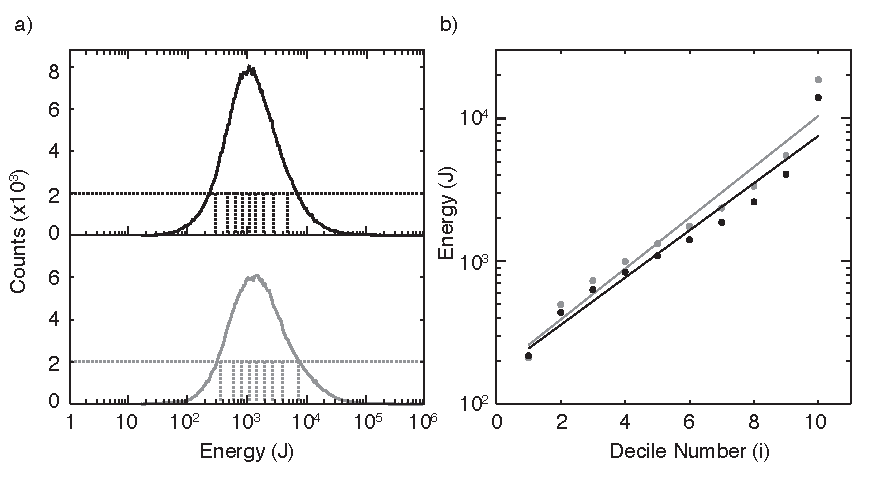
\includegraphics[width=20pc]{LandSea/Figures/1_linearRegression.pdf} 
   \caption{WWLLN data from 1-15 June 2012 for global strokes grouped into land (black) and ocean (gray) to demonstrate the linear regression method. a) Shows two energy distributions with the corresponding energy decile bins (dashed lines). b) is the plot of mean energy $\overline{E_i}$ in each bin with the linear regression (solid lines).}
   \label{linRegTheory}
\end{figure}

\section{Regression Slope Maps}

This technique is applied over 3 years of WWLLN data from May 2009 through May 2012 on a 0.5$^\circ$ grid, with the resulting regression slopes shown in Figure~\ref{regMap}.
For this analysis the calculated regressions must have an R-square value of at least 0.80 to be used.
In general higher slopes are seen over oceans and lower slopes over land, except for several regions of low detection efficiency (e.g. off the shore of Madagascar) and regions such as the Andes mountain range.
The map is similar to Figure~\ref{virts}, adapted from \citet{Virts2013}, which shows the ratio of the WWLLN normalized stroke climatology to the LIS/OTD normalized flash climatology.
The climatologies are normalized by their total stroke and flash counts respectively.
Figure~\ref{virts} is the spatial distribution of where WWLLN preferentially detects more strokes than LIS/OTD due to the bias of WWLLN towards detecting the most energetic strokes.
Comparing the stroke and flash data directly is possible as a majority of flashes have only the first, and strongest, stroke detected by WWLLN \citep{Abarca2010}.


\begin{figure}[ht!]
   \centering
   \noindent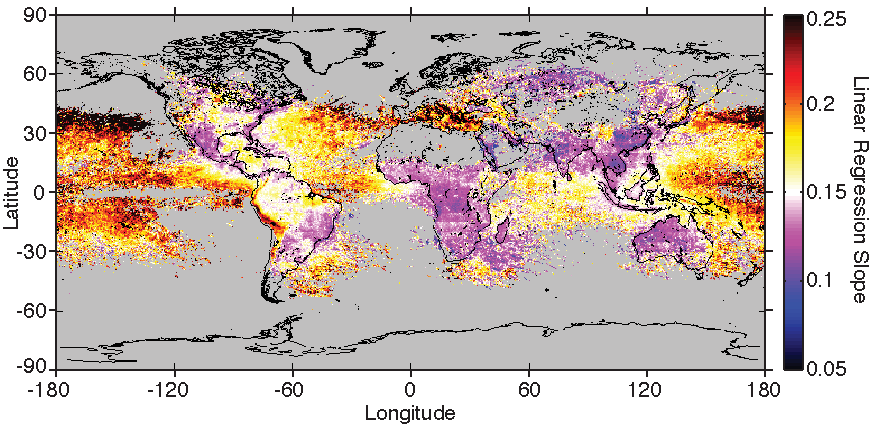
\includegraphics[width=20pc]{LandSea/Figures/2_regMap.pdf} 
   \caption{Slope of the linear regression used on the energy distribution as described in the text. High slope corresponds to a larger high-energy tail in the energy distribution as there are relatively more high-energy strokes.}
   \label{regMap}
\end{figure}

\begin{figure}[ht!]
   \centering
   \noindent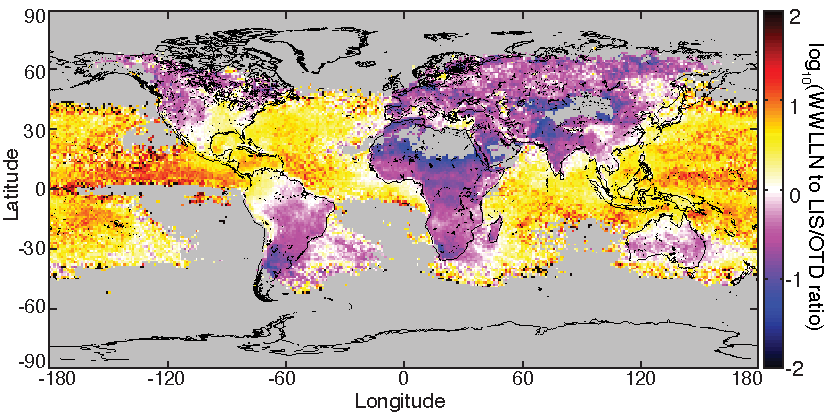
\includegraphics[width=20pc]{LandSea/Figures/3_lisMap.pdf} 
   \caption{Ratio of the WWLLN stroke count density climatology to the LIS/OTD flash count density climatology normalized by their relative total counts, adapted from \citet{Virts2013}.}
   \label{virts}
\end{figure}

The same linear regression was applied to the 2011 ENTLN data for a region over North America.
The absolute peak current was used for the regression instead of the stroke energy with the results in Figure~\ref{regMapENTLN}.
The land-ocean contrast is seen strongly in the ENTLN dataset, particularly over Mexico, Cuba and Haiti.
The difference also exists off the coast of the southeastern United States, but the contrast is not as strong (slope increase on the order of 0.01 instead of 0.1).

\begin{figure}[ht!]
   \centering
   \noindent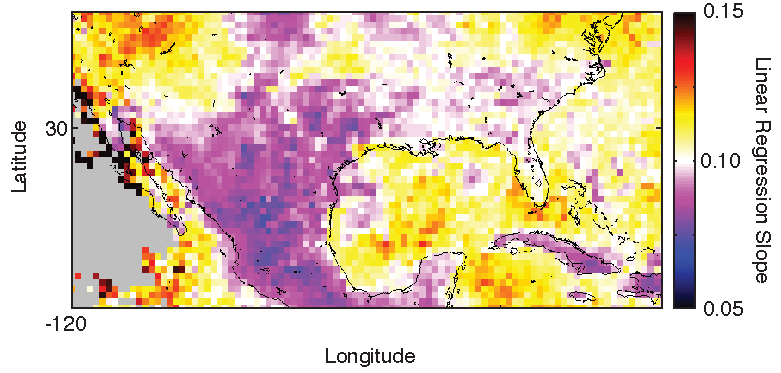
\includegraphics[width=20pc]{LandSea/Figures/4_regMapENTLN.pdf} 
   \caption{Slope of the linear regression used on the 2011 ENTLN absolute peak current distribution as described in the text. High slope corresponds to a larger high peak current tail in the distribution.}
   \label{regMapENTLN}
\end{figure}

For the ENTLN data the linear regression slopes only range from 0.05 to 0.15 compared to 0.05 to 0.25 for the WWLLN regressions.
Since energy is related to peak current by $E_{stroke} = 2229 \times | I_{peak} | ^{1.62}$ \citep{Hutchins2012}, $\text{log$_{10}$}(\overline{E_i})$ will be 1.62 times higher than $\text{log$_{10}$}(\overline{I_{peak,i}})$.
The range of the slopes for the ENTLN regression should then be correspondingly lower by a factor of 1.62, or from 0.03 to 0.15.

\section{Stroke Distributions}

The global ratio of the land and ocean stroke distributions clearly shows the prevalence of higher energy strokes over oceans.
The energy distribution of the WWLLN data is found for the set of strokes occurring over land and for the strokes occurring over oceans.
The ratio of these ocean and land energy distributions is shown in Figure~\ref{ratioComp}.

\begin{figure}[ht!]
   \centering
   \noindent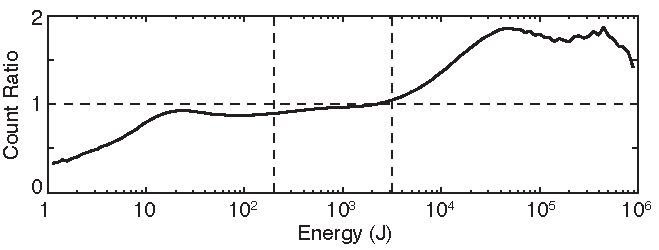
\includegraphics[width=20pc]{LandSea/Figures/5_distribution.pdf} 
   \caption{The ratio of ocean to land counts for WWLLN within each energy bin. The dashed horizontal line is a ratio of 1. The vertical dashed black lines in show the 15th and 85th percentile levels for the distribution.}
   \label{ratioComp}
\end{figure}

The ocean-land ratio starts increasing quickly with increasing energy at 3000~J, showing there are relatively more high-energy (top 15\% of stroke energy) strokes over the oceans than over land.
Similarly there is a general decrease in the ratio for decreasing strokes energies, with the downward trend interrupted with a small bump near 10~J.

\section{Regional Contrast}

In Figures~\ref{regMap} and~\ref{virts} there is an evident overall difference between land and ocean strokes, and it can be seen to vary sharply across most coastlines.
This raises the question of whether network detection efficiency across the coastline should be considered as a potential cause for the change.
Three regions are chosen for closer examination, shown outlined by the white boxes on top of a map of the WWLLN relative detection efficiency in Figure~\ref{wwlln_regional}a: North America, Western Africa, and Northeastern Brazil. 

\begin{figure}[ht!]
   \centering
   \noindent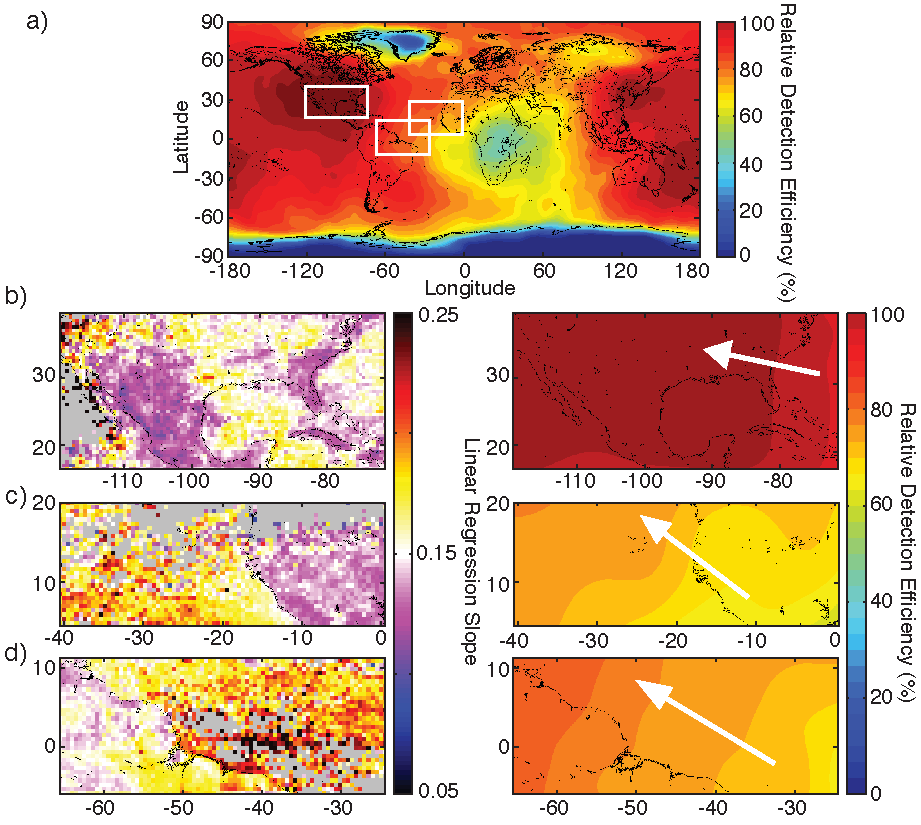
\includegraphics[width=20pc]{LandSea/Figures/6_wwlln_regional.pdf} 
   \caption{Regional maps of the linear regression slopes in the left column with respective WWLLN relative detection efficiency maps on the right. Selected regions outlined in a) on top of the map of the May 2009 through May 2012 average relative detection efficiency. b) shows the Continental United States and Gulf of Mexico, c) Western Africa, and d) Northeast Brazil. The white arrows point in the direction of increasing relative detection efficiency.}
   \label{wwlln_regional}
\end{figure}

WWLLN has an inherent bias towards more readily detecting low energy strokes over oceans than over land.
This is due to lower VLF wave attenuation over oceans, so low-energy strokes propagating over the ocean can reach more WWLLN stations compared to the same stroke traveling over land.
Hence WWLLN is naturally biased to predominately detect only the highest strokes over land, and relatively more lower energy strokes over water \citep{Hutchins2012}.
The method of linear regression described in Section~\ref{secLinReg} should remove most of this bias in WWLLN, and this can be checked in part by the recent work on relative detection efficiency \citep{Hutchins2012a}.
The three regions chosen in Figure~\ref{wwlln_regional} were chosen such that the gradient of relative detection efficiency is changing parallel to the coastline.

Over North America and the Gulf of Mexico, Figure~\ref{wwlln_regional}b, the strokes over Mexico, Florida, Cuba, and Haiti are all weaker than those over the nearby ocean.
This is also seen with the ENTLN in Figure~\ref{regMapENTLN}.
The relative detection efficiency (see \citet{Hutchins2012a}) is fairly uniform over this region with the largest change occurring over the Atlantic where there is no change to the regression slope.
Over the central United States there is a large region of high stroke energies, this is also observed in the ENTLN regression slope (Figure~\ref{regMapENTLN}) and LIS/OTD count ratio (Figure~\ref{virts}) data. 

In Western Africa, Figure~\ref{wwlln_regional}c, there is a clear difference between the land and the ocean.
The coast shows a very sharp change in the stroke strength.
The changing detection efficiency in this case is parallel to the coast and would not affect the variation in stroke energy at the coastline.

The difference in Brazil, shown in Figure~\ref{wwlln_regional}d, is similar to that over Western Africa with the exception of the increased stroke energies seen over Amazon River delta.
Even with the increase over the delta there is still a contrast off of the coast with the change in regression slope comparable to the coastline northwest of the delta.

\section{Conclusion}

A linear regression method is developed and applied to the WWLLN dataset in order to examine global and regional changes of lightning stroke strength over several years of network data.
Through comparing WWLLN, ENTLN, and LIS/OTD the difference between stroke strength is seen to be highly dependent on whether the storms occur over land or over ocean with a sharp boundary occurring along most coastlines.
Smaller regions are examined to show that the contrast along coastlines is not due to abrupt changes in the detection efficiency of the networks.
The sharpness of the coastal changes, less than 100~km, suggests the effect is due to a local phenomena and not be caused by large scale changes in the convective land-ocean regions.
Changes exist within continental regions, but these transition were not examined as the underlying change between regimes is not as sharp as for coastlines.




% ========== Chapter VLF Propagation

\chapter{VLF Propagation}
\label{thesis:chapter:prop}

\section{Overview}

The World Wide Lightning Location Network (WWLLN) is used to measure the normalized lightning electric field at three network stations in order to examine the sferic attenuation between the stroke and the station.
The electric field measurements are normalized to the square root radiated very low frequency (VLF) stroke energy to allow direct comparisons of the many stroke-station paths seen by WWLLN.
WWLLN observes a strong dependence of VLF propagation on magnetic azimuth similar to past work.
From WWLLN the average attenuation over the water of eastward-propagating sferics is found to be $1.13 \pm 0.35$~dB/Mm during the day and $0.71 \pm 0.68$~dB/Mm at night, with westward-propagating sferics having average attenuation rates of $2.98 \pm 0.68$~dB/Mm and $2.66 \pm 0.39$~dB/Mm for day and night respectively.

The propagation dependence on magnetic azimuth stems from the polarization of the VLF wave with respect to the electron motion in the ionosphere .
Ionospheric electrons are constrained to gyrate in one direction; for VLF waves propagating eastward the polarization of the wave is in the same direction as the electrons providing more efficient propagation, the opposite in the case for westward propagating waves.
There is then no change in propagation for waves aligned with the magnetic field, e.g. northward or southward propagating waves.

Past experimental work has shown a strong dependence of VLF attenuation on the magnetic azimuthal angle of propagation.
\citet{Wait1960a} provide an in-depth analysis of the theoretical background.present a theoretical background for why the attenuation changes with azimuth.
By measuring the signal strength from the same nearly antipodal transmitter along the short and long great circle path, \citet{Crombie1958} found less attenuation for the eastward propagating signals.
Similarly \citet{Taylor1960a} showed that eastward propagating VLF waves have 1 -- 3 dB/Mm less attenuation than westward propagating waves.
Recently \citet{Jacobson2012} used negative cloud-to-ground strokes to examine ionospheric reflectance and also found a strong azimuthal dependence to the measurements.

The past work has examined stationary VLF transmitters with either a few receivers or one moving receiver.
Recent work by \citet{Burkholder2013} utilized the World Wide Lightning Location Network (WWLLN) to examine how eastward and westward propagating VLF sferics couple into the ionosphere.
This work motivated us to use the many stroke-receiver paths of WWLLN to study the azimuthal dependence of VLF propagation within the Earth-ionosphere waveguide.

The global coverage of the network allows for many long range stroke-receiver paths with which to estimate VLF attenuation rates.
The sferic attenuation for a single station can be found with WWLLN by comparing the stroke energies measured by the network to the RMS electric field measured at a single WWLLN station.
Using WWLLN allows for the azimuthal propagation effects to be examined at all magnetic azimuths for both all-night and all-day paths.
The measured electric fields and observed attenuation rates can be directly compared to the theoretical predictions of \citet{Wait1960a} and \citet{Taylor1960a}.
%% Page 209-210
By examining the propagation it is shown that WWLLN captures the effects of propagation and that the theories are applicable for non-stationary transient sources.

\section{Path Selection}

To examine eastward and westward propagation three WWLLN stations were chosen based on their island locations: Suva, Tahiti, and Honolulu.
These stations were selected as a majority of their stroke-receiver paths are over water, so the effects of variable ground conductivity can be ignored. 

The WWLLN energy calculation uses the LWPC code that accounts for eastward and westward propagation.
However each WWLLN energy measurement is the median energy of several WWLLN stations, so by selecting strokes with a similar number of stations to the east and west the azimuthal dependence computed by LWPC can be minimized.
There is allowed to be at most 25\% more WWLLN stations to the east or west of a located stroke, where this abundance is defined by: $|n_{east} - n_{west}| / n$.
For example, a located stroke with 1 station to the north, 2 east, and 3 west will have a westward abundance of 16.7\% and would be included in the analysis.

With these three stations the WWLLN data are reduced to only consider sferics that crossed at most 5\% land, and propagated in either at least 95\% day or night ionospheric conditions.
The stroke energy uncertainty (median absolute deviation of contributing stations, see \citet{Hutchins2012}) is limited to a maximum of 10\%.
Further the data are reduced by selecting only strokes with a similar number of locating WWLLN stations situated to the east and west as described above.
These requirements reduce the stroke-receiver paths in the WWLLN dataset to 0.2\% of the total paths for each station; where 87\% occur during the day and 13\% occur at night.
This resulted in over $2\times10^6$ total stroke-receiver paths used in this Chapter.

The subset of data contains the RMS electric field at each station, the distance to the strokes, and the VLF energy of the stroke.
VLF stroke energies and station measured electric fields both vary over several orders of magnitude.
All station electric fields (in units of $1 \mu V m^{-1}$) are normalized by the square root of the stroke energy (in $J$) to allow for direct comparisons between differing source energies.
The stroke energy normalization gives the electric field in dB above $1 \mu Vm^{-1}/J^{1/2}$.
Changes in the normalized electric field with stroke distance gives the attenuation of the lightning sferic for that distance interval, reported as the dB/Mm decrease. 

Normalized field values are grouped into 45$^\circ$ azimuth and 500~km distance bins.
An example of all of the distance bins for a given azimuth for one station is shown in Figure~\ref{azimuth:fig:azimuthCalculation} (northwestward-propagation during the day for Honolulu station).
Each distance bin has a distribution of normalized field values with the spread a result of differing ionospheric conditions, uncertainty in the energy measurements, and changes in ground conditions at the station.
Because of this spread the median value of the normalized field is used for each distance-angle combination (shown as the solid black line).
At least 15 strokes are required for each distance bin at a given azimuth in order to calculate a reasonable median.
The magnetic azimuth used is the average magnetic azimuth over the path of wave propagation.

 \begin{figure}[h!t]
   \centering
   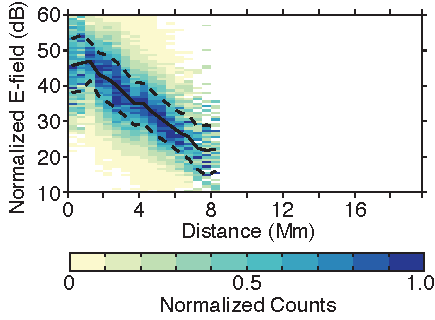
\includegraphics[scale=1]{Azimuth/Figures/azimuthCalculation.pdf} 
   \caption{Normalized electric field values for the 315$^\circ$ azimuth bin for the Honolulu station during the day.
   	Counts are normalized to the maximum value in each distance bin.
	The median (solid) and median absolute deviation (dashed) values are plotted on top of the distribution.
	Distances with less than 15 total strokes are not plotted or used.}
   \label{azimuth:fig:azimuthCalculation}
\end{figure}

\section{Azimuthal Dependence}

For the three stations data were used from May 2009 to May 2013, resulting in $2.1\times10^6$ stroke-station paths to analyze.
The results are split into the 8 azimuth octants for day paths and night paths as shown in Figure~\ref{azimuth:fig:azimuth}.
For the three stations the westward propagating waves (green) show higher attenuation (electric field change per unit distance) than for the eastward propagating waves (red).
The attenuation is also seen in the maximum distance that strokes are detected, with night (eastward) paths detectable at farther distances than day (westward) paths.

 \begin{figure}[h!t]
   \centering
   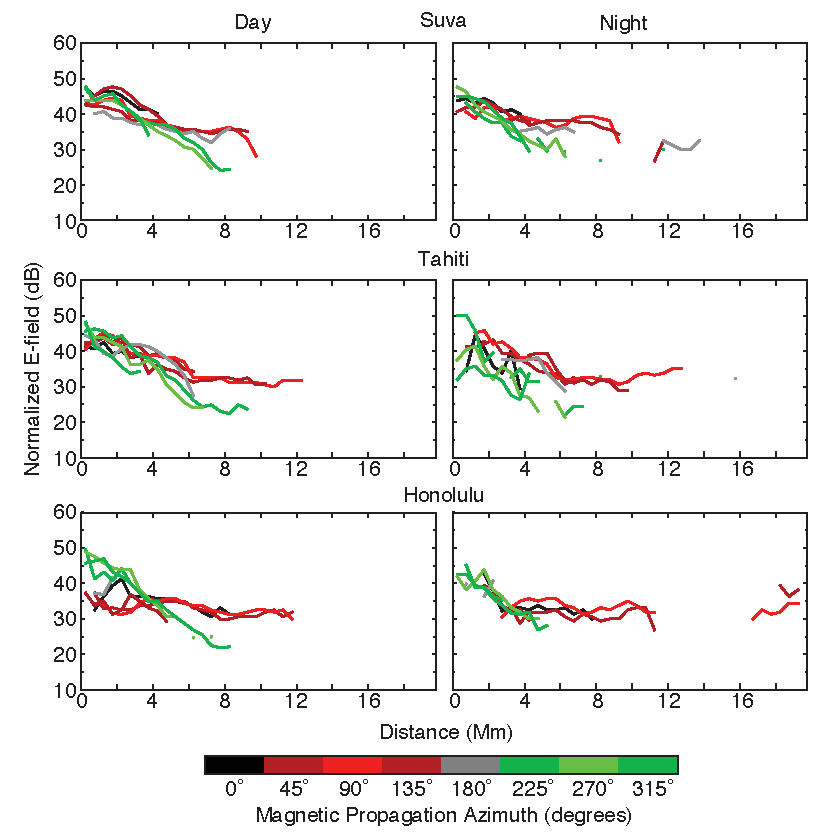
\includegraphics[scale=1]{Azimuth/Figures/e-field_3.pdf} 
   \caption{Station RMS electric field vs distance for Suva, Tahiti, and Honolulu.
   	Electric field is normalized by the square root stroke energy and given in dB above $1 \mu Vm^{-1}/J^{1/2}$.
	Day ionosphere paths are in the left column and night ionosphere paths in the right column.}
   \label{azimuth:fig:azimuth}
\end{figure}

For some stations, such as Honolulu in Figure~\ref{azimuth:fig:azimuth}, the difference between eastward and westward sferics is quite clear during the day at all distance ranges, and between day and night.
For other stations, such as Suva, the difference in propagation direction is not distinct for all azimuths.
Suva and Tahiti stations do not show a differentiation in attenuation until the waves have propagated some distance from the stroke, for example the night strokes for Suva in Figure~\ref{azimuth:fig:azimuth} are indistinguishable until 4~Mm.

In all cases the slopes of the field strength curves in Figure~\ref{azimuth:fig:azimuth} show that the eastward sferics exhibit less attenuation than westward sferics away from the stroke.
In cases like Honolulu the westward sferics initially have a lower normalized electric field, but the attenuation rate of these sferics is still lower than the eastward sferics.
  
The overall behavior of the VLF waves observed by WWLLN can be seen in the combined station data.
The station-stroke pairs were combined for all stations to give a single dataset of paths, shown in Figure~\ref{azimuth:fig:azimuthAverage}.
The westward sferics in both day and night have similar electric field to the eastward sferics with the distinction developing at greater than 4~Mm from the stroke.
There is a small upturn in field strength as the sferics propagate past 10~Mm because the waves are re-focusing when they cross the halfway point to their antipode.

\begin{figure}[h!t]
    \centering
    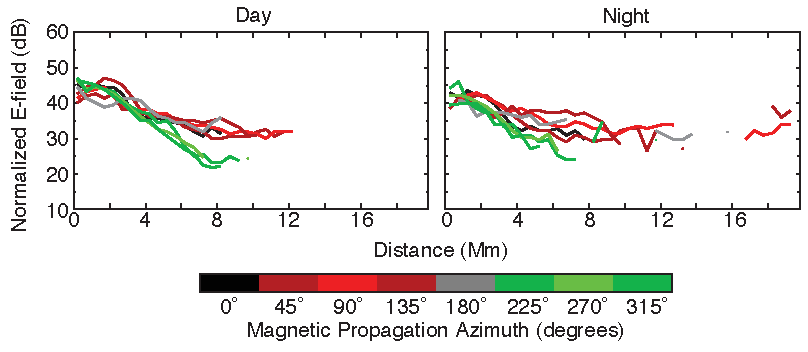
\includegraphics[scale=1]{Azimuth/Figures/azimuthAverage.pdf} 
    \caption{Combined station normalized electric field for the three selected stations.
    	Shown in dB above $1 \mu Vm^{-1}/J^{1/2}$.}
    \label{azimuth:fig:azimuthAverage}
 \end{figure}

The method for estimating the attenuation and the uncertainty is outlined in Figure~\ref{azimuth:fig:attenuationCalculation} using the station averaged eastward-propagating electric field values as an example (red line in Figure~\ref{azimuth:fig:azimuthAverage}).
The following fitting and smoothing method is used to estimate the attenuation to remove the noise in the direct attenuation (Figure~\ref{azimuth:fig:attenuationCalculation}b). 
First, the normalized electric field versus distance curves are smoothed and fitted to quadratics for the bins that have data, as shown with the dashed line in Figure~\ref{azimuth:fig:attenuationCalculation}a.
Second, the attenuation between each bin of the fit (the slope of Figure~\ref{azimuth:fig:attenuationCalculation}a) is found and shown in Figure~\ref{azimuth:fig:attenuationCalculation}b.
Lastly, the attenuation for a given electric field curve is calculated by the mean of the fitted attenuation where positive attenuation corresponds to a signal loss over distance.
The standard deviation of the attenuation is taken as the uncertainty in the attenuation measurement.
In the example of Figure~\ref{azimuth:fig:attenuationCalculation} the fitted attenuation is $1.13 \pm 0.35$~dB/Mm whereas the attenuation directly from the data (solid line in Figure~\ref{azimuth:fig:attenuationCalculation}b) is $0.79 \pm 2.34$~dB/Mm.
The increased uncertainty in the direct attenuation is due to the variations in attenuation between successive 500~km distance bins.
The fitted attenuation is used for all of the following attenuation values.

There is an inherent geometric factor to the measured attenuation values.
As the wave expands radially out from the lightning source it is moving through the spherical waveguide of the Earth and Ionosphere.
This expansion adds in a factor of $\frac{1}{sin(d/R)}$ to the received wave power at a station, or $\frac{1}{sin(d/R)^{1/2}}$ to the measured electric field.
In the geometric factor $d$ is the great circle distance from the wavefront to the lightning source and $R$ is the radius of the Earth.
Because past models, such as \citet{Wait1960a}, include the effects of the geometric factor in their predictions and past measurements do not correct for it, the measured attenuations will not be corrected for the geometric effect.

\begin{figure}[h!t]
    \centering
    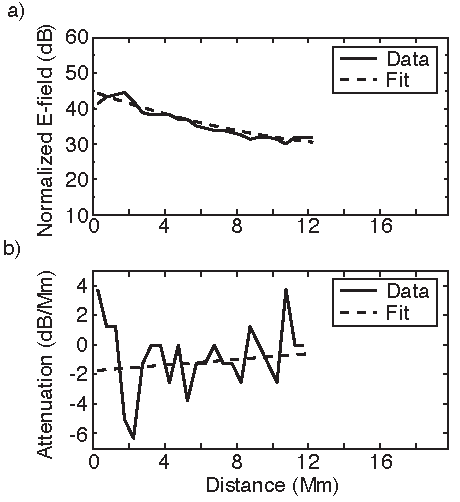
\includegraphics[scale=1]{Azimuth/Figures/attenuationCalculation.pdf} 
    \caption{Method for calculating the attenuation.
    	In a) the normalized electric field vs distance data (solid line) and the fitted quadratic (dashed line).
	In b) the change in electric field with distance step (derivative) for the data (solid line) and the fit (dashed line) normalized to dB/Mm.}
    \label{azimuth:fig:attenuationCalculation}
 \end{figure}

Overall there is an average attenuation of $1.87 \pm 1.06$~dB/Mm for all azimuths and times.
Within the first 4~Mm of the stroke the attenuation is fairly high for both day and night, with $2.08 \pm 0.90$~dB/Mm during the day and $2.09 \pm 1.02$~dB/Mm at night.
Beyond 4~Mm the attenuation decreases to $1.29 \pm 1.09$~dB/Mm for day and $0.24 \pm 0.48$~dB/Mm for night.
The 4~Mm cutoff was chosen based on Figure~\ref{azimuth:fig:azimuth} and~\ref{azimuth:fig:azimuthAverage} where the eastward and westward-propagating sferics start to clearly differentiate.
The increased attenuation near the stroke is likely due to the fast decay of higher order modes that cannot propagate far from their source \citep{Wait1970}.

For eastward sferics the average attenuation is $1.13 \pm 0.35$~dB/Mm and $0.71 \pm 0.68$~dB/Mm for day and night; for westward sferics attenuation is higher with rates of $2.98 \pm 0.68$~dB/Mm and $2.66 \pm 0.39$~dB/Mm for day and night paths.
The difference in attenuation between eastward and westward-propagating sferics is an increase of  1.9~dB/Mm for day and 2.0~dB/Mm for night.
  
\section{Comparisons to Theory}

The azimuthal variability of the WWLLN normalized electric-field attenuation is directly compared to the azimuthal variance predicted by \citet{Wait1960a} in Figure~\ref{azimuth:fig:attenuationTheory}.
The azimuthal variation, P$(\phi)$, is found by comparing the attenuation with the presence of a magnetic field to the attenuation without.
For the WWLLN data the average attenuation of all azimuths is taken as representative of the attenuation with no magnetic field.
The variability of the attenuation rate (in dB/Mm) with magnetic azimuth from \citet{Wait1960a} is approximated as $P(\phi) = - 0.3 \times \text{sin}(\phi) + 1$.

\begin{figure}[h!t]
   \centering
   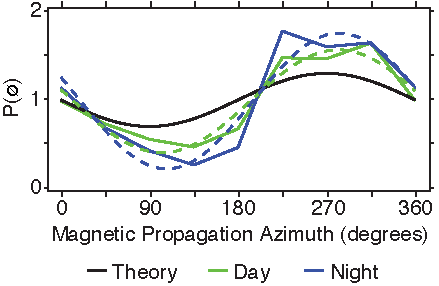
\includegraphics[scale=1]{Azimuth/Figures/attenuationTheory.pdf} 
   \caption{Dependence of attenuation with magnetic azimuth shown as P($\phi$), the attenuation normalized to attenuation with no magnetic field.
   	Shown for \citet{Wait1960a} (black), day paths (green), and night paths (blue).
	The best fit curves are shown as dashed lines.
	Day and night paths are normalized by their mean.}
   \label{azimuth:fig:attenuationTheory}
\end{figure}

The average attenuation azimuthal variation was fit to the same form as the theory ($P(\phi) = - a~\times~\text{sin}(\phi + b) + 1$) with the resulting fits shown in Figure~\ref{azimuth:fig:attenuationTheory}.
The leading coefficient, $a$, gives the relative variation in attenuation with azimuth; how much attenuation rates will change between northward/southward and eastward/westward propagating sferics.
The day attenuation best fit is $P(\phi) = - 0.58 \times \text{sin}(\phi + 348^\circ) + 1$ and the night attenuation best fit is $P(\phi) = - 0.76 \times \text{sin}(\phi - 344^\circ) + 1$.
Both day and night paths show twice the amplitude relative to the theory ($a_{theory} = 0.3$), with a weaker day dependence and a stronger night dependence, $a=0.58 \pm 0.18$ and $a=0.76 \pm 0.26$ respectively.
On average the day measurements vary from the theory by 19\% and the night measurements by 34\%.

In previous measurements of 3 -- 30~kHz VLF attenuation \citet{Taylor1960a} observed westward VLF paths to exhibit 1-3~dB/Mm more attenuation than eastward paths.
This is in line with the WWLLN measured increase of 1.9-- 2.0~dB/Mm from eastward to westward-propagating sferics.
Similarly the LWPC model shows an attenuation increase of 2~dB/Mm from eastward to westward-propagating sferics for equatorial day paths over the Pacific Ocean.
The model also gives a 28\% to 37\% variability of attenuation between propagation directions, relative to northward propagation, compared to 30\% for \citet{Wait1960a} and 58\% to 77\% for WWLLN.

The measured attenuation rates of WWLLN are within the previously measured ranges of attenuation and within the same difference between propagation directions.
However, the total azimuthal dependence of VLF propagation has been observed to be greater than that of the theoretical model of \citet{Wait1960a} and the propagation model LWPC.
The inconsistency may stem from the WWLLN measurements being the average over a range of frequencies while past measurements and models are for specific narrow frequencies, usually VLF transmitters.

\section{Conclusion}

Four years of WWLLN data were used to analyze the normalized VLF electric field from lightning at three island stations, with the variation with magnetic azimuth compared to theoretical results.
The electric fields were used to calculate the average attenuation in the 8 -- 18~kHz band at different propagation azimuths.
The stroke-receiver paths were selected for sferics propagating over at least 95\% water and under either 90\% day or 90\% night ionospheric conditions.

It was found that compared to day propagation, night propagating sferics have higher attenuation close to the stroke ($2.09 \pm 1.02$) with less attenuation farther out ($0.24 \pm 0.48$).
Similarly attenuation of night sferics have a higher dependence on magnetic azimuth compared to day sferics.
Variations with magnetic azimuth showed that westward propagation had 1.9 -- 2.0~dB/Mm more attenuation than eastward propagation for both day and night ionospheric conditions.

Combining three optimally placed WWLLN stations allowed for this examination of the azimuthal dependence of VLF attenuation.
Utilizing more of the 70 stations will allow for further investigation of VLF attenuation rates with other path parameters such as ocean salinity, ice, and ground conductivity.



% ========== Chapter Global Electric Circuit

\chapter{Global Electric Circuit}
\label{thesis:chapter:gec}

\section{Overview}

The diurnal variation of the global electric circuit is investigated using the World Wide Lightning Location Network (WWLLN), which has been shown to identify nearly all thunderstorms (\citet{Jacobson2006c}, using WWLLN data from 2005).
To create an estimate of global electric circuit activity a clustering algorithm is applied to the WWLLN dataset to identify global thunderstorms from 2010 -- 2013.
Annual, seasonal, and regional thunderstorm activity is investigated in this new WWLLN thunderstorm dataset in order to estimate the source behavior of the global electric circuit.
Through the clustering algorithm, the total number of active thunderstorms are counted every 30 minutes creating a measure of the global electric circuit source function.
The thunderstorm clusters are compared to precipitation radar data from the Tropical Rainfall Measurement Mission satellite and with case studies of thunderstorm evolution.

The clustering algorithm reveals an average of $660 \pm 70$ thunderstorms active at any given time with a peak-to-peak variation of 36\%.
The highest number of thunderstorms occurs in November ($720 \pm 90$) and the lowest number occurs in January ($610 \pm 80$).
Thunderstorm cluster and electrified storm cloud activity are combined with thunderstorm overflight current measurements to estimate the global electric circuit thunderstorm current contribution to be $1090 \pm 70$~A with a variation of 24\%.
By utilizing the global coverage and high time resolution of WWLLN, the total active thunderstorm count and current is shown to be less than previous estimates based on compiled climatologies.

Diurnal variation in global thunderstorm activity was original observed by \citet{Wilson1921} and \citet{Whipple1929} through a combination of thunderstorm day and electric field measurements.
Strong correlations between thunderstorm activity and fair weather return current led to the model of the global electric circuit, a system of ionospheric charging and discharging through thunderstorms and fair weather return currents.
Studies to date have estimated that globally there are 1000 -- 2000 thunderstorms active at any one time; most concentrated over tropical landmasses, covering 1 -- 10\% of Earth's surface \citep{Markson1978, Rycroft2011a, Singh2011a}.
Previous work on diagnosing the generator source of the global electric circuit used several methods:  long time scales \citep{Tinsley2007, Liu2010}, mathematical models \citep{Kasemir1977, Hays1979, Roble1991}, engineering models \citep{Ogawa1985, Kartalev2004, Rycroft2006}, parameterization \citep{Price1992, Williams1985}, and thunderstorm overflight estimates \citep{Mach2011}.
Most work with the global electric circuit uses long term averaging to recreate the known Carnegie curve of \citet{Whipple1929}, yet short time scales do not match the long term averaging \citep{Holzworth1984a}.
The variation of the global electric circuit changes on short time scales that is not resolved in past models or with long term averaged observations.
The global electric circuit is an important component to the solar-terrestrial system creating a link between solar activity, the ionosphere, aerosols, cloud microphysics, thunderstorms, weather, and climate \citep{Tinsley2007, Holzworth1986}.

Individual lightning strokes and flashes are not yet a reliable method of characterizing the source of the global electric circuit, but global thunderstorm activity is a reliable measure.
\citet{Ruhnke1969} proposes that the conduction and displacement currents above thunderstorms are the global electric circuit generators source as they vary slowly through the evolution of a thunderstorm and the currents are fairly independent from impulsive events like lightning.
\citet{Krider1985} looked at displacement currents below a thunderstorm to find them steady with abrupt, but insignificant, changes due to lightning.
\citet{Rycroft2000c} created an engineering model with three different regions for the the return current, concluding that sprites, lightning, and other transients will have little direct effect on the global electric circuit.
\citet{Stergis1957} showed that cloud to ground lightning is not necessary for upward current from thunderstorms.
With a numerical model of a dipolar thunderstorm \citet{Tzur1985} estimated the average upward current contribution of a thunderstorm to the global electric circuit to be 0.7~A per thunderstorm.
Similarly, with a combination of numerical and analytical models of dipolar thunderstorm, \citet{Driscoll1992} estimated a total contribution of 0.4~A to the global circuit per thunderstorm.
Unlike the other models, \citet{Mareev2008} estimated a 50 -- 400~A current contribution directly from global lightning;  with a similar model \citet{Mallios2012} investigated the efficiency of lightning and found lightning only contributed 1\% (3~A) of the total 300~A contribution from thunderstorms.
These models show that thunderstorms contribute an appreciable upward current to the global electric circuit with a wide range of estimated current contributions.

Balloon and aircraft overflights have been used to estimate the total current contributions from thunderstorms to the global electric circuit.
\citet{Stergis1957} found thunderstorm currents ranging from 0.6 -- 4.3 A, with an average of 1.3 A; these estimates are the lower bound with uncertainties of up to 50\%.
\citet{Blakeslee1989} shows the upward current generated by a thunderstorm to range between 0.1 -- 6~A with an average current between 0.5 -- 1~A.
Other studies show current density over thunderstorms ranging from 10 -- 40 pA/m$^2$ \citep{Holzworth1981} to $-20$ -- 33~nA/m$^2$ \citep{Mach2009}.
The overflights in previous research found no consistent parameterization between lightning rates and fair weather return current, but recent balloon work found strong correlation between global lightning activity and the fair weather return current on short time scales \citep{Holzworth2005}.
Lightning stroke activity and locations cannot directly provide estimates of the global circuit, however they can be used for directly locating and defining active thunderstorm areas and relative intensities.

Compared to satellite and balloon observations, ground based lightning networks have the advantage of continuous observation of large regions.
Global very low frequency networks, such as the World Wide Lightning Location Network (WWLLN), are capable of locating lightning around the entire globe.
\citet{Holzworth2005} compared the stroke counts of a nascent WWLLN to the fair weather return current and found strong temporal correlation between the measurements.
A better measure of global circuit activity is the total number of active thunderstorms around the globe; applying clustering algorithms to lightning network data enables the network to locate, track, and monitor global thunderstorm activity.

The WWLLN data are clustered into thunderstorms with the Density-Based Spatial Clustering of Application with Noise (DBSCAN) algorithm \citep{Ester1996, Kriegel2011a}.
DBSCAN was chosen as the clustering algorithm for several key features: the capability to handle noise, no requirement to specify the number of clusters, arbitrary cluster shapes, and the insensitivity to the ordering of the data.
Clustering lightning strokes into thunderstorms cannot require a designated number of clusters before clustering, as the total number of thunderstorms is not known before clustering.
Similar algorithms, such as Ward's Method, cluster into large unphysical thunderstorms due to noise \citep{Ward1963}.
In another approach \citet{Mezuman2013a} used a connected components methods to cluster the WWLLN data.
They found global thunderstorm activity to average near 1000 thunderstorms with significant daily variability.
The resulting WWLLN lightning clusters are representative of the lightning active stage of the thunderstorm.
Even though the electrically active portion of a thunderstorm extends beyond the active lightning stage \citep{Jacobson1976, Stolzenburg2010}, the clustered lightning active stage in this work will be referred to as the clustered thunderstorm or thunderstorm clusters.

\section{Clustering}

\subsection{DBSCAN}

DBSCAN clusters n-dimensional points based on the distance between the points, a length scale $\epsilon$, and the minimum number of points necessary to form a cluster, $minPts$ \citep{Kriegel2011a}.
Points in a cluster are either core points or non-core points; a point is a core point of a cluster if there are $minPts - 1$ other points within $\epsilon$ distance of that point (resulting in $minPts$ points within distance $\epsilon$).
In Figure~\ref{gec:fig:dbscan} the distance $\epsilon$ is represented by the circle around each point, lines connect points within $\epsilon$ of each other, and core points are shown as filled symbols.
Points that are within $\epsilon$ of one core point, but less than two core points ($minPts$ = 3), are added to the cluster as non-core points and cannot be used to add more points into the cluster.
For example the unfilled triangle symbol in Group~1 of Figure~\ref{gec:fig:dbscan} is within $\epsilon$ of one core point and clustered into the group as a non-core point, but cannot connect further unclustered points (crosses) into the cluster.

 \begin{figure}[ht!]
    \centering
    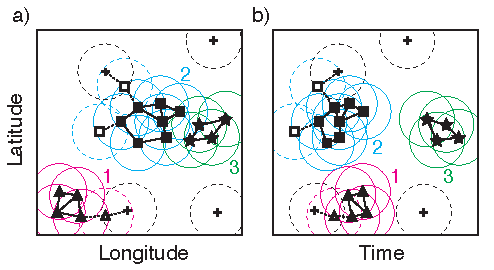
\includegraphics[scale=1]{GEC/Figures/dbscan.pdf}
    \caption{DBSCAN clustering example, with $minPts = 3$, showing the same clusters located in a) latitude and longitude and b) latitude and time.
    		 Solid rings show the $\epsilon$ distance from core points (filled), dashed rings are for non-core points (unfilled).
		 Triangles (1), squares (2), and stars (3) show clustered points, crosses are non-clustered points.}
    \label{gec:fig:dbscan}
 \end{figure}

WWLLN lightning strokes are separated by three dimensions: latitude, longitude, and time.
With time as a consideration two clusters that appear to overlap in Figure~\ref{gec:fig:dbscan}a, group~2 (blue) and group~3 (green), are separated by $\epsilon$ in time and are distinct groups as seen in Figure~\ref{gec:fig:dbscan}b.
DBSCAN is a physically realistic algorithm for clustering lightning data, such as WWLLN data, as the core points of a thunderstorm are the intense lightning centers while edge points are clustered but do not connect disparate lightning centers.

\subsection{Clustering WWLLN}

Accurate thunderstorm clustering of WWLLN data requires optimizing the clustering parameters $\epsilon$ and $minPts$.
WWLLN requires a second $\epsilon$ parameter, $\epsilon_{time}$, for clustering in time.
The parameter $\epsilon$ corresponds to the physical extent of an average thunderstorm, $\epsilon_{time}$ the duration, and $minPts$ the number of lightning strokes necessary to consider a thunderstorm electrically active.

As the clustering parameters are varied the total number of thunderstorms, the average thunderstorm area, and the average thunderstorm duration change.
In Figure~\ref{gec:fig:parameters}a it can be seen that $\epsilon$ has a high degree of control over thunderstorm area and total thunderstorms.
To balance the total number of thunderstorms, average area (320~km$^2$), and percentage of strokes clustered (89\%, not shown) the best value is found to be $\epsilon = 0.12^\circ$ or about 13~km.
To prevent consecutive thunderstorms from being clustered (e.g. one thunderstorm occurring in the same area as a previous distinct thunderstorm storm) $\epsilon_{time}$, Figure~\ref{gec:fig:parameters}b, needs to be smaller than average duration of a thunderstorm.
With this requirement the value of $\epsilon_{time} = 18$~minutes is found; giving an average thunderstorm cluster duration of 16~minutes.
The minimum number of strokes needed to produce a cluster is set at $minPts = 2$, as two detected WWLLN strokes confirms the presence of a thunderstorm.
A sharp drop in the total number of thunderstorms can be seen in Figure~\ref{gec:fig:parameters}c when $minPts$ moves from 2 to 3.
To get a majority of strokes included in the thunderstorm clusters while retaining reasonable physical attributes of the thunderstorms the parameters $\epsilon = 0.12^\circ$, $\epsilon_{time} = 18$~minutes, and $minPts = 2$~strokes were chosen.

 \begin{figure}[ht!]
    \centering
    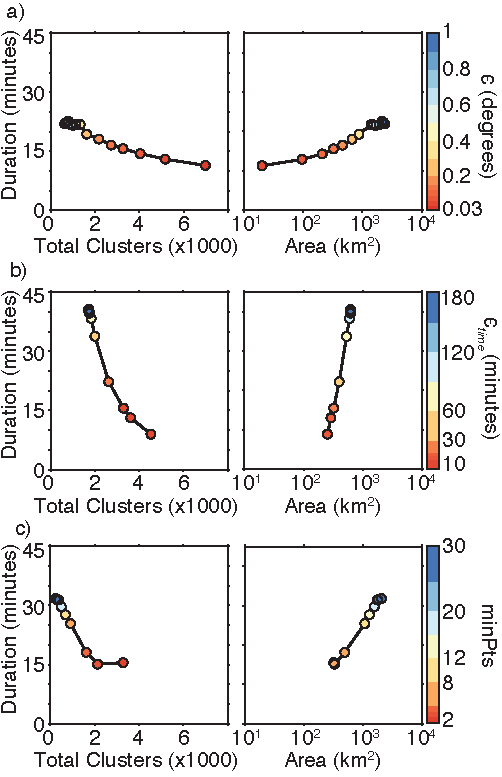
\includegraphics[scale=1]{GEC/Figures/parameters.pdf}
    \caption{Variation in average thunderstorm duration (rows), counts (left column) and area (right column) through varying one clustering parameter with the others held constant (constant set: $\epsilon = 0.12^\circ$, $\epsilon_{time} = 18$~minutes, and $minPts = 2$).
    		 a) $\epsilon$ varies from $0.03^\circ$ -- $1^\circ$.
		 b) $\epsilon_{time}$ varies from 10 -- 180 minutes.
		 c) $minPts$ varies from 2 -- 30 strokes.
		 }
    \label{gec:fig:parameters}
 \end{figure}

\section{WWLLN thunderstorm clusters}

Using the DBSCAN algorithm the individual WWLLN lightning strokes from 2010 June - 2013 June are clustered into active thunderstorms.
Clustered WWLLN strokes allow for simple thunderstorm tracking as shown in Figure~\ref{gec:fig:evolution}; here the strokes comprising a thunderstorm are outlined with polygons every hour, and plotted with opacity increasing with time.
Figure~\ref{gec:fig:evolution} shows several active thunderstorms on 2013 May 21, 12 -- 23 UTC.
For clarity clustered thunderstorms with less than 50 strokes were removed from the plot.
The thunderstorm opacity increases at 8\% per hour with each color corresponding to a single thunderstorm cluster.

 \begin{figure}[ht!]
    \centering
    \includegraphics[scale=1]{GEC/Figures/evolution.pdf}
    \caption{Thunderstorm evolution from 2013 May 21, 12 -- 23 UTC.
    		 Polygons outline active lightning regions, colors correspond to thunderstorm cluster, opacity increases 8\%/hour.
		 For clarity, thunderstorms with less than 50 strokes were removed.}
    \label{gec:fig:evolution}
 \end{figure}

The cluster results can be directly compared to active precipitation regions as seen by the TRMM Precipitation Radar \citep{Kawanishi2000}.
Rainfall rates from the TRMM data product 2A25 were used as binned rates on a $0.25^\circ$ grid; in Figure~\ref{gec:fig:overpass} the TRMM rainfall data are shown as the background image, gray areas are not in view of the satellite.
WWLLN strokes are shown in Figure~\ref{gec:fig:overpass} if they occur between the start and end times of the TRMM regional overpass.

 \begin{figure}[ht!]
    \centering
    \includegraphics[scale=1]{GEC/Figures/overpass.pdf}
    \caption{WWLLN thunderstorm clusters (identified by color) over TRMM precipitation rate (mm/Hr) for 2013 May 06, 15:49 -- 15:59 UTC (a), 17:28 -- 17:37 UTC (b), 2013 May 21, 10:04 -- 10:13 UTC (c), 11:42 -- 11:52 (d).
    		(a) and (b) are successive passes as are (c) and (d), cluster colors are contiguous between passes.
		Gray areas were outside the range of the TRMM radar.}
    \label{gec:fig:overpass}
 \end{figure}

In Figure~\ref{gec:fig:overpass} two sets of consecutive overpasses are used, the first on 2013 May 06 from 15:49 -- 15:59 UTC (\ref{gec:fig:overpass}a) and 17:28 -- 17:37 UTC (\ref{gec:fig:overpass}b), the second in on 2013 May 21 from 10:04 -- 10:13 UTC (\ref{gec:fig:overpass}c) to 11:42 -- 11:52 UTC (\ref{gec:fig:overpass}d).
These passes were selected as they passed over the same thunderstorms twice with an appreciable amount of lightning activity in view of the satellite.
Unlike Figure~\ref{gec:fig:evolution}, the clustered WWLLN strokes are shown as individual strokes in the thunderstorm with many of the strokes overlapping each other in the center of the clustered regions.
The clustered thunderstorms match up well with the TRMM precipitation regions and clearly track the same thunderstorm between the consecutive overpasses.
Thunderstorms continue, and are clustered by WWLLN, well after TRMM no longer observes the area (green thunderstorm in Figure~\ref{gec:fig:overpass}c and~\ref{gec:fig:overpass}d).
There were no previous or later TRMM overpasses of these thunderstorms.

\section{Global thunderstorm activity}

Original estimates of global thunderstorm activity show afternoon peaks in lightning activity for each of the major lightning chimney regions: the Americas, Africa/Europe, and Asia \citep{Wilson1921}.
The global averaged WWLLN thunderstorm clusters show the previously measured long term averaged diurnal behavior of the global electric circuit activity, with a diurnal variation of 36\%.
The three year average of thunderstorm activity is shown in Figure~\ref{gec:fig:carnegie} for different regions (\ref{gec:fig:carnegie}a), for thunderstorm type (\ref{gec:fig:carnegie}b), and for seasons (\ref{gec:fig:carnegie}c), with the global average displayed in each panel (black).
Averages of thunderstorm activity are calculated from the total number of unique thunderstorms every 30~minutes.

 \begin{figure}[ht!]
    \centering
     \includegraphics[scale=1]{GEC/Figures/carnegie.pdf}
    \caption{Diurnal variation of WWLLN thunderstorm 30~minute counts for 2010 -- 2013 obtained using the DBSCAN clustering algorithm.
    		 For a) thunderstorms over each major lightning chimney region (divided between longitudes $-180^\circ$, $-30^\circ$, and $60^\circ$),
		 b) all, land, ocean, and coastal thunderstorms (coastal thunderstorms have strokes over land and ocean),
		 and c) the full year and each season.
		 }
    \label{gec:fig:carnegie}
 \end{figure}

Each chimney region is separated in Figure~\ref{gec:fig:carnegie}a with peaks in thunderstorm activity occurring in the local afternoon (Americas 19~UTC, Africa 15~UTC, and Asia 8~UTC) then a slow decrease during the night until a minimum in the early hours of the morning.
A strong diurnal variation is evident for thunderstorms over land, seen in Figure~\ref{gec:fig:carnegie}b, with  little diurnal variation in oceanic thunderstorm activity.
On average WWLLN observes a total of $660 \pm 70$ thunderstorms on any given day of the year; while the total is lower than previous estimates in the 1000 -- 2000 thunderstorm range, those estimates were made using partial or extrapolated datasets.
For each chimney region the average number of thunderstorms are $280 \pm 80$ for the Americas, $140 \pm 60$ for African and Europe, and $240 \pm 50$ for Asia and the Maritime Continent.
The long-term thunderstorm behavior observed by WWLLN resembles the previous measurement of global electric circuit behavior.
Of the clustered thunderstorms $350 \pm 70$ were continental and $300 \pm 10$ were oceanic.
This is in contrast to the disparity in the distribution of individual lightning strokes where a majority are continental; the continental thunderstorms tend to be larger with higher stroke rates than those over the oceans.

There are slight changes in the overall diurnal behavior between each season shown Figure~\ref{gec:fig:carnegie}c.
The contribution of each chimney region, divided by northern and southern hemisphere, is shown in Figure~\ref{gec:fig:bimonthly}.
The overall seasonal change in thunderstorm activity is clearly seen with the change in dominant contributor from the northern hemisphere in May -- August to the southern hemisphere in November -- February.
In the shoulder seasons (March -- April and September -- October) the different chimneys are closer in activity levels to each other.
The shift in peak activity times for each chimney region between northern and southern summer reflects the difference in longitudinal landmass distribution of each region.
For example the North America peak occurs at 23:30 UTC while the South America peak occurs at 18:30 UTC since the South American lightning regions are, in general, farther east than the North American ones.
This time change in regional contributions has been seen in other global circuit measurements; in the Vostok, Antarctica electric field measurements of the fair weather field, the peak changes from 18:00 UTC in January to 21:00 UTC in August \citep{Burns2005, Burns2012}.

 \begin{figure}[ht!]
    \centering
    \includegraphics[scale=1]{GEC/Figures/bimonthly.pdf}
    \caption{Diurnal variation of WWLLN thunderstorms for each major chimney region (colors) divided by hemisphere (Northern Hemisphere solid line, Southern Hemisphere dashed line).
    		Each panel shows two months of thunderstorm clusters averaged over 2010 -- 2013.
		 }
    \label{gec:fig:bimonthly}
 \end{figure}

\section{Temporal thunderstorm activity}

As a result of a constantly growing number of WWLLN stations, the number of WWLLN strokes detected increases with time due to improvements in the network and the detection efficiency.
As a result long term tracking of stroke rate  cannot be used without deconvolving detection efficiency improvements.
However thunderstorm counts have remained relatively constant while stroke rate has increased; WWLLN has been capable of detecting almost every thunderstorm since 2005 \citep{Jacobson2006c}.
In Figure~\ref{gec:fig:timescale}a the daily average 30~minute thunderstorm counts (black) are plotted alongside the daily average stroke rate (red).
It can been seen that the stroke rate has increased relatively steadily while the thunderstorm count has remained relatively stable.

 \begin{figure}[ht!]
    \centering
    \includegraphics[scale=1]{GEC/Figures/timescale.pdf}
    \caption{Variation in WWLLN thunderstorm count (black) and stroke rate (red) for:
    		a) daily averages 30~minute counts from 2010 June -- 2013 June,
		b) 30~minute counts from 2011 June 01 -- 30,
		c) 5~minute counts from 2011 June 15, 00 -- 23 UTC.}
    \label{gec:fig:timescale}
 \end{figure}

The daily average thunderstorm count remains relatively constant during 2010 -- 2013, while the stroke rate increases during the same time span.
The thunderstorm count increased an average of 3\% per year, while the stroke had a much higher yearly increase of 13\%.
Similarly 90\% of the daily thunderstorm averages are within 20\% of the mean for the three years.
Previous work has suggested that changes in climate will cause a change in global thunderstorm behavior \citep{Williams2005a, Price2009a}.
During 2010 -- 2013 the average global surface temperature and thunderstorm count have both remained relatively constant \citep{Hansen2013a}, but future changes in global temperature may be reflected in the global average thunderstorm count.

Figure~\ref{gec:fig:averaging} shows that the typical diurnal behavior of Figure~\ref{gec:fig:carnegie} emerges only after long term averaging.
When examining the thunderstorm counts on a monthly scale (Figure~\ref{gec:fig:averaging}, dot-dash line) the long term average begins to emerge, while over a single day (Figure~\ref{gec:fig:averaging}, dashed line), the expected diurnal behavior is missing.
Similarly, on the daily scale of Figure~\ref{gec:fig:timescale}c it can be seen clearly that stroke rate does not follow thunderstorm counts as located by WWLLN.
Despite the short time scale variation, the overall average of the data still accurately reproduces the expected global thunderstorm activity in Figure~\ref{gec:fig:carnegie}.
With such short time scale variations global observations of the global electric circuit source mechanism, be it with ground lightning networks or several geostationary satellites, need to occur along with an accurate measure of the return current to better understand the charging of the global electric circuit.

 \begin{figure}[ht!]
    \centering
    \includegraphics[scale=1]{GEC/Figures/averaging.pdf}
    \caption{Diurnal UTC variation in WWLLN 30~minute thunderstorm count for:
    		multi-year average of Figure~\ref{gec:fig:timescale}a (solid line),
		monthly average of Figure~\ref{gec:fig:timescale}b (dot-dash line),
		and 30~minute averages of Figure~\ref{gec:fig:timescale}c (dashed line).}
    \label{gec:fig:averaging}
 \end{figure}

\section{Global Electric Circuit Thunderstorm Contribution}

With the WWLLN thunderstorm clusters a simple model is made to estimate the total contribution of thunderstorms and electrified storm clouds to the global electric circuit.
\citet{Mach2011} considered LIS/OTD observed land thunderstorms with less than 1.7 flashes min$^{-1}$ and ocean thunderstorms with less than 0.33 flashes min$^{-1}$ electrified storm clouds.
For an average storm duration of 15~minutes these cutoffs are 26 flashes for land and 5 flashes for oceanic electrified storm clouds (ESCs).
With a WWLLN-LIS/OTD detection efficiency of 6.4\% over land and 17\% over oceans \citep{Rudlosky2013}, WWLLN would expect cutoffs of 2~strokes per thunderstorm over land and 1~stroke per thunderstorm over oceans.
Given the clustering parameters used in this work requires a minimum of 2~strokes to be considered a thunderstorm, every un-clustered WWLLN stroke is considered a single ESC.
The daily average of thunderstorms and ESCs observed by WWLLN are shown in Figure~\ref{gec:fig:wilson}a.
Since not all ESC will produce lightning the counts shown in Figure~\ref{gec:fig:wilson}a should be considered a low estimate.

  \begin{figure}[ht!]
    \centering
    \includegraphics[scale=1]{GEC/Figures/wilson.pdf}
    \caption{A simple model of the total global electric circuit current with contributions from land thunderstorms (green solid), oceanic thunderstorms (blue solid), land electrified storm clouds (green dashed), and oceanic electrified storm clouds (blue dashed).
    		a) shows the counts for each group and b) the current contribution to the total (black line).
		}
    \label{gec:fig:wilson}
 \end{figure}

The average thunderstorm and ESC current contribution is taken from the overflight data of \citet{Mach2010}.
Average current contribution for land thunderstorms is 1.0~A, for oceanic thunderstorms 1.7~A, for land ESCs 0.41~A, and for oceanic ESCs 0.13~A.
The total current for each contributor and the total current is shown in Figure~\ref{gec:fig:wilson}b.
The average thunderstorm current is found to be $1090 \pm 70$~A with a total peak-to-peak variability of 24\%.
The largest contributor are oceanic thunderstorms (47\%) with $510 \pm 10$~A, followed by land thunderstorms (32\%) with $350 \pm 70$~A; overall ESCs contribute 21\% to the thunderstorm global circuit current.

With a similar model based on the TRMM LIS/OTD data, \citet{Mach2011} found ocean thunderstorms contribute 32\% and land thunderstorms 55\%, with a total ESC contribution of 13\% to the total mean current of 2.04~kA.
Their difference in current and contributing fraction stems from an increased count of land thunderstorms.
This highlights a shortcoming of this simple model: land thunderstorms tend to be larger than oceanic storms; thunderstorm area should be taken into account along with overall counts.
However to validate any global circuit model a comparison needs to be made with simultaneous fair weather return current measurements in order to constrain the models.

\section{Conclusion}

Global thunderstorm count is a good measure of global electric circuit activity and for a simple model of the circuit; the location and size of thunderstorms is necessary along with totals to create a more accurate model of the real time fair weather return current.
WWLLN strokes are successfully clustered into thunderstorms using the DBSCAN clustering algorithm with appropriately chosen clustering parameters.
The clustered thunderstorms were compared against the TRMM Precipitation Radar and a case study of thunderstorm tracking and evolution.
When the three years of WWLLN data were averaged the diurnal behavior of global thunderstorm activity aligned with the expected behavior of both thunderstorms and the fair weather return current.
The results of global thunderstorm and electrified storm cloud activity are combined with upward thunderstorm current averages to create an estimate of the fair weather return current.
The model found an average thunderstorm current contribution of $1090 \pm 70$~A.
This, and future, estimates of the current can be validated against an accurate fair weather return current measurement.

\subsection*{Acknowledgments}
The TRMM data used in this effort were acquired as part of the activities of NASA's Science Mission Directorate, and are archived and distributed by the Goddard Earth Sciences (GES) Data and Information Services Center (DISC).


% ========== Thunderstorms

\chapter{Thunderstorms and Flashes}
\label{thesis:chapter:thunderstorm}

\section{Overview}

Application of clustering algorithms to ground based lightning detection networks expands the real time global observations of lightning from strokes to flashes and strokes to thunderstorms.
Lightning detection networks, such as WWLLN or ENTLN, are then able to identify, locate, and analyze nearly every active thunderstorms within their operational range.
Global thunderstorm information allows for research into the climatological structures of thunderstorm behavior on large spatial and temporal scales.
Flash clustering allows for new network diagnostics, such as flash multiplicity and thunderstorm detection efficiency.

The DBSCAN algorithm is used to cluster strokes to flashes and thunderstorms for both the WWLLN and ENTLN.
Cross validation of the networks is performed with the located thunderstorms and comparisons of their inferred areas and duration.
Overall WWLLN detects 61\% of all ENTLN thunderstorm clusters and 80\% of thunderstorms larger than $10^3$~km$^2$.
In the reverse analysis, ENTLN detection of WWLLN thunderstorms, ENTLN detects 86\% of all WWLLN thunderstorms over North America.
On average WWLLN observes thunderstorm clusters lasting 10~minutes and spanning 66~km$^2$, ENTLN observes averages of 10~minutes and 60~km$^2$.
Within thunderstorms the average time between flashes is 21~seconds as seen by WWLLN and 10~seconds by ENTLN, with a strong dependence on season.
Clustering algorithms applied to lightning detection networks allow for a new range of analysis from thunderstorm effects, network performances, to the links between lightning and thunderstorms properties.

Lightning network detection efficiency is often measured in terms of relative stroke or flash performance through pair-wise comparisons of different systems.
For example comparing two ground based networks \citep{Abarca2010}, a ground based network with a satellite \citep{Rudlosky2013}, or a network to an actual ground truth such as rocket-and-wire triggered lightning \citep{Nag2011}.
In some cases, such as examining the global electric circuit (\citet{Hutchins2014}, Chapter~\ref{thesis:chapter:gec}), it is the location and properties of the thunderstorms generating the lightning that are important.
%% Add in some more thunderstorm important studies, see what cites Jacobson2006c
The thunderstorm detection efficiency for a lightning location system is then important in these applications, both the location, duration, and extent of the thunderstorm.

Within known thunderstorms the time between successive flashes can be used to examine further properties of the thunderstorm such as charging rate, controls on lightning strength, life cycle, and dynamics of the thunderstorm.
\citet{Zoghzoghy2013} examined the effect of the time between flashes as a measure of thunderstorm discharging in terms of the supression of future flashes.
\citet{Zipser1994} examined the relation between the flash rate in a thunderstorm with the updraft velocities, which in turn are controlled by the differential surface heating below the thunderstorm.
Only after considering and validating the performance of the lightning detection networks used can the effects of a flash be directly related to properties and behaviors of the parent thunderstorm.
Inferring thunderstorm properties based on the observed lightning flash rates can benefit regions with low availibility of direct or continuous observations (e.g. radar over oceans).

\section{Data}

%% Line about the detection efficiency?

The global WWLLN data will be used everywhere in this work unless specifically restricted to a given region, the ENTLN data will only be the North American subset of the data.
The data is from 2011 and 2012, with the exception of Section~\ref{thunderstorm:sec:interflash} which extends through June 2013.

\section{Methods}

Clustering the located strokes of both networks provides the thunderstorm and flash data.
The clustering is performed with the DBSCAN algorithm \citep{Ester1996, Kriegel2011a} following the application metholodgy discussed in Chapter~\ref{thesis:chapter:gec} \citep{Hutchins2014}.
DBSCAN is used over other clustering methods as it clusters based on the spatial and temporal distance between strokes with robust handling of noise (e.g. nearby thunderstorms).
The flash clustering uses the same algorithm as the thunderstorm clustering, with adjustment of the spatial and temporal clustering parameters.

For thunderstorms, WWLLN strokes are clustered together if they occur within $0.5^\circ$ and 18~minutes; for ENTLN it is $0.25^\circ$ and 15~minutes.
The tighter restraints on the ENTLN clustering stem from the higher density of strokes seen by ENTLN compared to WWLLN.
For flash clustering the strokes of both networks are clustered if they are within $0.12^\circ$ and 1~second of each other.
The 1~second timing is based on the natural inflection point observed in the WWLLN data (see Figure~\ref{thunderstorm:fig:interflash} in Section~\ref{thunderstorm:sec:interflash}).

The thunderstorm area is estimated by the best fit ellipse encapsulating all of the strokes in the cluster.
This will not be the areal extent of the thunderstorm system, rather just the electrified lightning region of the thunderstorm.
Similarly, thunderstorm duration is taken to be the time from the first stroke in a thunderstorm cluster to the last.
With these thunderstorm clustering parameters both networks observe similar average thunderstorm size and durations over North America.
WWLLN observes a median area and duration of 66 km$^2$ and 10~minutes, while ENTLN observes an average of 60 km$^2$ and 10 minutes.

A parameter used throughout this chapter is the time between successive strokes and flashes.
This interstroke time will refer to the time since the previous stroke in the parent thunderstorm cluster, while interflash time will refer to the time since the start of the previous flash in the thunderstorm cluster.

\section{Detection Efficiency}

The WWLLN thunderstorm detection efficiency is examined by comparing the located thunderstorm clusters with those located by ENTLN.
ENTLN does not have 100\% detection efficiency of strokes, it is used as a readily available baseline to compare to as a nominal ground truth for WWLLN.
Two thunderstorm clusters are considered to be matches if the convex hull of their constituent strokes overlap to within 5~km and $\pm5$~minutes.
Using a convex hull method requires at least three strokes in a thunderstorm for it be considered for a match; this creates an artifically lower detection efficiency for WWLLN for the cases where only 1 -- 2 strokes are detected in a thunderstorm.

Over the 2011 -- 2012 period in North America the average thunderstorm detection efficiency of WWLLN compared to ENTLN was 61\% while ENTLN has a detection efficiency of WWLLN of 86\%.
Similar to how detection efficiency varies with stroke strength, WWLLN has a higher detection efficiency of larger thunderstorms than smaller ones.
The spatial distribution of the detection efficiency is shown in Figure~\ref{thunderstorm:fig:deMap}.
In the southern regions, where there is typically higher thunderstorm activity, WWLLN has a detection efficiency above 70\%.
In regions with few thunderstorms (e.g. the West) there is a lower detection efficiency, possibly due to a lower detection efficiency of ENTLN in that region.

\begin{figure}[ht!]
   \centering
   \includegraphics[scale=1]{thunderstorm/Figures/deMap.pdf}
   \caption{WWLLN detection efficiency of ENTLN thunderstorms over North America for 2011 -- 2012 (top panel), with each season broken out in the lower panels.}
   \label{thunderstorm:fig:deMap}
\end{figure}

The seasonal behavior shows a similar overall distribution of detection efficiency, with an overall increase in winter (DJF) and spring (MAM) compared to summer (JJA) and fall (SON).
A winter increase, 68\% compared to 56\% in summer, is tied to the decreased occurrence of thunderstorms during the cold season.
In all seasons WWLLN has the highest detection efficiency over the oceans.
Increased detection efficiency at the limits of the ETNLN detection range (e.g. in the center of the Atlantic Ocean) is convolved with the decreased efficiency of ENTLN and not solely an increase in the WWLLN detection efficiency.

The daily spatially averaged detection efficiency is shown in Figure~\ref{thunderstorm:fig:deDaily}.
Here the seasonal variation is  evident; the high levels of noise in the winter reflects the lower overall thunderstorm counts during these months.
Within the annual variation, the detection efficiency does not vary with thunderstorm area, size, or duration; there is only a constant overall change in detection efficiency for all thunderstorm types.

\begin{figure}[ht!]
   \centering
   \includegraphics[scale=1]{thunderstorm/Figures/deDaily.pdf}
   \caption{Spatially averaged detection efficiency of ENTLN thunderstorms over North America.}
   \label{thunderstorm:fig:deDaily}
\end{figure}

The temporal distribution of thunderstorm detection efficiency can be split into different thunderstorm sizes (Figure~\ref{thunderstorm:fig:deBroken}a), total counts (Figure~\ref{thunderstorm:fig:deBroken}b), and durations (Figure~\ref{thunderstorm:fig:deBroken}c).
The daily detection efficiency increases for larger, productive, and longer thunderstorms.
For thunderstorms larger than $10^2$ km$^2$ the detection efficiency is 53\%, while for those larger than $10^3$ km$^2$ it is 80\%.
In a similar vein, thunderstorms with more than $10^2$~strokes are detected with 75\% efficiency and for more than $10^3$~strokes at 94\% efficiency.
Almost all thunderstorms observed are less than 1 hour in duration (Figure~\ref{thunderstorm:fig:deBroken}c, right), for those lasting more than 2 hours the detection efficiency increases to 93\%.


\begin{figure}[ht!]
   \centering
   \includegraphics[scale=1]{thunderstorm/Figures/deBroken.pdf}
   \caption{Temporal variation in thunderstorm detection efficiency for different thunderstorm sizes: a) thunderstorm area, b) thunderstorm stroke counts, and c) thunderstorm duration.
           The distribution of thunderstorms for each parameter is shown in the right panels.}
   \label{thunderstorm:fig:deBroken}
\end{figure}

Removing the temporal variation demonstrates the trend of increasing detection efficiency for each thunderstorm parameter.
In Figure~\ref{thunderstorm:fig:deParameter} the black lines represent all thunderstorms and the colored lines split the thunderstorms by total counts detected by WWLLN in these thunderstorms.
Thunderstorm area, Figure~\ref{thunderstorm:fig:deParameter}a, shows a gradual increase in detection efficiency from 40\% to near 100\% efficiency above $10^3$ km$^2$; the total number of strokes does not have an independent effect from area of the thunderstorm.
Similarly the longer a thunderstorm is active the more likely it is to be detected by WWLLN, shown in Figure~\ref{thunderstorm:fig:deParameter}c.
Unlike area, this is convolved with the size and count of the thunderstorm: smaller thunderstorms have lower detection efficiency regardless of duration and larger thunderstorms are easier to detect.

\begin{figure}[ht!]
   \centering
   \includegraphics[scale=1]{thunderstorm/Figures/deParameter.pdf}
   \caption{Thunderstorm detection efficiency for different thunderstorm a) areas, b) stroke counts, and c) durations.
           Area and duration plots are shown with the overall average (black) and for different total stroke counts (colors) within the thunderstorms.}
   \label{thunderstorm:fig:deParameter}
\end{figure}

%% I don't like the first "shows" in this sentence.
Matching thunderstorms between the networks shows the overall performance of the networks but not how the characteristics of the thunderstorms differ between the two networks.
If the thunderstorm clusters are capturing intrinsic properties of the thunderstorms independent of the overall detection efficiency, then the properties should be same between both networks.
For example, if WWLLN measures a thunderstorm to have an area of 66~km$^2$ with 50~strokes and ENTLN measures an area of 60~km$^2$ with 200~strokes it can be said that both measure the actual estimated area of the thunderstorm cluster.
%% This needs to be better

The properties of the matched thunderstorm  between WWLLN and ENTLN can be directly compared for thunderstorm area and duration.
Density plots of the two networks estimation for each matched thunderstorm are shown in Figure~\ref{thunderstorm:fig:deSim}, where the counts in each bin are displayed on a log scale.
Each characteristics in Figure~\ref{thunderstorm:fig:deSim} shows a strong distribution along a single 1-to-1 line.
Area, Figure~\ref{thunderstorm:fig:deSim}a, has good agreement between both networks with 46\% of matches within $\pm25\%$ of each other; there is increased deviation for smaller thunderstorms compared to larger ones.
The WWLLN overestimation compared to ENTLN thunderstorm area may be caused by incorrect matches or accidental merging between two thunderstorm clusters.
The thunderstorm duration has the stronger relation of the two parameters, with 33\% of matches falling within $\pm25\%$ of the 1-to-1 line.
There is fairly good agreement between the two networks on thunderstorm properties despite the differences in overall detection efficiency.

\begin{figure}[ht!]
   \centering
   \includegraphics[scale=1]{thunderstorm/Figures/deSim.pdf}
   \caption{Thunderstorm comparison of matched thunderstorms for WWLLN and ENTLN for a) area and b) duration.
           Note: the density levels are on a log scale.}
   \label{thunderstorm:fig:deSim}
\end{figure}


The overall detection efficiency of WWLLN for ENTLN thunderstorms is lower than previous estimates of the networks thunderstorm detection performance, in this case it likely stems from only 67\% of WWLLN strokes clustered into thunderstorms.
The remaining 33\% of total strokes would increase the overall detection efficiency of thunderstorms for the cases where only 1 -- 2 WWLLN strokes match ENTLN thunderstorms.
In contrast ENTLN had 96\% of stroke clustered into thunderstorms due, in part, to the higher overall efficiency of the network.
The identified WWLLN thunderstorms exhibited similar characteristics to their corresponding ENTLN thunderstorms.

\section{Flash Clusters}
\label{thunderstorm:sec:interflash}

Within a thunderstorm cluster lightning detection networks are able to measure two additional properties: the interstroke and interflash timing.
The full WWLLN interstroke time, Figure~\ref{thunderstorm:fig:interflash}a, naturally shows two distinct peaks: one at 40~ms and another at 100~seconds with a natural inflection at 1~second.
With ENTLN the interstroke distribution does not show the same distinct peaks (Figure~\ref{thunderstorm:fig:interflash}c); because it is able to locate more strokes in each flash, the tail of the interstroke time distribution overlaps the interflash time distribution.
In the WWLLN interevent time distribution there is a spike of events near 10~$\mu$s caused by the same event recorded twice by the network, this also occurs less frequently with ENTLN.

\begin{figure}[ht!]
   \centering
   \includegraphics[scale=1]{thunderstorm/Figures/interflash.pdf}
   \caption{The interevent times for WWLLN (a) and ENTLN (c) and the interstroke (black) and interflash (blue) time distributions for WWLLN (b) and ENTLN (d).
           The dashed lines correspond to the best lognormal fits of the distributions.}
   \label{thunderstorm:fig:interflash}
\end{figure}

After the network events are clustered into flashes the time distributions can be split into the time between strokes in the same flash (black) and time between flashes (blue), shown in Figure~\ref{thunderstorm:fig:interflash}b and~\ref{thunderstorm:fig:interflash}d.
The stroke and flash distributions can be fit as lognormal distributions for each day of the year, an example set of fits is shown with the dashed lines in Figure~\ref{thunderstorm:fig:interflash}b and~\ref{thunderstorm:fig:interflash}d.
This fitting allows for the daily tracking of the interstroke (Figure~\ref{thunderstorm:fig:stability}a) and interflash (Figure~\ref{thunderstorm:fig:stability}b) times for both networks.
With WWLLN the global distributions (black) remain relatively centered at 71~ms and 100~seconds; over North America WWLLN averages (blue) are 60~ms for interstroke and 39~seconds for interflash times.
ENTLN (red) has lower daily averages of 53~ms and 17~seconds due to the higher detection efficiency.
The North American WWLLN distribution more closely matches the seasonal behavior present in the ENTLN distribution with a small offset in timing.

\begin{figure}[ht!]
   \centering
   \includegraphics[scale=1]{thunderstorm/Figures/interflashStability.pdf}
   \caption{Peak of interstroke (a) and interflash (b) times for WWLLN (black), WWLLN over North America (blue), and ENTLN (red).
          Points beyond $2^{th}$ and $98^{th}$ percentiles shown as dots for WWLLN North America and ENTLN.}
   \label{thunderstorm:fig:stability}
\end{figure}

Directly comparing the time evolution of a thunderstorm will not work with thunderstorms of differing durations.
To account for this the thunderstorm life cycle is normalized by the duration of the thunderstorm.
Each thunderstorm is broken into 9 time segments where the first flash in the thunderstorm is at time~1 and the last flash at time~9.
With this normalization the average interflash time is found at each step for all thunderstorm clusters located by the two networks, shown in black in Figure~\ref{thunderstorm:fig:timerate}.
The interflash time can be seen to decrease to the center of a thunderstorms life cycle before increasing at the end, this is consistant with the known life cycle of a thunderstorm.
The interflash time for different energy (Figure~\ref{thunderstorm:fig:timerate}a) and absolute peak current (Figure~\ref{thunderstorm:fig:timerate}b) deciles are also shown.

\begin{figure}[ht!]
   \centering
   \includegraphics[scale=1]{thunderstorm/Figures/stormTimeRate.pdf}
   \caption{The interflash time for time-normalized thunderstorms for WWLLN (a) and ENTLN (b), with times shown for all flashes (black) and by stroke strength decile bins.
     WWLLN strength is divided by flash energy and ENTLN by absolute peak current.}
   \label{thunderstorm:fig:timerate}
\end{figure}

All flashes follow the same behavior, regardless of energy or peak current, however there are offsets in interflash time for different strength strokes.
As seen with WWLLN, Figure~\ref{thunderstorm:fig:timerate}a, the interflash time increases for more energetic strokes; for ENTLN, Figure~\ref{thunderstorm:fig:timerate}b, the interflash time increases for absolute peak current.
Between normalized time~1 and~5 the interflash time for the 90$^{th}$ percentile and above stroke strengths decreases by 9\% for WWLLN and 17\% for ENTLN compared to the median interflash time.
This shows that longer times between flashes results in stronger flashes; more charge separation can occur in the thunderstorm resulting in the stronger flashes.
In Figure~\ref{thunderstorm:fig:timerate} the separation between different flash strengths is consistant at all points in the thunderstorm life cycle.
It is not a constant offset but increases at the weaker stages of the thunderstorm (beginning and end) where longer time is necessary for a stronger flash, caused by a decreased charge separation rate.
The time between flashes is one of the main controlling factors in the strength of the resulting flash.
%% Speculation: over 9000

\section{Conclusion}

%% Discussion of the detection efficiency

When compared to ENTLN, WWLLN performs better when detecting large and active thunderstorm regions.
The lower performance for smaller thunderstorm clusters may be due to the cutoff in the clustering that requires at least 3 strokes for a cluster, removing 39\% of strokes from the analysis.
Including these strokes would lead to less robust matches between the networks and conflate a stroke to thunderstorm detection efficiency and the thunderstorm to thunderstorm detection efficiency.
For the thunderstorms WWLLN does detect, the characteristics of the thunderstorm are on par with those of ENTLN.

%% Discussion of flash clusters

On a global scale there is little change in the time between successive strokes and flashes within thunderstorms, but locally there are strong seasonal variations.
Both ENTLN and WWLLN observed the same seasonal variation in North America, with a small offset in their times based on the general detection efficiency differences in the networks.
The seasonal behavior shows a decrease in interflash times from the end of winter to the beginning of summer; thunderstorms in these times have higher flash rates compared to thunderstorms during the rest of the year.

The charging rate for thunderstorms evolves through the lifecycle of the thunderstorm, with the highest lighting flash rate during the middle of a thunderstorm.
The flash observed change in interflash time reflects the changes in the charging rate of the thunderstorm; the resulting flash stength depends on the charging rate and the total time charging between flashes.
If charging rate was constant with time than flash strength would be constant with interflash time through the life of a thunderstorm.
For a given charging rate the strength of the resulting flash depends on the time since the previous flash and the current thunderstorm convective activity.


% ========== Conclusion and Future Work

\chapter{Conclusion and Future Work}
\label{thesis:chapter:conclusion}

Over the course of this dissertation WWLLN has been expanded to include several new features: energy per stroke, relative detection efficiency, flash clustering, and thunderstorm clustering.
These new features have been developed alongside new research and analysis using WWLLN by itself or in conjunction with other systems.
Most of the research completed here naturally leads to future projects and research avenues that can be explored in the context of this work.
Several of the possibilites for research with WWLLN: network characterization, thunderstorms, the global electric circuit, and other lightning processes are discussed in this chapter.

\section{WWLLN Characterization}

The relative detection efficiency model developed in Chapter~\ref{thesis:chapter:efficiency} provides one view of the WWLLN network performance but it relies on several assumptions.
Either the model can be advanced to not rely on these assumptions or those assumptions themselves can be directly monitored.
The main assumption is that the distribution of lightning energy is the same everywhere; this was seen not to hold in Chapter~\ref{thesis:chapter:landsea} between land and oceanic thunderstorms.
The model can take into account the varying energy distributions, or the expected variance, through the variability of the observed regional energy distributions over time.

A promising method for examining the energy detection efficiency is to check how the measured energy values change when the station configuration changes.
For example, processing the energy data after artificially removing a few stations to quantify how the energy distributions change.
Compare the two energy distributions to the change in detection efficiency relative to a reference network (e.g. ENTLN or LIS) to better parameterize the model.

Similarly, the accuracy of the energy measurements themselves can be improved by adapting the energy per stroke processing to include multiple well calibrated WWLLN stations.
In the processing described in this work the entire network calibration is bootstrapped from one station; the addition of a second well calibrated station can improve the energy measurements and help quantify the regional variation in energy uncertainty.
This can address the uncertainty that is introduced in the station calibrations for stations far from the first station.

Finally other network characterizations can be developed based on the clustering results.
The number of thunderstorms, the average number of strokes per thunderstorm, average flash multiplicity, or time between flashes within a single thunderstorm can be routinely monitored for network health.

\section{Thunderstorms}

\subsection{Cluster Validation}

The thunderstorm clustering discussed in Chapter~\ref{thesis:chapter:gec} and~\ref{thesis:chapter:thunderstorm} can benefit from additional validation.
Two potential methods for validation are large scale comparisons to TRMM precipitation rates and case studies against regional weather radars.
The TRMM comparison would require grouping of the precipitation data to compare to the estimated thunderstorm extents.
Weather radar comparisons would provide detailed ground truth of the thunderstorm cluster areas and durations.
Further, weather radar would allow for a measure of thunderstorm tracking accuracy.

Aside from comparisons to other sytems the properties measured by the thunderstorm clustering can be tracked over spatial and temporal scales.
For example: the average thunderstorm duration interannual variability in a given region or the overall network observed thunderstorm area.
This can explore the changes in the clustering values and accuracy as the stroke rate detected by WWLLN changes with time.

\subsection{Parameterization}

Thunderstorm parameterizations are functional relationships between different properties of thunderstorms.
Using lightning detection networks allows for the development of these relationships that infer thunderstorm properties based on the observed lightning flash rates; of particular benefit for regions with low availibility of direct observations (e.g. radar, satellite).
\citet{Zipser1994} examined the relation between the flash rate in a thunderstorm with the updraft velocities, which in turn are controlled by the differential surface heating below the thunderstorm.
Parameterization of flash rate based on other observations has led to simple models of global lightning behavior, \citet{Price1992} used cloud height parameterization for flash rate.
These empirical parameterizations can help in the development and validation of models (e.g. \citet{Baker1999}) of thunderstorm electrification and enable or expand prediction of the global electric circuit, NO$_\text{x}$ production, and weather forecasting.
Investigating the parameterization of lightning behavior in relation to the properties of a thunderstorm on a large scale can create better and more robust parameterizations.
The WWLLN thunderstorm clustering can be compared to other networks and systems in order to develop and validate new parameterizations.

\subsection{Thunderstorm Properties}

The WWLLN thunderstorm clustering can be used to investigate global and regional thunderstorm properties and their distributions.
Thunderstorm area and duration are briefly discussed in Chapter~\ref{thesis:chapter:thunderstorm}, but can be explored in more depth and in more regions.
These two properties can be measured over different spatial and temporal scales.
For example the distribution of winter thunderstorms over the Sea of Japan, or the South American ``green ocean'' phenoma.

Alternativey more complex measures of thunderstorms can be developed: the average stroke count per thunderstorm, the peak flash rate, or the electrical activity.
The electrical activity can be measured as the total flash energy per unit area per unit time for the thunderstorm: the sum of measured flash energies within the thunderstorm.
This measure, and others, may be highly dependent on the network performance or may not be absolutely calibrated, however they can still allow for relative comparisons between thunderstorms in a limited temporal or spatial scope (e.g. North America in July 2013).

The thunderstorm dataset can also be advanced by classifying thunderstorms into different thunderstorm types.
While this may only work for small case studies it may be possible to use more advanced machine learning classifiers to automatically assign cloud types to thunderstorm clusters.

\section{Global Electric circuit}

The global electric circuit model presented in Chapter~\ref{thesis:chapter:gec} provides an estimate of the thunderstorm contribution to the circuit based on the WWLLN thunderstorm clusters.
It is shown that the model is able to reproduce the expected Carnegie curve over long time scales and has the capability to provide current estimates on shorter time scales.
The model can be improved for a more accurate measure of the current contribution, but without any validation it cannot be reliably used.

To improve the model there are several underlying assumptions that can be factored in.
The main one is that all thunderstorms produce the same upward current to the ionosphere regardless of their size or activity.
The estimates used in the model from \citet{Mach2010} can be scaled by either the thunderstorm cluster activity or the estimated cluster size.
Since the development of the model the thunderstorm cluster area was validated against ENTLN in Chapter~\ref{thesis:chapter:thunderstorm}, giving confidence to the area measurements.
The second assumption is that all thunderstorm currents are the same everywhere.
This assumption is harder to address as it relies on direct measurements of the current made in different regions.

Regardless of the model improvements made, the model needs to be compared against a ground truth measurement.
Further, comparison to a ground truth will allow for tuning of the model to better fit the observerd measurements; or if adjustments cannot be made then other components of the global electric circuit need to be included in the model.
For the ground truth a balloon campaign needs to be conducted to measure the fair weather return current over the span of one to several weeks.
With a reliable and clean measurements of the return current the model can be validated on a very short time scale instead of relying on long term averages.

\section{Other Lightning Processes}

WWLLN is able to measure and detect more than just the main discharge of a lightning stroke.
The network is able to directly detect terrestrial gamma-ray flashes (TGF) and their related strokes, it is also able to detect whistler waves at the individual stations.
For TGFs WWLLN has been used to geolocate the TGF itself and the originating thunderstorm \citep{Connaughton2010, Connaughton2013}.
WWLLN can be used to create an estimate of the global TGF production rate by comparing the detected TGFs with the lightning within view of one of the TGF satellites (e.g. FERMI or RHESSI).
With whistler waves an automated whistler detector running at the remote WWLLN stations could enable the creation of a large database of whistler waves.
Such a database could provide the means for investigations of the ionosphere and magnetosphere, especially if the detector is able to run on multiple WWLLN stations.










%
% ==========   Bibliography
%

%\nocite{*}   % include everything in the uwthesis.bib file
\bibliography{/users/michael/documents/ess/research/library}
\bibliographystyle{/users/michael/documents/ess/research/agu}


%
% ==========   Appendices
%

\appendix
\raggedbottom\sloppy

% ========== Appendix Code

\chapter{Code Repositories}
\label{thesis:appendix:code}

This appendix discusses the distribution of WWLLN data files on the Flash series of computers along with the storage locations of routine processing code.
The code locations are given in terms of both their active locations and as the source control repositories, managed using git (http://git-scm.com).

\section{File Storage on Flash Machines}

There are several types of WWLLN data files, summarized in Table~\ref{code:fileType}.
The example filenames given in the table are for 31 December 2013, 5:10 UTC.
Most of the file types, with exception of WB-files, are located on flash5 on one of two hard drives.
Data for the current year is stored on /wd2/ while previous years are stored on /wd3/.
Each file type has it's own directory, denoted Afiles, AEfiles, etc., with flat file structures (except for R-files).
R-files, due to the large number generated, are broken into yearly and monthly folders of the form: /wd2/R[YYYY]/R[YYYY][MM]
The R-file repository on flash5 differs from that of flashdat since the 2005 and 2006 data has been cleaned and organized into a consistent file hierarchy.
Some, but not all, of the WWLLN data file directories have been copied to the other flashes on a need-basis and so the other flashes should not be considered a backup of the flash5 dataset.

\begin{table}[h!]
\begin{center}
\caption{WWLLN Data Types}
\begin{tabular}{|p{.75in}|p{2in}|p{3.5in}|}

\hline
{\bf File Type} & {\bf Naming} &	{\bf Description} \\

\hline
\rule{0pt}{3ex}
R-files	& R20121231051000	&	Raw packets sent by stations\\ 

\hline
\rule{0pt}{3ex}
A-files	& A20121231.loc	&	Lightning locations generated in real time\\ 

\hline
\rule{0pt}{3ex}
AP-files	& AP20121231.loc	&	Location data with station and E-field data of each stroke solution, generated daily with relocate-B\\ 

\hline
\rule{0pt}{3ex}
AE-files	& AE20121231.loc	&	Location and stroke energy data, generated daily by Bootstrap (Chapter~\ref{ch:energy})\\ 

\hline
\rule{0pt}{3ex}
DE-files	& DE20121231.mat	&	Relative detection efficiency maps, as Matlab data (Chapter~\ref{ch:de})\\ 

\hline
\rule{0pt}{3ex}
S-files	& S201212310510.Seattle.loc	&	Waveform data for strokes located near a given station.\\ 

\hline
\rule{0pt}{3ex}
WB-files	& WB201212310510.dat	&	Continuos wideband field data output by toga -r\\ 

\hline
\rule{0pt}{3ex}
T-files	& T20130130.dat	&	Station packet count record, listed date is last date updated-r\\ 

\hline
\end{tabular}
\end{center}
\label{code:fileType}
\end{table}
 
An example line from each of the R, A, AP, and AE files are given below with descriptors for each file.
R-files are the simplest with each line containing three columns:

\begin{verbatim}
10      3000.015563     2668
\end{verbatim}

The first number is the station ID, the second is the seconds from the start of the hour, and the last is the root integrated square electric field at the station, in uncalibrated sound card units.
For A-files each line if of the form:

\begin{verbatim}
2013/01/31,16:18:54.103460,  9.0621,-117.8276, 19.9,  9
\end{verbatim}

The first six numbers are the date (YYYY/MM/DD) and UTC time of the stroke (hh,mm,ss).
The next two are the stroke location in degrees north latitude and east longitude.
The final two are the timing uncertainty in microseconds and the number of WWLLN stations that participated in the stroke location.
AP-files are similar to A-files with additional information after the stroke location:

\begin{verbatim}
2013/02/12,00:00:07.142335,-10.4622,  20.0863, 13.4,  5,17,600,19,2084,26,453,53,225,
	64,2263
\end{verbatim}

Starting at 17,600 are pairs of numbers that give the station ID (17) and the field strength (600) in sound card units, the same value as in the R-files. Finally AE-files are similar to A-files but with three additional numbers:

\begin{verbatim}
2013/2/12,00:00:07.142335, -10.4622,  020.0863, 13.4, 5, 448.86, 114.87, 4
\end{verbatim}

The last three numbers correspond to the radiated VLF stroke energy in joules (448.86), the median absolute deviation of the energy value in joules (114.87), and the subset of stations that participated in the energy value solution (4).

T-files are records of how many packets a given station sent to flash4 during the history of WWLLN.
Unlike the other files it is not automatically generated, rather it is written whenever it is updated through the TfileUpdater.m script in the functions.git repository.
Each line contains the date in days since 01/01/0000 and the counts for each station, where column 2 corresponds to station 0.

\section{Code Repositories}

All of my code should be stored on flash5 at /home/mlhutch/matlab for Matlab scripts.
For example the code to run the energy processing is located at /home/mlhutch/matlab/Bootstrap/bootstrap\_automation.m.
The exact details of where the energy processing code is located, the necessary files, and similar code for the relative detection efficiency processing is covered in Appendix~\ref{app:energy}.
Aside from being stored in plaintext scripts, all of the code is also stored in a Git repository located both on flash5 (/home/mlhutch/Git) and hosted online on bitbucket.org.

The Git repositories have the advantage of multiple back ups, version control, easily portable, and easy to use.
A list of the WWLLN processing code and corresponding git repository is given in Table~\ref{code:repo}.
A basic primer on how to use git, including retrieval of the repositories, is given in Section~\ref{code:primer}.

\begin{table}[h!]
\caption{Git Repositories (flash5:/home/mlhutch/Git/)}
\begin{center}
\begin{tabular}{|p{1.5in}|p{1.25in}|p{3in}|}

\hline
{\bf Code} &	{\bf Repository} &	{\bf Notes}\\

\hline
\rule{0pt}{3ex}
Energy Processing	&bootstrap.git	&	Requires process.git and functions.git \\ 

\hline
\rule{0pt}{3ex}
Detection Efficiency	&de.git	&	Requires functions.git\\ 

\hline
\rule{0pt}{3ex}
LWPC	&lwpc.git	&	LWPC and Matlab implementation\\ 

\hline
\rule{0pt}{3ex}
AP Processing	&process.git	&	Relocate files (required for energy processing)\\ 

\hline
\rule{0pt}{3ex}
MATLAB Functions	&functions.git	&	Various Matlab functions required by other scripts.\\ 

\hline
\rule{0pt}{3ex}
SU Eagle Files	&eagle.git	&	Eagle files for WWLLN SU and Pre-amps, includes Erin Lay's files.\\ 

\hline
\rule{0pt}{3ex}
Gumstix	&gumstix.git	&	Files for building and configuring Gumstix microSD cards.\\ 

\hline
\rule{0pt}{3ex}
Gumstix Bitbake	&openembedded.git	&	Bitbake distribution for adjusting Gumstix kernel\\ 

\hline
\end{tabular}
\end{center}
\label{code:repo}
\end{table}

\section{Git Primer}
\label{code:primer}

Git (http://git-scm.com) is an open source distributed version control system available on all operating systems with very little system resources required.
Most often git is accessed through the command line but there are many graphical interfaces available.
I chose git for my research and code since it allows easy branching, constant backups (locally and on remote servers), and helps to organize code and projects.
A brief tutorial on git is available online: http://git-scm.com/book/en/Getting-Started and http://try.github.com/.

Once git is installed on a host machine (http://git-scm.com, apt-get install git, or yum install git-core) repositories can be downloaded with the command:

\begin{verbatim}
git clone [user]@[server]:[repository] .
\end{verbatim}

This will copy (clone) the repository to the current directory as a folder of the same name as the repository. 
For example to copy over the energy processing repository listed in Table~\ref{code:repo} to the matlab directory:

\begin{verbatim}
cd ~/matlab
clone sferix@flash5.ess.washington.edu:/home/mlhutch/Git/bootstrap.git .
\end{verbatim}

Where the user can be anyone with permission to access that directory.
More information on how to use git for source control, instead of downloading the repositories, can be found in the online resources.
I am happy to have user collaborate with the flash5 git repositories for updates, changes, or additions to the listed repositories.

\section{Other Useful Matlab Code}


% ========== Appendix Bootstrap

\chapter{Energy Processing}
\label{thesis:appendix:energy}

The process for bootstrap calibrating the WWLLN stations and how the energy is calculated is described in \citet{Hutchins2012}.
This section walks through the code used in the processing along with the decisions behind various checks and adjustments made in the processing.

\section{Code Summary}

There are 8 main sections to the bootstrap processing:

\begin{itemize}
	\item{Process R-files into AP-files}
	\item{Calculate LWPC attenuation coefficients for each stroke-station pair}
	\item{Bootstrap calibrate the network}
	\item{Calculate stroke energy using LWPC and calibration}
	\item{Iterative re-calibrate the network}
	\item{Final energy calculation}
	\item{Run Relative Detection Efficiency Model (Chaper~\ref{thesis:chapter:efficiency})}
	\item{Move files to storage locations}
\end{itemize}

This processing requires several files, locations given relative to mlhutch@flash5.ess.washington.edu.

\begin{itemize}
	\item{\textbf{$\sim$/Process/relocate-B31Jan2013.x86-64} -- James Brundell's relocate program used to process R-files into AP-files, this version compiled for Linux 64-bit systems}
	\item{\textbf{stations.dat} -- list of current WWLLN stations, copied over from flash4 at the start every processing run.}
	\item{\textbf{lwpcv21} -- directory containing a working compiled version of the LWPC code.
		Used in generating new lookup tables as stations are added, a parallelized matlab implementation is discussed below.
		Provided as a sub-module of the Bootstrap directory.}
	\item{\textbf{$\sim$/matlab/Bootstrap/} -- directory containing the necessary matlab files, available as a git directory (see Appendix~\ref{thesis:appendix:code}).}
	\item{\textbf{$\sim$/matlab/functions/} -- directory of necessary matlab functions used by the Bootstrap code files, also available as a git directory (see Appendix~\ref{thesis:appendix:code}).}
\end{itemize}

\section{LWPC}

The Long Wave Propagation Capability code is a codebase developed by \citet{Ferguson1998} that is used to calculated the electric field at a given location for a VLF transmitter at another location.
For the WWLLN energy processing it is used to estimate the attenuation between a stroke (treated as a transmitter) and a station.
The original LWPC code has been altered in two ways: first the Windows-compiler specific code has been replaced with GCC compilable code, second all warning have been removed to produce output of a constant shape (for reading into MATLAB).
All edits in the source code have been marked by my initials of MH.

\subsection{Compiling}

To recompile LWPC two bash scripts need to be run.
The first is \textbf{BuildData.cmd}, BuildData recompiles the data files that contain the surface parameters such as ground conductivity and coastlines.
The second step is to run \textbf{buildlwpc.cmd}, this should compile the program and result in an executable called LWPC.
To test a successful compile run the script \textbf{run\_bench.cmd}, if it runs successfully it is compiled, if not consult the \textbf{Readme - Unix.txt} file that has some common troubleshooting steps.

The last step in setting up LWPC is to set the \textbf{lwpcDAT.loc} file to point towards the \textbf{data} folder.

\subsection{Running}

LWPC is run from the command line with the structure:

\begin{verbatim}
./LWPC test1.inp
\end{verbatim}

Where \textbf{test1.inp} is formatted as per the structure in \textbf{User\_manual.pdf}.
The matlab implemtations discussed below automatically generate formatted input files.

The result of running LWPC is an output file the specifies the electric field at various distance along the path from the transmitter to receiver.
It is also capable of outputting plots, azimuthal dependence, and many other features not utilized in this research.

\subsection{Matlab Function}

A matlab implementation of LWPC is available as a git repository (see Appendix~\ref{thesis:appendix:code}).
This implantation allows for LWPC to called in matlab with:

\begin{verbatim}
LWPCpar(freq,lat,long,time,stat_lat,stat_long,model)
\end{verbatim}

Where freq is the transmitter frequency, lat/long is the transmitter location, time is the date and time, stat\_lat/stat\_long are the receiver locations, and model is the ionospheric model used.
If model is set to ``time'' then day and night is considered in the calculation, if it is set to ``day'' or ``night'' an all day or all night ionosphere will be used.

LWPCpar as the advantage of being runnable within matlab parallelized loops (parfor).
While LWPC itself cannot be run in parallel, this method simply copies the LWPC directory to allow each matlab instance it's own copy.

\section{Lookup Tables}

While LWPC can be parallelized it is still too slow to run faster than realtime for WWLLN processing.
As a result two sets of lookup tables are generated for each station with the pre-calculated LWPC electric field values.

The lookup tables are part of the main Bootstrap directory under the names \textbf{lookup\_day.dat} and \textbf{lookup\_night.dat}.
Each of these files are tab-delimited text with the format given in Table~\ref{bootstrap:table:lookup}.
The tables list the electric field measured the the station given a 100~kW transmitter in each grid point on the globe.
The latest lookup tables are at a resolution of $2^\circ$.

\begin{table}[h!]
\begin{center}
\begin{tabular}{|p{1.5in}|p{1.75in}|p{1.75in}|p{1in}|}
\hline
\rule{0pt}{3ex}
Station Name	&Station North Latitude	&	Station East Longitude & \\ 
\hline
\rule{0pt}{3ex}
E-field at (-179,89)	& E-field at (-178,89) &	E-field at (-177,89) & \dots \\ 
\hline
\rule{0pt}{3ex}
E-field at (-179,88)	& E-field at (-178,88) &	E-field at (-177,88) & \dots \\ 
\hline
\rule{0pt}{3ex}
E-field at (-179,87)	& E-field at (-178,87) &	E-field at (-177,87) & \dots \\ 
\hline
\rule{0pt}{3ex}
\dots	& \dots &	\dots & \dots \\ 
\hline
\end{tabular}
\end{center}
\caption{Format for \textbf{lookup\_day.dat} and \textbf{lookup\_night.dat} data files for a resolution of $1^\circ$.}
\label{bootstrap:table:lookup}
\end{table}

An example of a lookup table for the all day ionosphere for Dunedin station is shown in Figure~\ref{bootstrap:fig:lookup}.

\begin{figure}[ht!]
   \centering
   \includegraphics[scale=1]{Introduction/Figures/lwpc_lookup.pdf} 
   \caption{Lookup table for an all day ionosphere for Dunedin station.}
   \label{bootstrap:fig:lookup}
\end{figure}

\subsection{Generation}

The LWPC lookup tables are generated automatically with the matlab script {\bf $\sim$/Bootstrap/\\Lookup\_automation.m} that is called at the start of the daily energy processing.
The script checks the current number of stations in the \textbf{.dat} files and compares it to the most recent \textbf{stations.dat} file.
If there are a new entries in the \textbf{stations.dat} then the script proceeds to make the lookup tables.

The automatic script calculates the electric field at every grid point for 11 frequencies ranging from 8~kHz to 18~kHz, and averages them together to add to the \textbf{.dat} files.

The same script can be run for specific stations with the \textbf{$\sim$/matlab/lwpcpar/lwpc\_generate.m} script.

Tables generated with either script can be validated with the \textbf{$\sim$/matlab/Bootstrap/\\lookup\_validation.m} scipt.
This script checks each grid point to ensure there is a real number there, sometimes LWPC generates errors for very specific locations.
If there is no valid electric field value at that spot it is reprocessed by offsetting the transmitter by a fraction of a degree.

\section{Matlab Code}

The main matlab script to run the entire energy calculation process is {\bf Boostrap\_automation.m}.
This script:
\begin{enumerate}
\item{Defines the dates to run (in case past days need to be rerun)}
\item{Sets the system path parameters from {\bf data\_path.m}}
\item{Updates stations.dat and the lookup tables {\bf Lookup\_automation.m}.}
\item{Generate the current AP-file with {\bf generate\_ap.m}}
\item{Calculate the energies and station calibrations using {\bf wwlln\_energy.m}}
\item{Generates the relative detection efficiency map with {\bf de\_mapper.m}}
\item{Calculates network statistics with {\bf network\_statistics.m}}
\item{Generate and amend T-files to TCurrent.dat}
\item{Saves and archives all of the resulting data files}
\end{enumerate}

In order to rerun lost days the only change necessary for Bootstrap\_automation is to change the rundate from:

\begin{verbatim}
		RUNDATE = floor(now - 1);
\end{verbatim}

to the day (or dates) that need to be rerun.
The LIVE variable and second part of the if clause is for rerunning \emph{previously processed} data.
If LIVE is set to false then the script runs and stores in an alternative directory with a copy of the resulting calibration file.
For the case of restarting the script on the same day it failed to run, no changes need to be made.

\subsection{data\_path.m}

It is important to correctly set up the {\bf data\_path.m} script. 
Aside from the storage paths, it is important to set how the script should obtain the stations.dat and R-files from flash4.
The transfer type can either be cp if the computer has flash4 network mounted, or scp if passwordless scp is setup.
The r\_path\_flat variable determines whether the R-files are stored in one directory or with a hierarchal structure (e.g. /wd2/Rfiles/R2013/R201304/R201304*).

Additionally the location of the bootstrap processing folder itself as well as the TOGA relocate script.

\subsection{Lookup\_automation.m}

The {\bf Lookup\_automation.m} script compares the current number of entries in the lookup\_day.dat data file and compares it to the latest stations.dat file.
If stations.dat has new entries, then the script generates the corresponding LWPC lookup tables for those new stations.

Using the current lookup spatial resolution LWPCpar is called for each grid point at 11 frequencies (8 -- 11~kHz) for both day and night.
The 11 values in each grid point (in dB) are averaged together and added to the existing lookup data files.

This code takes about twelve hours to run using a single core due to calling the LWPC code.
The LWPCpar.m function is set up to run in parallel (it copies the LWPC code to new locations), however the {\bf Lookup\_automation.m} script has not be parallelized.

\subsection{generate\_ap.m}

{\bf generate\_ap.m} copies over the R-files to the TOGA relocate folder and processes them with the -e flag.
This generate the normal WWLLN A-file structure, with the addition of the participating stations and their RMS electric field values at the end of each line.
The RMS electric field (as mentioned elsewhere) is in the uncalibrated sound card units, where the calibration is the main part of the wwlln\_energy.m code.
The script ends with moving the new AP file and R-files to their storage locations.

\subsection{wwlln\_energy.m}

The {\bf wwlln\_energy.m} function runs the subfunctions described below in order to calculate the stroke energies.
Unless it is set otherwise (which it should be), the script sets the default master station to use to be Scott Base with the most recent calibration.
The master station is one with a known calibration that is used to bootstrap the calibrations for the rest of the network.
One future upgrade to the code would be the ability to include multiple master stations and combine their results for a better system-wide calibration.

The script also generates and saves two sets of station ratios.
The first is the station conversion file, the values in this file give how to convert the sound card units at the master station to the sound card units at the other stations.
It is saved in the case that the master calibration requires a retroactive change.
The calibration file gives the values to convert from individual station sound card units to RMS electric-field values.
The station calibration incorporates both the actual station calibration and any environmental changes near the station.

{\bf apply\_lwpc.m} applies the LWPC lookup tables to each sound card value in each stroke-station pair.
The day and night lookup table values are weighted by the percent of the path in daytime and nighttime.
There is also a distance range restriction, where only stroke-station values between 1 and 8~Mm are calculated, otherwise they are given a value of zero.

{\bf cross\_calibration.m} finds all strokes common to each pair of stations, and uses them to create a conversion ratio between every pair of stations.
Only if the two stations have common strokes in all day paths and are within the same 1 -- 8~Mm distance restriction.
The median value of every common stroke value is used as the resulting station-pair conversion ratios.

{\bf bootstrap.m} solves the connected graph of station-pair conversions to find the valid calibration paths from the master station to every other possible station.
There are two ways for a station to be added as a well calibrated station.
First it can have common strokes between itself and the master station, this would result in a single hop conversion.
The second way is to be calibrated off of one of the previously calibrated stations.
In this case a secondary (or tertiary etc.) calibration is validated by comparing it's direct conversion with a conversion using it as an intermediary.
So to test if the calibration of A to B is valid, B is used in the A to B to C calibration.
If the ABC calibration matches the direct AC calibration to within 75\% then B is considered well calibrated.
This bootstrapping is conducted for 5 hops, so any converted station is at most 4 intermediary stations away from the master station.

{\bf conversion\_check.m} takes the resulting calibration paths from bootstrap.m and performs the bootstrap calibration using the initial calibration of the master station and the conversion ratios of cross\_calibration.m.
It also requires that the master station is included in the case where it becomes excluded in the bootstrap.m subfunction.

To prevent sudden changes in gain or wildly varying station from being included {\bf conversion\_mean.m} checks the new calibration values against the previous 7 days of calibrations.
If the new calibration is not drastically different then the average of the previous 7 days of calibration values is used as the calibration value, otherwise it is excluded.
A station is deemed unstable if one of the past seven days is either larger or smaller than the median by a factor of 10 (normalized by Scott Base, Dunedin, and Seattle).

{\bf stroke\_energy.m} applies the calibration values from conversion\_mean.m to the LWPC corrected data from apply\_lwpc.m to get the stroke energy.
The stroke energy is the median of the individual station values and the uncertainty is the median absolute deviation of the values.
The values are stored as the 11$^\text{th}$ and 12$^\text{th}$ column in the resulting AE-file.
The 13$^\text{th}$ value is the number of stations that participated in the calculation.

The final step is to iterate the entire process 5 times with {\bf energy\_iterate.m}.
Here the stroke energies are taken to be ground truths from which all of the calibration values are recalculated.
The new calibrations are then used in stroke\_energy.m to get a new set of energy calculations.
After 5 iterations the values start to converge and the resulting calibrations and values are used as the final values.
The iteration is performed to remove far outliers (2-4 order of magnitude larger or smaller than other values) and get a more stable result.

Once the final energy and calibration values are found, the data is written to both .loc and .mat files for the AE-files and the .txt files for the calibration and conversion values.
The conversion file is only used within the processing internally (and with reprocessing), for any station level calibration work the calibration file should be used.
Then the {\bf de\_mapper.m} function is called to get the relative detection efficiency for the day, the results stored as a DE-file.
Finally a set of network statistics are stored in a file for quick reference (currently this file is not being ingested or incorporated anywhere, such as the WWLLN management page).

\section{Relative Detection Efficiency Code}

The overall description of the relative detection efficiency model is given in Chapter~\ref{ch:de}.

\subsection{de\_mapper.m}

{\bf de\_mapper.m} creates the relative detection efficiency model for each hour in the day, currently the code is written such that this step is parallelized if the parallel toolbox is available and running.
Within each hour the subset of operational stations ($>500$ stroke solutions) are used to create the model.

For each station the stroke-station pairs are found that are between 0.5 -- 20~Mm, these are used to determine the station detection threshold for the current hour.
The threshold is determined as the 5th percentile value of the local electric field value (in uncalibrated soundcard units) from the stroke-station pairs.
This is converted into a minimum stroke energy for an array of potential attenuation rates to serve as a lookup table.
Using the current station calibration averaged over the past 7 days.

The {\bf terminator.m} program is used to determine the percent day and night paths between the station and every grid point on the globe.
These ratios are combined with the LWPC lookup tables to determine the attenuation at every grid point.
Finally the attenuation values are used to index the potential stroke energy lookup to get the minimum detectable stroke energy at each grid point.

After this is performed for each station the 5th lowest value is found at each grid point.
The 5th lowest is chosen as at least 5 stations are required to locate a WWLLN stroke, if that requirement ever changes then it would need to be changed in this code as well.
The 5th lowest value corresponds to the minimum detectable energy of the network for the given hour.

The minimum detectable network energy is compared to the energy distribution of the past 7 days.
For this distribution only strokes with energy solutions using 2 or more stations are totaled.
The percentage of strokes above the minimum is called the relative detection efficiency for that grid point.

\subsection{Output Interpretation}

The output of the model is a $n\times m \times 24$ array where $n$ and $m$ are determined by the resolution of the lookup tables.
For example if the lookup tables have a resolution of $2^\circ$, then $n=180$ and $m=90$.
The third dimension of the array corresponds to the UTC hours 0--23.

In each grid cell is the relative detection efficiency of the network on a 0--1 scale.
The 1 corresponds to locations that could detect 100\% of the past 7 day distribution and are the best performing regions of the network.
Other locations will have values below 1\%, such as Antarctica.
It is recommended that prior to use a minimum relative detection efficiency, such as 5\%, is set on the maps to prevent unphysical stroke density counts.

In the automated Boostrap processing the resulting relative detection efficiency maps are expanded to a $1^\circ$ grid and smoothed to give a standardized size in the case that the lookup tables change their resolution.
In the unlikely case that the resolution goes below $1^\circ$ the maps should then be downsampled to recreate this resolution.

% ========== Appendix Service Unit

\chapter{WWLLN Service Unit v4}
\label{thesis:appendix:su}

\section{New Design}

The WWLLN service unit was redesigned due to the obsolescence of the previous Trimble GPS unit, this redesign allowed for several other major revisions to the board:

\begin{itemize}
\item{Built in USB-Serial conversion}
\item{On board computer}
\item{Remote controlled pre-amp power system}
\item{Remove inline preamp LEDs}
\item{Increased stereo driving power}
\item{Two-way GPS serial communication}
\end{itemize}

The biggest change is the addition of the onboard computer, eliminating the need for a separate CPU to be installed with every service unit.
The Gumstix WaterStormCOM with Tobi breakout board was chosen for the onboard computer.
An on board computer is able to toggle the preamp power supply remotely, communicate with the GPS engine via TSIP, and standardize the host computer capabilities.
The USB-serial convert is used to output GPS messages to an external computer if desired, and two communication can be switched from the GPS to the USB port via the use of an onboard jumper.
Finally the system is designed to be operated remotely via SSH, but it does have the ability to use a keyboard, mouse and monitor through a powered USB hub and HDMI capable display.

\section{Layout and Design}

The Eagle files (v5) are available on flash5 at /home/mlhutch/eagle/ or through a git repository (see Appendix~\ref{app:code}. 

\subsection{Design}

The board design is shown in Figure~\ref{app:suSchematic} with corresponding component names and values.
The Gumstix is represented as a 40 pin header and a matching header needs to be soldered to the Tobi breakout board.
One adjustment that may need to be changed in future iterations is the voltage divider on the VLF and PPS signal output to the internal stereo jack (upper left of diagram).
Current values are set to reduce the two signals to within the input voltages of the Gumstix sound card.

\begin{figure}[ht!]
   \centering
   \includegraphics[scale=.75]{Appendix/Figures/wwlln_SU_v4_Schematic.pdf} 
   \caption{WWLLN Service Unit v4d design.}
   \label{app:suSchematic}
\end{figure}

\subsection{Layout}

Unlike previous versions of the service unit most small components (resistors, capacitors, etc.) are placed on the underside of the board so the same form factor can be used.
The overall layout is shown in Figure~\ref{app:suBoard} with the topside in Figure~\ref{app:suTop} and bottom in Figure~\ref{app:suBot}.
For heating issues the two voltage regulators need to be screwed onto the board with metal screws which act as heat sinks and connect them to the ground plane for heat dissipation.
Both the USB and ethernet jacks are on the board so the Gumstix does not face directly out of the box, preventing inevitable wear and tear on the Gumstix itself.
The HDMI plug is not on the board due to the inability to wire two jacks together (pins are spaced too close) so a wall-mount HMDI extension cord is used instead.

\begin{figure}[ht!]
   \centering
   \includegraphics[scale=.75]{Appendix/Figures/wwlln_SU_v4.pdf} 
   \caption{WWLLN Service Unit v4d Schematic}
   \label{app:suBoard}
\end{figure}

\begin{figure}[ht!]
   \centering
   \includegraphics[scale=.75]{Appendix/Figures/wwlln_SU_v4_top.pdf} 
   \caption{WWLLN Service Unit v4d Topside}
   \label{app:suTop}
\end{figure}

\begin{figure}[ht!]
   \centering
   \includegraphics[scale=.75]{Appendix/Figures/wwlln_SU_v4_bottom.pdf} 
   \caption{WWLLN Service Unit v4d Bottomside}
   \label{app:suBot}
\end{figure}

\section{Eagle Files}

\section{Parts List}

\begin{landscape}
\begin{center}
\begin{longtable}{|p{2in}|p{1.5in}|p{.75in}|p{.5in}|p{.5in}|p{1in}|p{1.5in}|}
\caption{WWLLN Service Unit Parts List}\\
\hline
\bf Part & \bf Value & \bf Quantity  & \bf Unit Price & \bf Price & \bf Supplier & \bf Part Number\\ 
\hline
\endfirsthead
\multicolumn{4}{c}%
{\tablename\ \thetable\ -- \textit{Continued from previous page}} \\
\hline
\bf Part & \bf Value & \bf Quantity  & \bf Unit Price & \bf Price & \bf Supplier & \bf Part Number\\ 
\hline
\endhead
\hline \multicolumn{4}{r}{\textit{Continued on next page}} \\
\endfoot
\hline
\endlastfoot
Part & Value & Quantity  & Unit Price & Price (SU) & Supplier & Part Number\\ 
Service Units &  & 5 & 545.632 &  &  & \\ 
HDMI Cable (1.5') & Panel Mount 3' Cable & 1 & 11.67 & 11.67 & Amazon & \\ 
MicroSD Card & SanDisk 16GB microSDHC & 1 & 9.5 & 9.5 & Amazon.com & \\ 
Stereo Cable (1', Right Angle) &  & 1 & 4.83 & 4.83 & Amazon.com & \\ 
2-56 Nuts &  & 4 & 0.1055 & 0.422 & Digikey & H612-ND\\ 
2-56 Screws (.75") &  & 4 & 0.0732 & 0.2928 & Digikey & H702-ND\\ 
2-56 Standoff (.375") &  & 4 & 0.82 & 3.28 & Digikey & 1797DK-ND\\ 
2-56 Washer &  & 8 & 0.053 & 0.424 & Digikey & 3357K-ND\\ 
3.3V Regulator & TLV2217 & 1 & 0.98 & 0.98 & Digikey & 296-21611-5-ND\\ 
4-40 Nuts &  & 18 & 0.0149 & 0.2682 & Digikey & H216-ND\\ 
4-40 Screws (.75") &  & 10 & 0.0285 & 0.285 & Digikey & H350-ND\\ 
4-40 Standoffs (.25") &  & 4 & 0.62 & 2.48 & Digikey & 1902AK-ND\\ 
4-40 Standoffs (.75") &  & 4 & 0.98 & 3.92 & Digikey & 8440EK-ND\\ 
555 Timer & NE555N & 1 & 0.42 & 0.42 & Digikey & 497-1963-5-ND\\ 
Box & L190-ND & 1 & 20 & 20 & Digikey & L190-ND\\ 
Capacitor 470nF & 470nF & 1 & 0.29 & 0.29 & Digikey & 445-5301-ND\\ 
Capacitor 0.1uF & 0.1uF & 3 & 0.33 & 0.99 & Digikey & 490-3810-ND\\ 
Capacitor 22uF & 22uF & 1 & 0.95 & 0.95 & Digikey & 478-1875-ND\\ 
Capacitor 10uF & 10uF & 3 & 0.81 & 2.43 & Digikey & 478-1839-ND\\ 
DCDC Converter (15V) & RS3-1215D & 1 & 20.58 & 20.58 & Digikey & 945-1565-5-ND\\ 
Diode & 1N4004 & 1 & 0.25 & 0.25 & Digikey & 1N4004-TPMSCT-ND\\ 
Ethernet Socket & RJ45-8PTH & 1 & 1.37 & 1.37 & Digikey & A31442-ND\\ 
Ethernet Socket (Vertical) & 380-1050-ND & 1 & 1.29 & 3.22 & Digikey & 380-1050-ND\\ 
Pins (M-M) & FT-232 and Jumper & 1 & 2.17 & 2.17 & Digikey & 929834E-03-36-ND\\ 
Fuse Socket & FUSE-3AG & 1 & 1.19 & 1.19 & Digikey & F1498-ND\\ 
Fuses & F2508-ND & 3 & 0.38 & 1.14 & Digikey & F2508-ND\\ 
Gumstix Battery & ML-621S/ZTN & 1 & 1.78 & 1.78 & Digikey & P007-ND\\ 
Gumstix Header & 40 pin header & 1 & 2.18 & 2.18 & Digikey & S9200-ND\\ 
Gumstix Socket & 40 pin mount & 1 & 0.86 & 0.86 & Digikey & S9175-ND\\ 
Jumper & S9338-ND & 1 & 0.11 & 0.11 & Digikey & S9338-ND\\ 
LED Red & LED4 & 1 & 1.23 & 1.23 & Digikey & 67-1254-ND\\ 
LED Yellow & LED4 & 1 & 1.22 & 1.22 & Digikey & 67-1256-ND\\ 
Minidin 5-pin & MINIDIN5PIN & 1 & 1.53 & 1.53 & Digikey & CP-2250-ND\\ 
Transistor MOSFET & 2N7000 & 1 & 0.39 & 0.39 & Digikey & 2N7000\_D26ZCT-ND\\ 
Transistor NPN & 2N3904 & 1 & 0.42 & 0.42 & Digikey & 2N3904-APCT-ND\\ 
Transistor PNP & 2N3906 & 3 & 0.42 & 1.26 & Digikey & 2N3906-APCT-ND\\ 
Power Jack & BARREL\_POWER\_CONN & 1 & 1.52 & 1.52 & Digikey & SC1313-ND\\ 
Resistor 8 & 8 (5W rated) & 1 & 0.55 & 0.55 & Digikey & 8.2W-5-ND\\ 
Resistor 22 & 22 (1 W rated) & 1 & 0.14 & 0.14 & Digikey & 22WCT-ND\\ 
Resistor 44 & 44 & 1 & 0.09 & 0.09 & Digikey & CF18JT43R0CT-ND\\ 
Resistor 51 & 51 & 1 & 0.09 & 0.09 & Digikey & CF18JT51R0CT-ND\\ 
Resistor 36 & 36 & 1 & 0.09 & 0.09 & Digikey & CF18JT36R0CT-ND\\ 
Resistor 500 & 500 & 2 & 0.97 & 1.94 & Digikey & PPC1D500CT-ND\\ 
Resistor 1k & 1k & 2 & 0.09 & 0.18 & Digikey & CF18JT1K00CT-ND\\ 
Resistor 3.3k & 3.3k & 1 & 0.09 & 0.09 & Digikey & CF18JT3K30CT-ND\\ 
Resistor 4.7k & 4.7k & 3 & 0.09 & 0.27 & Digikey & CF18JT4K70CT-ND\\ 
Resistor 5.6k & 5.6k & 1 & 0.09 & 0.09 & Digikey & CF18JT5K60CT-ND\\ 
Resistor 10k & 10k & 3 & 0.09 & 0.27 & Digikey & CF18JT10K0CT-ND\\ 
Resistor 12k & 12k & 1 & 0.09 & 0.09 & Digikey & CF18JT12K0CT-ND\\ 
Resistor 18k & 18k & 1 & 0.09 & 0.09 & Digikey & CF18JT18K0CT-ND\\ 
Resistor 20k & 20k & 1 & 0.09 & 0.09 & Digikey & CF18JT20K0CT-ND\\ 
Resistor 180k & 180k & 2 & 0.09 & 0.18 & Digikey & CF18JT180KCT-ND\\ 
Resistor 220k & 220k & 1 & 0.09 & 0.09 & Digikey & CF18JT220KCT-ND\\ 
Resistor 330k & 330k & 1 & 0.09 & 0.09 & Digikey & CF18JT330KCT-ND\\ 
Resistor 1M & 1M & 1 & 0.09 & 0.09 & Digikey & CF18JT1M00CT-ND\\ 
Resolution T Socket & 8 pin 2mm pitch & 1 & 1.06 & 1.06 & Digikey & H10922-ND\\ 
Stereo Jack & PHONO\_STEREO & 2 & 1.8 & 3.6 & Digikey & SC1465-ND\\ 
USB A Jack & USB-787616 & 1 & 1.44 & 1.44 & Digikey & A31726-ND\\ 
USB A Jack (Angled) & ED2991-ND & 1 & 0.64 & 0.64 & Digikey & ED2991-ND\\ 
USB-Serial Socket & 929974E-01-36-ND & 1 & 2.57 & 2.57 & Digikey & 929974E-01-36-ND\\ 
Gumstix Expansion Board & Tobi & 1 & 69 & 69 & Gumstix & \\ 
Gustix COM & WaterSTORM & 1 & 169 & 169 & Gumstix & \\ 
Ethernet Cable (2') & 3421 & 1 & 0.92 & 0.92 & Monoprice & 3421\\ 
USB Cable & 1.5' A-A Cable & 1 & 0.85 & 0.85 & Monoprice & 8609\\ 
5V Regulator & SPX2940U & 1 & 1.75 & 1.75 & Mouser & 701-SPX2940U-L-5-0\\ 
A262A2E Enclosure & A262CAN & 1 & 7.78 & 7.78 & Newark & 25M7635\\ 
Audio Transformer & A262A2E & 1 & 16.7 & 16.7 & Newark & 02M8356\\ 
USB-Serial FT232RL & Bob-00718 & 1 & 14.95 & 14.95 & Sparkfun & BOB-00718\\ 
Board Fabrication & Sunstone Prototype Board & 1 & 80 & 80 & Sunstone & \\ 
RESOLUTION\_T & RESOLUTION\_T & 1 & 65 & 65 & Trimble & 
\end{longtable}
\end{center}
\end{landscape}

\section{Construction}

\subsection{Populating Board}

\subsection{Box}

\begin{landscape}
\begin{figure}[ht!]
   \centering
   \includegraphics[scale=1]{Appendix/Figures/su_box_holes_sides.pdf} 
   \caption{Schematic for Service Unit box holes.}
   \label{app:suBox}
\end{figure}
\end{landscape}

\begin{landscape}
\begin{figure}[ht!]
   \centering
   \includegraphics[scale=1]{Appendix/Figures/su_box_holes_bottom.pdf} 
   \caption{Schematic for Service Unit mounting holes.}
   \label{app:suBoxBot}
\end{figure}
\end{landscape}

\subsection{Putting It In}

\section{Testing Procedures}

\section{Setup}

\subsection{GPS Engine}

\subsection{Network Configuration}

\section{WWLLN Service Unit v4 Initial Setup}

\subsection*{Method 1: SSH Setup}
The SSH setup method requires:
\begin{itemize}
\item{Ethernet cable}
\item{SSH capable computer}
\end{itemize}

\begin{enumerate}
\item{Connect SU to a host computer directly with an ethernet cable}
\item{Set host computer ethernet network settings to:
\begin{verbatim}
address:	192.168.10.1
gateway:	192.168.10.100
netmask:	255.255.255.0
\end{verbatim}}
\item{SSH into the SU from host computer:
\begin{verbatim}
ssh -p 7777 sferix@192.168.10.2
password: [	]
\end{verbatim}}
\item{Set desired static ip configuration in file $\sim$/networkSetup.sh}
\item{\begin{verbatim}
sudo ./networkSetup.sh
\end{verbatim}}
\item{Switch SU to main network ethernet within 1 minute of running networkSetup.sh}
\item{Test connection by SSH'ing into SU with new IP address}
\item{
\begin{enumerate}
\item{If successful: set new IP setting in /etc/network/interfaces}
\item{If unsuccessful: power cycle SU and check settings starting with step 3}
\end{enumerate}}
\item{Reset SU and confirm new settings}
\end{enumerate}

\subsection*{Method 2: Workstation Setup}
The Workstation setup method requires:
\begin{itemize}
\item{HDMI Monitor and cable}
\item{{\bf Powered} USB Hub}
\item{USB Keyboard}
\item{USB Mouse}
\end{itemize}

\begin{enumerate}
\item{Connect an HDMI display, keyboard and mouse}
\item{Set network information through GUI}
\end{enumerate}

\begin{centering}
\section*{Website Setup}
\end{centering}

\subsection*{Starting apache2}

To get apache2 running only one change needs to be made in the /etc/apache2/httpd.conf file.

\begin{verbatim}
Line 96:	#ServerName www.example.com:80
\end{verbatim}

Needs to be uncommented and changed to the hostname of the computer, e.g.:

\begin{verbatim}
Line96:	ServerName bobholz-3.ess.washington.edu:80
\end{verbatim}

Then httpd needs to be restarted:

\begin{verbatim}
sudo httpd -k restart
\end{verbatim}

\subsection*{Setting up the website}

All changes to the website need to be made in the /home/sferix/public\_html\_static folder, this folder is copied to /home/sferix/public\_html during start up.
Changes to public\_html are not saves as the folder is located in system RAM due to SD card read/write limitations.
A restart in not necessary if the public\_html\_static contents are copied to public\_html.



\subsection{Alternative Access}

\section{Issues}

\subsection{Heat}

\subsection{Floating Output}

% ========== Appendix Gumstix

\chapter{Gumstix}
\label{thesis:appendix:gumstix}

\section{Creating Gumstix microSD Card}

\begin{verbatim}
# Make and populate Gumstix microSD card for WWLLN

# Copy necessary files from ~/bbImages to ~/Work/ and rename
#cp ~/bbImages/MLO-overo ~/Work/bitbake/MLO
# Use updated MLO instead
#cp ~/Work/Angstrom/mlo-updated ~/Work/bitbake/MLO
#cp ~/bbImages/uImage-overo.bin ~/Work/bitbake/uImage
#cp ~/bbImages/u-boot-overo.bin ~/Work/bitbake/u-boot.bin
#cp ~/Work/Angstrom/uImage ~/Work/bitbake/uImage
#cp ~/Work/Angstrom/u-boot.bin ~/Work/bitbake/u-boot.bin
#cp ~/bbImages/omap3-console-image-overo.tar.bz2 ~/Work/bitbake/rootfs.tar.bz2

# Card size in bytes /255 /63 /512 to rounded down to get cylinders
IMG=sakoman-gnome-image.tar.bz2
UIMAGE=uImage-3.0-r102-omap3-multi.bin
SD=/dev/sdb
DIR=~/gumstix/baseKernel/
MOD=modules-3.0-r102-omap3-multi.tgz

echo Loading ${DIR}${IMG} onto $SD

echo 'Creating Parition Table'
# Partition the card
dd if=/dev/zero of=$SD bs=1024 count=1024

# Count Cylinders
SIZE=`fdisk -l $SD | grep Disk | awk '{print $5}'` 
echo DISK SIZE - $SIZE bytes
CYL=`echo $SIZE/255/63/512 | bc`
echo CYLINDERS - $CYL

# Make partition table
{
echo 128,130944,0x0C,*
echo 131072,,,-
} | sfdisk --force -D -uS -H 255 -S 63 -C $CYL $SD

echo 'Waiting for partition to settle'
sleep 1
echo '.'
sleep 3
echo '..'
sleep 3
echo '...'
sleep 3


echo 'Formatting and Mounting'
#Format and Mount
mkfs.vfat -F 32 ${SD}1 -n boot
mke2fs -j -L rootfs ${SD}2
sleep 2
rm -r /media/boot
rm -r /media/rootfs
sleep 1
mkdir /media/boot
mkdir /media/rootfs
sleep 1
mount -t vfat ${SD}1 /media/boot
mount -t ext3 ${SD}2 /media/rootfs
sleep 1

# Copy over boot files and expand OS
echo 'Copying boot files and rootfs'
cp ${DIR}MLO /media/boot/MLO
cp ${DIR}u-boot.bin /media/boot/u-boot.bin
cp $DIR$UIMAGE /media/boot/uImage
tar xaf $DIR$IMG -C /media/rootfs
tar xzvf $DIR$MOD
rm -rf /media/rootfs/lib/modules
rm -rf /media/rootfs/lib/firmware
cp -r lib/modules lib/firmware /media/rootfs/lib/
rm -rf lib

sync

# Copy over vim syntax folder
tar -zxvf ${DIR}syntax
cp -r ${DIR}syntax /usr/share/vim/vim72/ 

# Adjust Network and opkg parameters
echo 'Adjusting parameters'
echo 'src/gz angstrom-base http://feeds.angstrom-distribution.org/feeds/core/ipk/eglibc/armv7a/base' > /media/rootfs/etc/opkg/angstrom-base.conf
NET=/media/rootfs/etc/network/interfaces

cp $NET ${NET}.defaults
cp firstRunFiles/interfaces $NET

# Copy first run script and files
echo 'Copying firstRun script and files'
# cp firstRun.sh /media/rootfs/home/root/
cp -r firstRunFiles /media/rootfs/home/root/

# Unmount
echo 'Unmounting microSD card'
umount /media/boot
umount /media/rootfs

rmdir /media/boot
rmdir /media/rootfs

echo 'Load into Gumstix and run /home/root/firstRun.sh'
\end{verbatim}


\section{Setting Gumstix OS Parameters}

\subsection{Installing Packages}

\begin{verbatim}

# Install necessary system packages

# Comment dhclient out if setting up via SSH
echo 'Starting DHCP'
dhclient

echo 'Installing packages...'
opkg update
opkg install gcc
opkg install libstdc++6
opkg install python-pyserial
opkg install gd
opkg install ntp
opkg install ntp-bin
opkg install gps-utils
opkg install vim
opkg install iptables
opkg install openvpn
opkg install vpnc
opkg remove apache2
opkg install apache2
opkg install openssh-keygen
opkg install openssh-ssh
#opkg install openssl
#opkg install openssh
# opkg install gpsd

# opkg remove dropbear --force-removal
# opkg install openssh

# Update and set clock
echo 'Setting clock'
/usr/bin/ntpdate -s -u bigben.cac.washington.edu

# echo 'System update'
# opkg upgrade

echo 'Run setup.sh'

\end{verbatim}

\subsection{Configuring Settings}

\begin{verbatim}
# Change Root password
echo 'Changing Root Password:'
passwd

# Setup Sferix user
echo 'Creating sferix account'
adduser sferix
usermod -s /bin/bash -G sferix sferix
usermod -a -G audio sferix
usermod -a -G dialout sferix
touch sferix_sudo
echo 'sferix ALL=(ALL) ALL' >> sferix_sudo
chmod 0440 sferix_sudo
cp sferix_sudo /etc/sudoers.d/
rm sferix_sudo

# Set user path
echo PATH=${PATH}:/home/sferix/bin > /home/sferix/.profile
echo export PATH >> /home/sferix/.profile

# Copy over configuration files
echo 'Copying Configuration Files'
DIR=''
cp ${DIR}sshd_config /etc/ssh/
#cp ${DIR}gpelogin /etc/sysconfig/
cat ${DIR}.bashrc >> /home/sferix/.profile
cp ${DIR}.bashrc ~/.profile
cp ${DIR}.vimrc ~/
cp ${DIR}.vimrc /home/sferix/
cp ${DIR}iptables /etc/iptables.rules
cp ${DIR}resolv.conf /etc/
cp ${DIR}ntp.conf /etc/
cp ${DIR}NetworkManager.conf /etc/NetworkManager/
rm /etc/rc*.d/*NetworkManager
cp ${DIR}dropbear /etc/init.d/
cp ${DIR}httpd.conf /etc/apache2/
cp ${DIR}gpsd /etc/default/
cp ${DIR}networkConfig.sh /home/sferix/
cp ${DIR}asound.state /etc/
cp ${DIR}asound.state /home/sferix/asound.state.default
cp ${DIR}asound.txt /home/sferix/asound.txt

# Install toga
echo 'Installing Toga'
tar -xvf ${DIR}toga.arm.bin.tar -C /home/sferix

# Setup toga folders on ramdisk
mkdir /media/ram/public_html
mkdir /media/ram/sferics
mkdir /home/sferix/public_html_static
ln -s /media/ram/sferics /home/sferix/sferics
ln -s /media/ram/public_html /home/sferix/public_html
touch /home/sferix/sferics/sferics.log
chown -R sferix /home/sferix
chown -R sferix /home/sferix/sferics
chown -R sferix /media/ram/sferics
chown -R sferix /media/ram/public_html
chown sferix /home/sferix/sferics/sferics.log

# Create folders at startup
cp ${DIR}ramdisk.sh /etc/init.d/
ln -s /etc/init.d/ramdisk.sh /etc/rc5.d/S90ramdisk

# Set /dev/snd ownership at startup
cp ${DIR}setsnd.sh /etc/init.d/
ln -s /etc/init.d/setsnd.sh /etc/rc5.d/S90setsnd

# Install TSIP programs
mkdir /home/sferix/gps
cp ${DIR}readTSIP.py /home/sferix/gps
cp ${DIR}sendTSIP.py /home/sferix/gps
cp ${DIR}startGPSD.py /home/sferix/gps
chown -R sferix /home/sferix/gps

# Install sferix crontab
crontab -u sferix ${DIR}crontab_install

# Create gps.log file
touch /home/sferix/public_html/gps.log
chown sferix /home/sferix/public_html/gps.log

# Add flash4 into authorized keys
mkdir /home/sferix/.ssh
cp ${DIR}authorized_keys /home/sferix/.ssh
chown sferix /home/sferix/.ssh
chown sferix /home/sferix/.ssh/authorized_keys

# Link public_html to htdocs
mv /usr/share/apache2/htdocs /usr/share/apache2/htdocs.orig
ln -s /home/sferix/public_html /usr/share/apache2/htdocs
chmod a+rx /home/sferix/public_html
cp ${DIR}index.html /home/sferix/public_html_static/

# Install preamp startup scripts
echo "Installing preamp scripts"
mkdir /home/sferix/preamp
cp ${DIR}preamp* /home/sferix/preamp/
chown sferix /home/sferix/preamp
chown sferix /home/sferix/preamp/*
cp ${DIR}preamp.sh /etc/init.d/
ln -s /etc/init.d/preamp.sh /etc/rc5.d/S90preamp

echo 'Reboot recommended'

\end{verbatim}

\section{WWLLN Service Unit v4 Initial Setup}

\subsection*{Method 1: SSH Setup}
The SSH setup method requires:
\begin{itemize}
\item{Ethernet cable}
\item{SSH capable computer}
\end{itemize}

\begin{enumerate}
\item{Connect SU to a host computer directly with an ethernet cable}
\item{Set host computer ethernet network settings to:
\begin{verbatim}
address:	192.168.10.1
gateway:	192.168.10.100
netmask:	255.255.255.0
\end{verbatim}}
\item{SSH into the SU from host computer:
\begin{verbatim}
ssh -p 7777 sferix@192.168.10.2
password: [	]
\end{verbatim}}
\item{Set desired static ip configuration in file $\sim$/networkSetup.sh}
\item{\begin{verbatim}
sudo ./networkSetup.sh
\end{verbatim}}
\item{Switch SU to main network ethernet within 1 minute of running networkSetup.sh}
\item{Test connection by SSH'ing into SU with new IP address}
\item{
\begin{enumerate}
\item{If successful: set new IP setting in /etc/network/interfaces}
\item{If unsuccessful: power cycle SU and check settings starting with step 3}
\end{enumerate}}
\item{Reset SU and confirm new settings}
\end{enumerate}

\subsection*{Method 2: Workstation Setup}
The Workstation setup method requires:
\begin{itemize}
\item{HDMI Monitor and cable}
\item{{\bf Powered} USB Hub}
\item{USB Keyboard}
\item{USB Mouse}
\end{itemize}

\begin{enumerate}
\item{Connect an HDMI display, keyboard and mouse}
\item{Set network information through GUI}
\end{enumerate}

\begin{centering}
\section*{Website Setup}
\end{centering}

\subsection*{Starting apache2}

To get apache2 running only one change needs to be made in the /etc/apache2/httpd.conf file.

\begin{verbatim}
Line 96:	#ServerName www.example.com:80
\end{verbatim}

Needs to be uncommented and changed to the hostname of the computer, e.g.:

\begin{verbatim}
Line96:	ServerName bobholz-3.ess.washington.edu:80
\end{verbatim}

Then httpd needs to be restarted:

\begin{verbatim}
sudo httpd -k restart
\end{verbatim}

\subsection*{Setting up the website}

All changes to the website need to be made in the /home/sferix/public\_html\_static folder, this folder is copied to /home/sferix/public\_html during start up.
Changes to public\_html are not saves as the folder is located in system RAM due to SD card read/write limitations.
A restart in not necessary if the public\_html\_static contents are copied to public\_html.




% ========== Appendix Gumstix

\chapter{Website}
\label{thesis:appendix:website}

This appendix discusses operations of the updated WWLLN website and the real-time lightning map.

\section{WWLLN.net}

The new WWLLN website uses Wordpress as the content management system for every webpage.
The structure of the webpage (e.g. headers, footers, titles, spacing) are stored in the Wordpress theme, while the content is, for the most part, stored in either the MySQL database or in three list files.
Editing the files in the theme will change every corresponding page of the website, while content edits will just change that page.

\subsection{Directory Structure}

The website directory looks like:

\begin{verbatim}
backup.sh
hosts_list.htm
index.php
map/
map_demo/
publications_list.htm
README.txt
spectra_list.htm
volcanoMonitor.html
wordpress/
\end{verbatim}

The three files \texttt{hosts\_list.htm}, \texttt{spectra\_list.htm}, and \texttt{publication\_list.htm} are used to generate the list content on their respective pages (hosts, spectra, publications).  

\texttt{backup.sh} is a script to backup the Wordpress database to a file called \texttt{wwlln\_site.bak.sql.bz2} that is discussed below.

\texttt{index.php} redirects the user to the Wordpress based pages and generally should not be changed.

\texttt{map/} and \texttt{map\_demo/} are the folders containing the scripts and data for the WWLLN lightning maps.
The \texttt{.htaccess} file in each directory should be used to control who can access them (this data access is completely separate from Wordpress).
The \texttt{.htaccess} is currently set to use the \texttt{.htpasswd} file at \texttt{/home/mlhutch/sites/.htpasswd}

\texttt{volcanoMonitor.html} is used to redirect users to the new volcano monitor page, other previous permanent links (e.g. \texttt{wwlln.net/climate}) were replaced more easily and did not need a redirect file.

Finally there is the \texttt{wordpress/} directory.
This contains all of the support files used to power the wordpress aspects of the website, including the  admin page, the blogs, the MySQL database settings, and WWLLN theme page settings.

Outside of the website directory is the MySQL database.  This is stored by the MySQL program running on webflash and does not have an exact file location.  How to backup and restore the content from the MySQL database is covered below.

\subsection{Wordpress}

\subsubsection*{Files}

Inside the \texttt{wordpress/} directory there are only a few files that will ever need to be changed, or that even should be changed.
The main file is the \texttt{wordpress/wp-config.php} file, this file contains the information for connecting to the MySQL database including the user name and password \emph{in plain text}.
It is important to note that access to this file non-locally (e.g. through the website) is not allowed and it can only be seen with a local connection (e.g. ssh).

The other set of files in the \texttt{wordpress/} directory are the WWLLN theme files.
These files control how the website looks and feels with some content stored in the files themselves.
They are located in the non-intuitive location of \texttt{wordpress/wp-content/themes/wwlln}.
Editing these files will change how the corresponding pages look.
In general only the style files (*.css files) should be changed to alter the website appearance.
The other files that may be changed is the \texttt{header.php} file, this is where you can change the items and order of the menu bar.

\subsubsection*{Admin}

The admin panel for Wordpress is used to create content alter the site if the user is an administrator.
To access the admin panel go to \texttt{wp-admin.php} from the main page of the website (e.g. \texttt{wwlln.net/wp-admin.php}.
From here new pages can be made, new blog posts, website settings, and user control.

\subsubsection*{Content Creation}

Wordpress content comes in two forms: blog posts and static pages.
Blog posts show up in reverse chronological order on the blog (newest first) and the first few are listed on the front page of the website.
Blog posts are created with the Wordpress tools and text editor and support embedding pictures and videos.
Pages are similarly created but use different templates instead (each described below).
Both can be drafted, edited, published, deleted, and generally controlled through the admin page.
If other users are added (say other management team members) they can add blog posts as well.

\subsubsection*{Page Templates}

There are 6 page templates, depending on the template the content will be placed in different locations.
All pages can be written with the text editor provided or HTML.

\begin{itemize}
\item Default Template -- content is placed inside a white box exactly like the blog posts.
\item HTML Content Page -- blank page below the header that uses the HTML given to create the page
\item Home page -- main index page, entirely in HTML. 
	Editing using the visual editor may break the page.
\item Lightning map -- page specifically designed to show the WWLLN lightning maps.
	The content is placed below the inset lightning map.
	Note: there needs to be a folder with the same URL as the listed page with the lightning code in it, see the existing pages/folders for examples.
\item List -- Uses a [name]\_list.htm file to generate a single list of that data below the content, where [name] is the post URL.
	The file format is one line per list item with a blank line in between.
\item List (Two-Column) -- same as List but uses two columns.
	Two lines between spaces where the second line is the second column entry.
	See hosts\_list.htm as an example.
\end{itemize}

\subsection{MySQL}

The MySQL server can be backed up with the \texttt{backup.sh} script or with the command:

\begin{verbatim}
mysqldump --add-drop-table -h localhost -u wwlln -p wordpress | 
       bzip2 -c > wwlln_site.bak.sql.bz2
\end{verbatim}

To restore the Wordpress database from a back up file is relatively easy, use the command:

\begin{verbatim}
mysql -h localhost -u wwlln -p wordpress < wwlln_site.bak.sql
\end{verbatim}

Which will then prompt for the password (located in the \texttt{wp-config.php} file) and perform the backup.
This does not require any special sudo permissions to run.

\subsection{Moving Wordpress}

Moving the Wordpress directory is a more involved process and is not recommended to do casually.
First backup the current Wordpress directory along with the \texttt{.htaccess} and \texttt{index.php} files in the root directory.
Then go to the settings page on the websites \texttt{wp-admin.php} page, here change the website and Wordpress directories to what they will be after the move.
After saving the site will stop working.
Move the Wordpress directory to the new location listed on the admin page and move the \texttt{.htaccess} and \texttt{index.php} files to the root of the website page that was also listed.
Now the admin page should work.
Back on the admin page go to the Permalinks page on the settings menu and at the bottom will be the updated .htaccess file listed.
Propagate the changes over to the root \texttt{.htaccess} file and the \texttt{wordpress/.htaccess} file.
After that the website should be working as before.

\section{Lightning Maps}

A WWLLN (http://wwlln.net) visualization tool to show realtime lightning activity.

The map displays WWLLN data viewed in realtime or at other speeds.
The user can pause the display, return to the start of the loaded data, jump around by 30-seconds, resume playing, or return to real time data display (where available).
There are options to show a Google Map cloud layer (only shows current cloud conditions), a density map of all loaded strokes, place a selection box for more refined statistics, and an option to clear the loaded strokes in memory.

Users can also load their own WWLLN .loc files for playback and viewing.
There is a load limit of 25,000 strokes to prevent slow playback due to too many strokes.
Loading a file larger than 25,000 will only load the first 25,000 strokes and ignore the rest.
Loaded data files play from the beginning of the file.

The terminator code is taken from \texttt{https://github.com/marmat/google-maps-api-addons}.

Login in controlled by the \texttt{.htpasswd} file specified in \texttt{.htaccess}.  An \texttt{.htpasswd} file is created with: \texttt{htpasswd -c .htpasswd [new\_user]}
And amended with: \texttt{htpasswd .htpasswd [new\_user]}


\vita{Michael Hutchins is\... {\tt mlhutch@uw.edu}.
}

\end{document}
